\documentclass[twoside]{book}

% Packages required by doxygen
\usepackage{fixltx2e}
\usepackage{calc}
\usepackage{doxygen}
\usepackage[export]{adjustbox} % also loads graphicx
\usepackage{graphicx}
\usepackage[utf8]{inputenc}
\usepackage{makeidx}
\usepackage{multicol}
\usepackage{multirow}
\PassOptionsToPackage{warn}{textcomp}
\usepackage{textcomp}
\usepackage[nointegrals]{wasysym}
\usepackage[table]{xcolor}

% Font selection
\usepackage[T1]{fontenc}
\usepackage[scaled=.90]{helvet}
\usepackage{courier}
\usepackage{amssymb}
\usepackage{sectsty}
\renewcommand{\familydefault}{\sfdefault}
\allsectionsfont{%
  \fontseries{bc}\selectfont%
  \color{darkgray}%
}
\renewcommand{\DoxyLabelFont}{%
  \fontseries{bc}\selectfont%
  \color{darkgray}%
}
\newcommand{\+}{\discretionary{\mbox{\scriptsize$\hookleftarrow$}}{}{}}

% Page & text layout
\usepackage{geometry}
\geometry{%
  a4paper,%
  top=2.5cm,%
  bottom=2.5cm,%
  left=2.5cm,%
  right=2.5cm%
}
\tolerance=750
\hfuzz=15pt
\hbadness=750
\setlength{\emergencystretch}{15pt}
\setlength{\parindent}{0cm}
\setlength{\parskip}{3ex plus 2ex minus 2ex}
\makeatletter
\renewcommand{\paragraph}{%
  \@startsection{paragraph}{4}{0ex}{-1.0ex}{1.0ex}{%
    \normalfont\normalsize\bfseries\SS@parafont%
  }%
}
\renewcommand{\subparagraph}{%
  \@startsection{subparagraph}{5}{0ex}{-1.0ex}{1.0ex}{%
    \normalfont\normalsize\bfseries\SS@subparafont%
  }%
}
\makeatother

% Headers & footers
\usepackage{fancyhdr}
\pagestyle{fancyplain}
\fancyhead[LE]{\fancyplain{}{\bfseries\thepage}}
\fancyhead[CE]{\fancyplain{}{}}
\fancyhead[RE]{\fancyplain{}{\bfseries\leftmark}}
\fancyhead[LO]{\fancyplain{}{\bfseries\rightmark}}
\fancyhead[CO]{\fancyplain{}{}}
\fancyhead[RO]{\fancyplain{}{\bfseries\thepage}}
\fancyfoot[LE]{\fancyplain{}{}}
\fancyfoot[CE]{\fancyplain{}{}}
\fancyfoot[RE]{\fancyplain{}{\bfseries\scriptsize Generated by Doxygen }}
\fancyfoot[LO]{\fancyplain{}{\bfseries\scriptsize Generated by Doxygen }}
\fancyfoot[CO]{\fancyplain{}{}}
\fancyfoot[RO]{\fancyplain{}{}}
\renewcommand{\footrulewidth}{0.4pt}
\renewcommand{\chaptermark}[1]{%
  \markboth{#1}{}%
}
\renewcommand{\sectionmark}[1]{%
  \markright{\thesection\ #1}%
}

% Indices & bibliography
\usepackage{natbib}
\usepackage[titles]{tocloft}
\setcounter{tocdepth}{3}
\setcounter{secnumdepth}{5}
\makeindex

% Hyperlinks (required, but should be loaded last)
\usepackage{ifpdf}
\ifpdf
  \usepackage[pdftex,pagebackref=true]{hyperref}
\else
  \usepackage[ps2pdf,pagebackref=true]{hyperref}
\fi
\hypersetup{%
  colorlinks=true,%
  linkcolor=blue,%
  citecolor=blue,%
  unicode%
}

% Custom commands
\newcommand{\clearemptydoublepage}{%
  \newpage{\pagestyle{empty}\cleardoublepage}%
}

\usepackage{caption}
\captionsetup{labelsep=space,justification=centering,font={bf},singlelinecheck=off,skip=4pt,position=top}

%===== C O N T E N T S =====

\begin{document}

% Titlepage & ToC
\hypersetup{pageanchor=false,
             bookmarksnumbered=true,
             pdfencoding=unicode
            }
\pagenumbering{alph}
\begin{titlepage}
\vspace*{7cm}
\begin{center}%
{\Large Ray\+Tracer2 }\\
\vspace*{1cm}
{\large Generated by Doxygen 1.8.14}\\
\end{center}
\end{titlepage}
\clearemptydoublepage
\pagenumbering{roman}
\tableofcontents
\clearemptydoublepage
\pagenumbering{arabic}
\hypersetup{pageanchor=true}

%--- Begin generated contents ---
\chapter{Hierarchical Index}
\section{Class Hierarchy}
This inheritance list is sorted roughly, but not completely, alphabetically\+:\begin{DoxyCompactList}
\item \contentsline{section}{Base\+Primitive}{\pageref{class_base_primitive}}{}
\begin{DoxyCompactList}
\item \contentsline{section}{Group\+Primitives}{\pageref{class_group_primitives}}{}
\end{DoxyCompactList}
\item \contentsline{section}{Camera}{\pageref{class_camera}}{}
\item \contentsline{section}{Color}{\pageref{class_color}}{}
\item \contentsline{section}{Intersection}{\pageref{class_intersection}}{}
\item \contentsline{section}{Light}{\pageref{class_light}}{}
\item \contentsline{section}{Material}{\pageref{class_material}}{}
\item \contentsline{section}{Picture}{\pageref{class_picture}}{}
\item \contentsline{section}{Primitive}{\pageref{class_primitive}}{}
\item \contentsline{section}{Ray}{\pageref{class_ray}}{}
\item \contentsline{section}{Ray\+Tracer}{\pageref{class_ray_tracer}}{}
\item \contentsline{section}{Sample}{\pageref{struct_sample}}{}
\item \contentsline{section}{Sampler}{\pageref{class_sampler}}{}
\item \contentsline{section}{Scene}{\pageref{class_scene}}{}
\item \contentsline{section}{Shape}{\pageref{class_shape}}{}
\begin{DoxyCompactList}
\item \contentsline{section}{Sphere}{\pageref{class_sphere}}{}
\item \contentsline{section}{Triangle}{\pageref{class_triangle}}{}
\end{DoxyCompactList}
\item \contentsline{section}{Surface\+Point}{\pageref{class_surface_point}}{}
\item \contentsline{section}{Transform}{\pageref{class_transform}}{}
\item \contentsline{section}{Vector}{\pageref{struct_vector}}{}
\end{DoxyCompactList}

\chapter{Class Index}
\section{Class List}
Here are the classes, structs, unions and interfaces with brief descriptions\+:\begin{DoxyCompactList}
\item\contentsline{section}{\mbox{\hyperlink{class_base_primitive}{Base\+Primitive}} }{\pageref{class_base_primitive}}{}
\item\contentsline{section}{\mbox{\hyperlink{class_camera}{Camera}} }{\pageref{class_camera}}{}
\item\contentsline{section}{\mbox{\hyperlink{class_color}{Color}} }{\pageref{class_color}}{}
\item\contentsline{section}{\mbox{\hyperlink{class_group_primitives}{Group\+Primitives}} }{\pageref{class_group_primitives}}{}
\item\contentsline{section}{\mbox{\hyperlink{class_intersection}{Intersection}} }{\pageref{class_intersection}}{}
\item\contentsline{section}{\mbox{\hyperlink{class_light}{Light}} }{\pageref{class_light}}{}
\item\contentsline{section}{\mbox{\hyperlink{class_material}{Material}} }{\pageref{class_material}}{}
\item\contentsline{section}{\mbox{\hyperlink{class_picture}{Picture}} \\*Film class is represent target piicture }{\pageref{class_picture}}{}
\item\contentsline{section}{\mbox{\hyperlink{class_primitive}{Primitive}} }{\pageref{class_primitive}}{}
\item\contentsline{section}{\mbox{\hyperlink{class_ray}{Ray}} }{\pageref{class_ray}}{}
\item\contentsline{section}{\mbox{\hyperlink{class_ray_tracer}{Ray\+Tracer}} }{\pageref{class_ray_tracer}}{}
\item\contentsline{section}{\mbox{\hyperlink{struct_sample}{Sample}} }{\pageref{struct_sample}}{}
\item\contentsline{section}{\mbox{\hyperlink{class_sampler}{Sampler}} }{\pageref{class_sampler}}{}
\item\contentsline{section}{\mbox{\hyperlink{class_scene}{Scene}} }{\pageref{class_scene}}{}
\item\contentsline{section}{\mbox{\hyperlink{class_shape}{Shape}} }{\pageref{class_shape}}{}
\item\contentsline{section}{\mbox{\hyperlink{class_sphere}{Sphere}} }{\pageref{class_sphere}}{}
\item\contentsline{section}{\mbox{\hyperlink{class_surface_point}{Surface\+Point}} }{\pageref{class_surface_point}}{}
\item\contentsline{section}{\mbox{\hyperlink{class_transform}{Transform}} }{\pageref{class_transform}}{}
\item\contentsline{section}{\mbox{\hyperlink{class_triangle}{Triangle}} \\*Cointans three world position and thre bormals normal. Additionaly contans normal for triangle }{\pageref{class_triangle}}{}
\item\contentsline{section}{\mbox{\hyperlink{struct_vector}{Vector}} }{\pageref{struct_vector}}{}
\end{DoxyCompactList}

\chapter{File Index}
\section{File List}
Here is a list of all documented files with brief descriptions\+:\begin{DoxyCompactList}
\item\contentsline{section}{\mbox{\hyperlink{base__primitive_8h}{base\+\_\+primitive.\+h}} \\*Basic material  Valery P. (github.\+com/hww) }{\pageref{base__primitive_8h}}{}
\item\contentsline{section}{\mbox{\hyperlink{camera_8h}{camera.\+h}} \\*\mbox{\hyperlink{class_camera}{Camera}} class  Valery P. (github.\+com/hww) }{\pageref{camera_8h}}{}
\item\contentsline{section}{\mbox{\hyperlink{color_8h}{color.\+h}} \\*The color data container  Valery P. (github.\+com/hww) }{\pageref{color_8h}}{}
\item\contentsline{section}{\mbox{\hyperlink{debug_8h}{debug.\+h}} \\*Debugging functons  Valery P. (github.\+com/hww) }{\pageref{debug_8h}}{}
\item\contentsline{section}{\mbox{\hyperlink{group__primitives_8h}{group\+\_\+primitives.\+h}} \\*Basic material  Valery P. (github.\+com/hww) }{\pageref{group__primitives_8h}}{}
\item\contentsline{section}{\mbox{\hyperlink{intersection_8h}{intersection.\+h}} \\*Main renderer\textquotesingle{}s header file  Valery P. (github.\+com/hww) }{\pageref{intersection_8h}}{}
\item\contentsline{section}{\mbox{\hyperlink{light_8h}{light.\+h}} \\*The light source  Valery P. (github.\+com/hww) }{\pageref{light_8h}}{}
\item\contentsline{section}{\mbox{\hyperlink{main_8h}{main.\+h}} \\*The light source  Valery P. (github.\+com/hww) }{\pageref{main_8h}}{}
\item\contentsline{section}{{\bfseries material.\+h} }{\pageref{material_8h}}{}
\item\contentsline{section}{\mbox{\hyperlink{matrix_8h}{matrix.\+h}} \\*The class used as Matrix  Valery P. (github.\+com/hww) }{\pageref{matrix_8h}}{}
\item\contentsline{section}{\mbox{\hyperlink{picture_8h}{picture.\+h}} \\*The rendering frame  Valery P. (github.\+com/hww) }{\pageref{picture_8h}}{}
\item\contentsline{section}{\mbox{\hyperlink{primitive_8h}{primitive.\+h}} \\*Basic primitive  Valery P. (github.\+com/hww) }{\pageref{primitive_8h}}{}
\item\contentsline{section}{\mbox{\hyperlink{ray_8h}{ray.\+h}} \\*Single \mbox{\hyperlink{class_ray}{Ray}} with position and direction  Valery P. (github.\+com/hww) }{\pageref{ray_8h}}{}
\item\contentsline{section}{{\bfseries raytracer.\+h} }{\pageref{raytracer_8h}}{}
\item\contentsline{section}{\mbox{\hyperlink{sample_8h}{sample.\+h}} \\*\mbox{\hyperlink{struct_sample}{Sample}} is the point on virtual screen with x,y coordinates  Valery P. (github.\+com/hww) }{\pageref{sample_8h}}{}
\item\contentsline{section}{\mbox{\hyperlink{sampler_8h}{sampler.\+h}} \\*\mbox{\hyperlink{class_sampler}{Sampler}} is an iterator for the screen space coordinates  Valery P. (github.\+com/hww) }{\pageref{sampler_8h}}{}
\item\contentsline{section}{\mbox{\hyperlink{scene_8h}{scene.\+h}} \\*The scene to render. This file implemented just for executing Berkeley tasks  Valery P. (github.\+com/hww) }{\pageref{scene_8h}}{}
\item\contentsline{section}{\mbox{\hyperlink{shape_8h}{shape.\+h}} \\*\mbox{\hyperlink{class_shape}{Shape}} primitive  Valery P. (github.\+com/hww) }{\pageref{shape_8h}}{}
\item\contentsline{section}{\mbox{\hyperlink{sphere_8h}{sphere.\+h}} \\*\mbox{\hyperlink{class_sphere}{Sphere}} primitive  Valery P. (github.\+com/hww) }{\pageref{sphere_8h}}{}
\item\contentsline{section}{{\bfseries stdafx.\+h} }{\pageref{stdafx_8h}}{}
\item\contentsline{section}{{\bfseries surface\+\_\+point.\+h} }{\pageref{surface__point_8h}}{}
\item\contentsline{section}{{\bfseries targetver.\+h} }{\pageref{targetver_8h}}{}
\item\contentsline{section}{\mbox{\hyperlink{transform_8cpp}{transform.\+cpp}} \\*Type casting and other functions \+: when you construct a matrix using mat4() or mat3(), it will be C\+O\+L\+U\+M\+N-\/\+M\+A\+J\+OR  Valery P. (github.\+com/hww) }{\pageref{transform_8cpp}}{}
\item\contentsline{section}{\mbox{\hyperlink{transform_8h}{transform.\+h}} \\*The transform matrix  Valery P. (github.\+com/hww) }{\pageref{transform_8h}}{}
\item\contentsline{section}{\mbox{\hyperlink{triangle_8h}{triangle.\+h}} \\*Single triangle  Valery P. (github.\+com/hww) }{\pageref{triangle_8h}}{}
\item\contentsline{section}{\mbox{\hyperlink{types_8cpp}{types.\+cpp}} \\*Type casting and other functions  Valery P. (github.\+com/hww) }{\pageref{types_8cpp}}{}
\item\contentsline{section}{\mbox{\hyperlink{types_8h}{types.\+h}} \\*Commonly used data types and macro definitions  Valery P. (github.\+com/hww) }{\pageref{types_8h}}{}
\item\contentsline{section}{\mbox{\hyperlink{vector_8h}{vector.\+h}} \\*The vector class represent single point in the 3D world or direction vector  Valery P. (github.\+com/hww) }{\pageref{vector_8h}}{}
\end{DoxyCompactList}

\chapter{Class Documentation}
\hypertarget{class_base_primitive}{}\section{Base\+Primitive Class Reference}
\label{class_base_primitive}\index{Base\+Primitive@{Base\+Primitive}}
Inheritance diagram for Base\+Primitive\+:\begin{figure}[H]
\begin{center}
\leavevmode
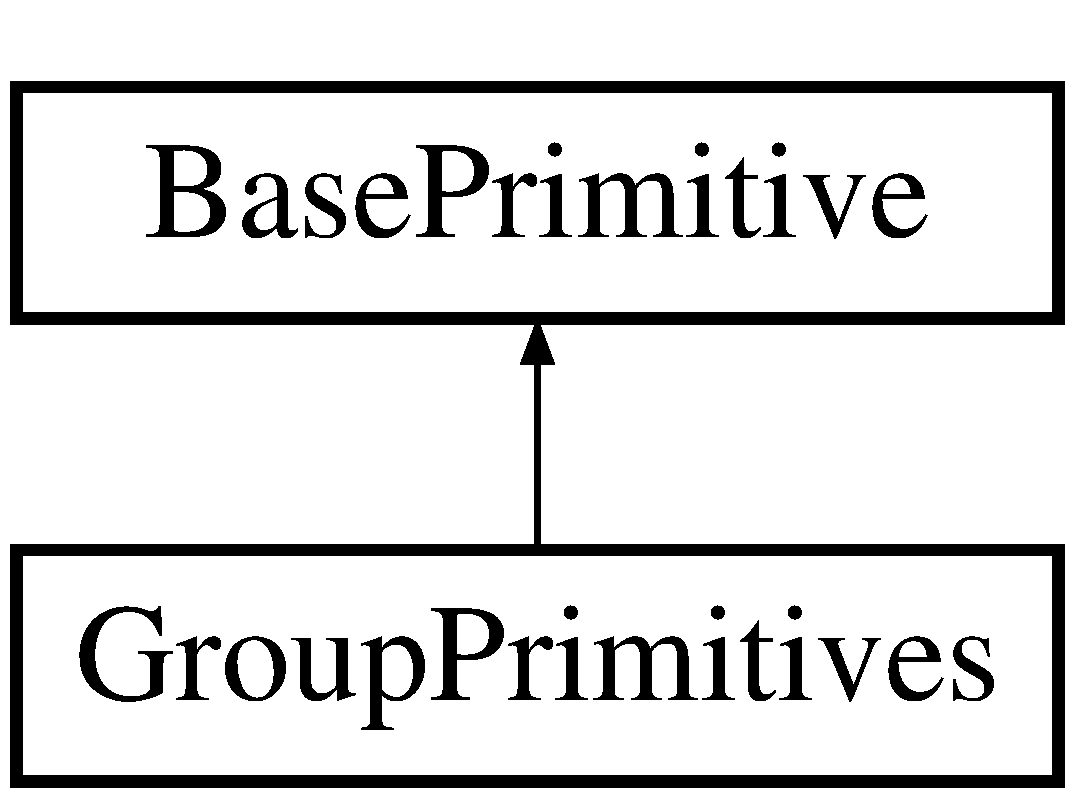
\includegraphics[height=2.000000cm]{class_base_primitive}
\end{center}
\end{figure}
\subsection*{Public Member Functions}
\begin{DoxyCompactItemize}
\item 
\mbox{\Hypertarget{class_base_primitive_a06a4cf2f143fc0eb478d3ab97b53c536}\label{class_base_primitive_a06a4cf2f143fc0eb478d3ab97b53c536}} 
\mbox{\hyperlink{class_base_primitive_a06a4cf2f143fc0eb478d3ab97b53c536}{Base\+Primitive}} ()
\begin{DoxyCompactList}\small\item\em Constructor. \end{DoxyCompactList}\item 
virtual bool \mbox{\hyperlink{class_base_primitive_a608aa970836909d21c0413d894612eca}{intersect}} (\mbox{\hyperlink{class_ray}{Ray}} \&ray, bool cull\+Back)=0
\item 
virtual bool \mbox{\hyperlink{class_base_primitive_a1f9cb5f2c71f2e1f985513a154f22712}{intersect}} (\mbox{\hyperlink{class_ray}{Ray}} \&ray, \mbox{\hyperlink{class_intersection}{Intersection}} \&intersection, bool cull\+Back)=0
\end{DoxyCompactItemize}


\subsection{Member Function Documentation}
\mbox{\Hypertarget{class_base_primitive_a608aa970836909d21c0413d894612eca}\label{class_base_primitive_a608aa970836909d21c0413d894612eca}} 
\index{Base\+Primitive@{Base\+Primitive}!intersect@{intersect}}
\index{intersect@{intersect}!Base\+Primitive@{Base\+Primitive}}
\subsubsection{\texorpdfstring{intersect()}{intersect()}\hspace{0.1cm}{\footnotesize\ttfamily [1/2]}}
{\footnotesize\ttfamily virtual bool Base\+Primitive\+::intersect (\begin{DoxyParamCaption}\item[{\mbox{\hyperlink{class_ray}{Ray}} \&}]{ray,  }\item[{bool}]{cull\+Back }\end{DoxyParamCaption})\hspace{0.3cm}{\ttfamily [pure virtual]}}

Test intersection between ray and this primitive 
\begin{DoxyParams}{Parameters}
{\em ray} & \\
\hline
{\em cull} & back face culling \\
\hline
\end{DoxyParams}
\begin{DoxyReturn}{Returns}
true for sucessfull intersection 
\end{DoxyReturn}


Implemented in \mbox{\hyperlink{class_group_primitives_a17bca38224e782eb6660774b34947397}{Group\+Primitives}}.

\mbox{\Hypertarget{class_base_primitive_a1f9cb5f2c71f2e1f985513a154f22712}\label{class_base_primitive_a1f9cb5f2c71f2e1f985513a154f22712}} 
\index{Base\+Primitive@{Base\+Primitive}!intersect@{intersect}}
\index{intersect@{intersect}!Base\+Primitive@{Base\+Primitive}}
\subsubsection{\texorpdfstring{intersect()}{intersect()}\hspace{0.1cm}{\footnotesize\ttfamily [2/2]}}
{\footnotesize\ttfamily virtual bool Base\+Primitive\+::intersect (\begin{DoxyParamCaption}\item[{\mbox{\hyperlink{class_ray}{Ray}} \&}]{ray,  }\item[{\mbox{\hyperlink{class_intersection}{Intersection}} \&}]{intersection,  }\item[{bool}]{cull\+Back }\end{DoxyParamCaption})\hspace{0.3cm}{\ttfamily [pure virtual]}}

Test intersection between ray and this primitive 
\begin{DoxyParams}[1]{Parameters}
 & {\em ray} & \\
\hline
\mbox{\tt in,out}  & {\em intersection} & will contain result of intersection \\
\hline
 & {\em cull} & back face culling \\
\hline
\end{DoxyParams}
\begin{DoxyReturn}{Returns}
true for sucessfull intersection 
\end{DoxyReturn}


Implemented in \mbox{\hyperlink{class_group_primitives_ac958af04e2e275f28cb74751ad87575a}{Group\+Primitives}}.



The documentation for this class was generated from the following file\+:\begin{DoxyCompactItemize}
\item 
\mbox{\hyperlink{base__primitive_8h}{base\+\_\+primitive.\+h}}\end{DoxyCompactItemize}

\hypertarget{class_camera}{}\section{Camera Class Reference}
\label{class_camera}\index{Camera@{Camera}}


{\ttfamily \#include $<$camera.\+h$>$}

\subsection*{Public Member Functions}
\begin{DoxyCompactItemize}
\item 
\mbox{\hyperlink{class_camera_aafce2ffd325ea7d8eb45076ba139ae17}{Camera}} (float fovy, float aspect, float near, float far)
\item 
void \mbox{\hyperlink{class_camera_afa27020f8305c918d9015bdebdb7437c}{look\+At}} (const \mbox{\hyperlink{struct_vector}{Vector}} \&campos, const \mbox{\hyperlink{struct_vector}{Vector}} \&lookat, const \mbox{\hyperlink{struct_vector}{Vector}} \&desiredup)
\item 
\mbox{\hyperlink{class_ray}{Ray}} \mbox{\hyperlink{class_camera_a154c1d086e33486104f1241692a5781c}{Generate\+Ray}} (\mbox{\hyperlink{struct_vector}{Vector}} \&sample)
\end{DoxyCompactItemize}
\subsection*{Public Attributes}
\begin{DoxyCompactItemize}
\item 
\mbox{\Hypertarget{class_camera_a181aff3db1ae87a837ddc3a97e5b0f43}\label{class_camera_a181aff3db1ae87a837ddc3a97e5b0f43}} 
float {\bfseries aspect}
\item 
\mbox{\Hypertarget{class_camera_aff7393c9cfbccd7e369091f00008da93}\label{class_camera_aff7393c9cfbccd7e369091f00008da93}} 
float {\bfseries fov}
\item 
\mbox{\Hypertarget{class_camera_ad96efd3e1e4ec33dddb1d25f05d02ff2}\label{class_camera_ad96efd3e1e4ec33dddb1d25f05d02ff2}} 
float {\bfseries near}
\item 
\mbox{\Hypertarget{class_camera_a9f30b77edf6485e001a98d21ff5f17fe}\label{class_camera_a9f30b77edf6485e001a98d21ff5f17fe}} 
float {\bfseries far}
\item 
\mbox{\Hypertarget{class_camera_a7f6914ba4267e8829c8199f1a61e24d7}\label{class_camera_a7f6914ba4267e8829c8199f1a61e24d7}} 
float {\bfseries tanfov}
\item 
\mbox{\Hypertarget{class_camera_a4d4c7ba071d86c1e890be73923dac2d1}\label{class_camera_a4d4c7ba071d86c1e890be73923dac2d1}} 
\mbox{\hyperlink{struct_vector}{Vector}} {\bfseries pos}
\item 
\mbox{\Hypertarget{class_camera_af628dbd4dc8e60240db45825ecea0d81}\label{class_camera_af628dbd4dc8e60240db45825ecea0d81}} 
\mbox{\hyperlink{struct_vector}{Vector}} {\bfseries dir}
\item 
\mbox{\Hypertarget{class_camera_ae6748e11785b98e30118c5ed16dc461b}\label{class_camera_ae6748e11785b98e30118c5ed16dc461b}} 
mat4 {\bfseries world\+To\+UV}
\item 
\mbox{\Hypertarget{class_camera_a1921c5ccd90c4e1b27db25947c2b083e}\label{class_camera_a1921c5ccd90c4e1b27db25947c2b083e}} 
mat4 {\bfseries uv\+To\+World}
\item 
\mbox{\Hypertarget{class_camera_a30128269cb562b51010db9ffb39edbc4}\label{class_camera_a30128269cb562b51010db9ffb39edbc4}} 
\mbox{\hyperlink{class_transform}{Transform}} {\bfseries projection}
\item 
\mbox{\Hypertarget{class_camera_ad7f51fc63f1e028a87fea720943b481c}\label{class_camera_ad7f51fc63f1e028a87fea720943b481c}} 
\mbox{\hyperlink{class_transform}{Transform}} {\bfseries world\+To\+Camera}
\item 
\mbox{\Hypertarget{class_camera_a1a9bab596e1d324368630d7606d186f5}\label{class_camera_a1a9bab596e1d324368630d7606d186f5}} 
\mbox{\hyperlink{class_transform}{Transform}} {\bfseries camera\+To\+World}
\end{DoxyCompactItemize}


\subsection{Detailed Description}
Simple camera for ray tracer 

\subsection{Constructor \& Destructor Documentation}
\mbox{\Hypertarget{class_camera_aafce2ffd325ea7d8eb45076ba139ae17}\label{class_camera_aafce2ffd325ea7d8eb45076ba139ae17}} 
\index{Camera@{Camera}!Camera@{Camera}}
\index{Camera@{Camera}!Camera@{Camera}}
\subsubsection{\texorpdfstring{Camera()}{Camera()}}
{\footnotesize\ttfamily Camera\+::\+Camera (\begin{DoxyParamCaption}\item[{float}]{fovy,  }\item[{float}]{aspect,  }\item[{float}]{near,  }\item[{float}]{far }\end{DoxyParamCaption})\hspace{0.3cm}{\ttfamily [inline]}}

Construct new camera 
\begin{DoxyParams}{Parameters}
{\em fovy} & vertical field of view \\
\hline
{\em aspect} & aspect ratio \\
\hline
{\em near} & distance to near plane \\
\hline
{\em far} & distance to far plane \\
\hline
\end{DoxyParams}


\subsection{Member Function Documentation}
\mbox{\Hypertarget{class_camera_a154c1d086e33486104f1241692a5781c}\label{class_camera_a154c1d086e33486104f1241692a5781c}} 
\index{Camera@{Camera}!Generate\+Ray@{Generate\+Ray}}
\index{Generate\+Ray@{Generate\+Ray}!Camera@{Camera}}
\subsubsection{\texorpdfstring{Generate\+Ray()}{GenerateRay()}}
{\footnotesize\ttfamily \mbox{\hyperlink{class_ray}{Ray}} Camera\+::\+Generate\+Ray (\begin{DoxyParamCaption}\item[{\mbox{\hyperlink{struct_vector}{Vector}} \&}]{sample }\end{DoxyParamCaption})\hspace{0.3cm}{\ttfamily [inline]}}

Generate camera ray 
\begin{DoxyParams}{Parameters}
{\em sample} & coordinate of sample \\
\hline
\end{DoxyParams}
\begin{DoxyReturn}{Returns}
new ray for this sample point 
\end{DoxyReturn}
\mbox{\Hypertarget{class_camera_afa27020f8305c918d9015bdebdb7437c}\label{class_camera_afa27020f8305c918d9015bdebdb7437c}} 
\index{Camera@{Camera}!look\+At@{look\+At}}
\index{look\+At@{look\+At}!Camera@{Camera}}
\subsubsection{\texorpdfstring{look\+At()}{lookAt()}}
{\footnotesize\ttfamily void Camera\+::look\+At (\begin{DoxyParamCaption}\item[{const \mbox{\hyperlink{struct_vector}{Vector}} \&}]{campos,  }\item[{const \mbox{\hyperlink{struct_vector}{Vector}} \&}]{lookat,  }\item[{const \mbox{\hyperlink{struct_vector}{Vector}} \&}]{desiredup }\end{DoxyParamCaption})\hspace{0.3cm}{\ttfamily [inline]}}

Set camera transform to position and \textquotesingle{}look at\textquotesingle{} orientation 
\begin{DoxyParams}{Parameters}
{\em campos} & camera position \\
\hline
{\em lookat} & look at point \\
\hline
{\em desiredup} & vector up \\
\hline
\end{DoxyParams}


The documentation for this class was generated from the following file\+:\begin{DoxyCompactItemize}
\item 
\mbox{\hyperlink{camera_8h}{camera.\+h}}\end{DoxyCompactItemize}

\hypertarget{class_color}{}\section{Color Class Reference}
\label{class_color}\index{Color@{Color}}


{\ttfamily \#include $<$color.\+h$>$}

\subsection*{Public Member Functions}
\begin{DoxyCompactItemize}
\item 
\mbox{\Hypertarget{class_color_a9a742cbe9f9f4037f5d9f4e81a9b2428}\label{class_color_a9a742cbe9f9f4037f5d9f4e81a9b2428}} 
\mbox{\hyperlink{class_color_a9a742cbe9f9f4037f5d9f4e81a9b2428}{Color}} ()
\begin{DoxyCompactList}\small\item\em Construct default, black color. \end{DoxyCompactList}\item 
\mbox{\Hypertarget{class_color_a24e9f1b022bec1e1ace02ed2956335b5}\label{class_color_a24e9f1b022bec1e1ace02ed2956335b5}} 
\mbox{\hyperlink{class_color_a24e9f1b022bec1e1ace02ed2956335b5}{Color}} (float ri, float gi, float bi)
\begin{DoxyCompactList}\small\item\em Construct color with given componen\textquotesingle{}s values. \end{DoxyCompactList}\item 
\mbox{\Hypertarget{class_color_af41b1bebc47df170ba61176c739be64b}\label{class_color_af41b1bebc47df170ba61176c739be64b}} 
\mbox{\hyperlink{class_color_af41b1bebc47df170ba61176c739be64b}{Color}} (const \mbox{\hyperlink{struct_vector}{Vector}} \&v)
\begin{DoxyCompactList}\small\item\em Construct color from the vector value. \end{DoxyCompactList}\item 
void \mbox{\hyperlink{class_color_abe5a97a40715b5474aca1576dcf0f3bd}{Set}} (float ri, float gi, float bi)
\item 
\mbox{\hyperlink{class_color}{Color}} \mbox{\hyperlink{class_color_ad752bd0184c61b0afd86fe11f1472633}{operator$\ast$}} (float c) const
\item 
\mbox{\hyperlink{class_color}{Color}} \mbox{\hyperlink{class_color_a7937d45e05eacfa19174171743f612c6}{operator+}} (float c) const
\item 
\mbox{\hyperlink{class_color}{Color}} \mbox{\hyperlink{class_color_acf63f968ca0decdd119164e206807693}{operator-\/}} (float c) const
\item 
\mbox{\Hypertarget{class_color_ae4ca68c5d5680cc03060be1141d4abb6}\label{class_color_ae4ca68c5d5680cc03060be1141d4abb6}} 
\mbox{\hyperlink{class_color}{Color}} \mbox{\hyperlink{class_color_ae4ca68c5d5680cc03060be1141d4abb6}{operator$\ast$}} (const \mbox{\hyperlink{class_color}{Color}} \&c) const
\begin{DoxyCompactList}\small\item\em Multiply two colors. \end{DoxyCompactList}\item 
\mbox{\Hypertarget{class_color_a54ce5844ba0c0bed7b155f630b9c8e23}\label{class_color_a54ce5844ba0c0bed7b155f630b9c8e23}} 
\mbox{\hyperlink{class_color}{Color}} \mbox{\hyperlink{class_color_a54ce5844ba0c0bed7b155f630b9c8e23}{operator+}} (const \mbox{\hyperlink{class_color}{Color}} \&c) const
\begin{DoxyCompactList}\small\item\em Summ of two colors. \end{DoxyCompactList}\item 
\mbox{\Hypertarget{class_color_aad136d208cedd7d68f3783ecc6ccdce8}\label{class_color_aad136d208cedd7d68f3783ecc6ccdce8}} 
\mbox{\hyperlink{class_color}{Color}} \mbox{\hyperlink{class_color_aad136d208cedd7d68f3783ecc6ccdce8}{operator-\/}} (const \mbox{\hyperlink{class_color}{Color}} \&c) const
\begin{DoxyCompactList}\small\item\em Difference of two colors. \end{DoxyCompactList}\item 
\mbox{\Hypertarget{class_color_aa73c992c7e31bb11aa1f810b19d5fe4c}\label{class_color_aa73c992c7e31bb11aa1f810b19d5fe4c}} 
\mbox{\hyperlink{class_color}{Color}} \& \mbox{\hyperlink{class_color_aa73c992c7e31bb11aa1f810b19d5fe4c}{operator$\ast$=}} (const \mbox{\hyperlink{class_color}{Color}} \&c)
\begin{DoxyCompactList}\small\item\em Multiply two colors. \end{DoxyCompactList}\item 
\mbox{\Hypertarget{class_color_a88c2bdadb4a02ae8cfeb7f1c6952b196}\label{class_color_a88c2bdadb4a02ae8cfeb7f1c6952b196}} 
\mbox{\hyperlink{class_color}{Color}} \& \mbox{\hyperlink{class_color_a88c2bdadb4a02ae8cfeb7f1c6952b196}{operator+=}} (const \mbox{\hyperlink{class_color}{Color}} \&c)
\begin{DoxyCompactList}\small\item\em Summ of two colors. \end{DoxyCompactList}\item 
\mbox{\Hypertarget{class_color_a75c5f84de36f941c9c6471e6423ad6da}\label{class_color_a75c5f84de36f941c9c6471e6423ad6da}} 
\mbox{\hyperlink{class_color}{Color}} \& \mbox{\hyperlink{class_color_a75c5f84de36f941c9c6471e6423ad6da}{operator-\/=}} (const \mbox{\hyperlink{class_color}{Color}} \&c)
\begin{DoxyCompactList}\small\item\em Difference of two colors. \end{DoxyCompactList}\item 
\mbox{\Hypertarget{class_color_ae1af5e1afd54bde2e229586410d2adc4}\label{class_color_ae1af5e1afd54bde2e229586410d2adc4}} 
\mbox{\hyperlink{class_color}{Color}} \& \mbox{\hyperlink{class_color_ae1af5e1afd54bde2e229586410d2adc4}{operator$\ast$=}} (float c)
\begin{DoxyCompactList}\small\item\em Multiply color by scalar value. \end{DoxyCompactList}\item 
bool \mbox{\hyperlink{class_color_a28a6f5a2125403d7d8ad35f793db21ca}{is\+Zero}} ()
\end{DoxyCompactItemize}
\subsection*{Public Attributes}
\textbf{ }\par
\begin{DoxyCompactItemize}
\item 
float \mbox{\hyperlink{class_color_a3958a556b47d2de3dd45c75aac833c20}{r}}
\item 
float \mbox{\hyperlink{class_color_a5defbb21620e480e556181772d665f34}{g}}
\item 
float \mbox{\hyperlink{class_color_a33e482be18d6ea31d2b403bee13683b7}{b}}
\end{DoxyCompactItemize}



\subsection{Detailed Description}
The \mbox{\hyperlink{class_color}{Color}} class. Contains r,g,b components only. 

\subsection{Member Function Documentation}
\mbox{\Hypertarget{class_color_a28a6f5a2125403d7d8ad35f793db21ca}\label{class_color_a28a6f5a2125403d7d8ad35f793db21ca}} 
\index{Color@{Color}!is\+Zero@{is\+Zero}}
\index{is\+Zero@{is\+Zero}!Color@{Color}}
\subsubsection{\texorpdfstring{is\+Zero()}{isZero()}}
{\footnotesize\ttfamily bool Color\+::is\+Zero (\begin{DoxyParamCaption}{ }\end{DoxyParamCaption})\hspace{0.3cm}{\ttfamily [inline]}}

\begin{DoxyReturn}{Returns}
true if this color fully black 
\end{DoxyReturn}
\mbox{\Hypertarget{class_color_ad752bd0184c61b0afd86fe11f1472633}\label{class_color_ad752bd0184c61b0afd86fe11f1472633}} 
\index{Color@{Color}!operator$\ast$@{operator$\ast$}}
\index{operator$\ast$@{operator$\ast$}!Color@{Color}}
\subsubsection{\texorpdfstring{operator$\ast$()}{operator*()}}
{\footnotesize\ttfamily \mbox{\hyperlink{class_color}{Color}} Color\+::operator$\ast$ (\begin{DoxyParamCaption}\item[{float}]{c }\end{DoxyParamCaption}) const\hspace{0.3cm}{\ttfamily [inline]}}

Magnitude the color 
\begin{DoxyParams}{Parameters}
{\em c} & scalar value \\
\hline
\end{DoxyParams}
\mbox{\Hypertarget{class_color_a7937d45e05eacfa19174171743f612c6}\label{class_color_a7937d45e05eacfa19174171743f612c6}} 
\index{Color@{Color}!operator+@{operator+}}
\index{operator+@{operator+}!Color@{Color}}
\subsubsection{\texorpdfstring{operator+()}{operator+()}}
{\footnotesize\ttfamily \mbox{\hyperlink{class_color}{Color}} Color\+::operator+ (\begin{DoxyParamCaption}\item[{float}]{c }\end{DoxyParamCaption}) const\hspace{0.3cm}{\ttfamily [inline]}}

Increase brigness of this color (aka ambient light) 
\begin{DoxyParams}{Parameters}
{\em c} & scalar value \\
\hline
\end{DoxyParams}
\mbox{\Hypertarget{class_color_acf63f968ca0decdd119164e206807693}\label{class_color_acf63f968ca0decdd119164e206807693}} 
\index{Color@{Color}!operator-\/@{operator-\/}}
\index{operator-\/@{operator-\/}!Color@{Color}}
\subsubsection{\texorpdfstring{operator-\/()}{operator-()}}
{\footnotesize\ttfamily \mbox{\hyperlink{class_color}{Color}} Color\+::operator-\/ (\begin{DoxyParamCaption}\item[{float}]{c }\end{DoxyParamCaption}) const\hspace{0.3cm}{\ttfamily [inline]}}

Decrease brigness of this color (aka ambient light) 
\begin{DoxyParams}{Parameters}
{\em c} & scalar value \\
\hline
\end{DoxyParams}
\mbox{\Hypertarget{class_color_abe5a97a40715b5474aca1576dcf0f3bd}\label{class_color_abe5a97a40715b5474aca1576dcf0f3bd}} 
\index{Color@{Color}!Set@{Set}}
\index{Set@{Set}!Color@{Color}}
\subsubsection{\texorpdfstring{Set()}{Set()}}
{\footnotesize\ttfamily void Color\+::\+Set (\begin{DoxyParamCaption}\item[{float}]{ri,  }\item[{float}]{gi,  }\item[{float}]{bi }\end{DoxyParamCaption})\hspace{0.3cm}{\ttfamily [inline]}}

Set color 
\begin{DoxyParams}{Parameters}
{\em ri} & component \\
\hline
{\em gi} & component \\
\hline
{\em bi} & component \\
\hline
\end{DoxyParams}


\subsection{Member Data Documentation}
\mbox{\Hypertarget{class_color_a33e482be18d6ea31d2b403bee13683b7}\label{class_color_a33e482be18d6ea31d2b403bee13683b7}} 
\index{Color@{Color}!b@{b}}
\index{b@{b}!Color@{Color}}
\subsubsection{\texorpdfstring{b}{b}}
{\footnotesize\ttfamily float Color\+::b}

The color component \mbox{\Hypertarget{class_color_a5defbb21620e480e556181772d665f34}\label{class_color_a5defbb21620e480e556181772d665f34}} 
\index{Color@{Color}!g@{g}}
\index{g@{g}!Color@{Color}}
\subsubsection{\texorpdfstring{g}{g}}
{\footnotesize\ttfamily float Color\+::g}

The color component \mbox{\Hypertarget{class_color_a3958a556b47d2de3dd45c75aac833c20}\label{class_color_a3958a556b47d2de3dd45c75aac833c20}} 
\index{Color@{Color}!r@{r}}
\index{r@{r}!Color@{Color}}
\subsubsection{\texorpdfstring{r}{r}}
{\footnotesize\ttfamily float Color\+::r}

The color component 

The documentation for this class was generated from the following file\+:\begin{DoxyCompactItemize}
\item 
\mbox{\hyperlink{color_8h}{color.\+h}}\end{DoxyCompactItemize}

\hypertarget{class_group_primitives}{}\section{Group\+Primitives Class Reference}
\label{class_group_primitives}\index{Group\+Primitives@{Group\+Primitives}}


{\ttfamily \#include $<$group\+\_\+primitives.\+h$>$}

Inheritance diagram for Group\+Primitives\+:\begin{figure}[H]
\begin{center}
\leavevmode
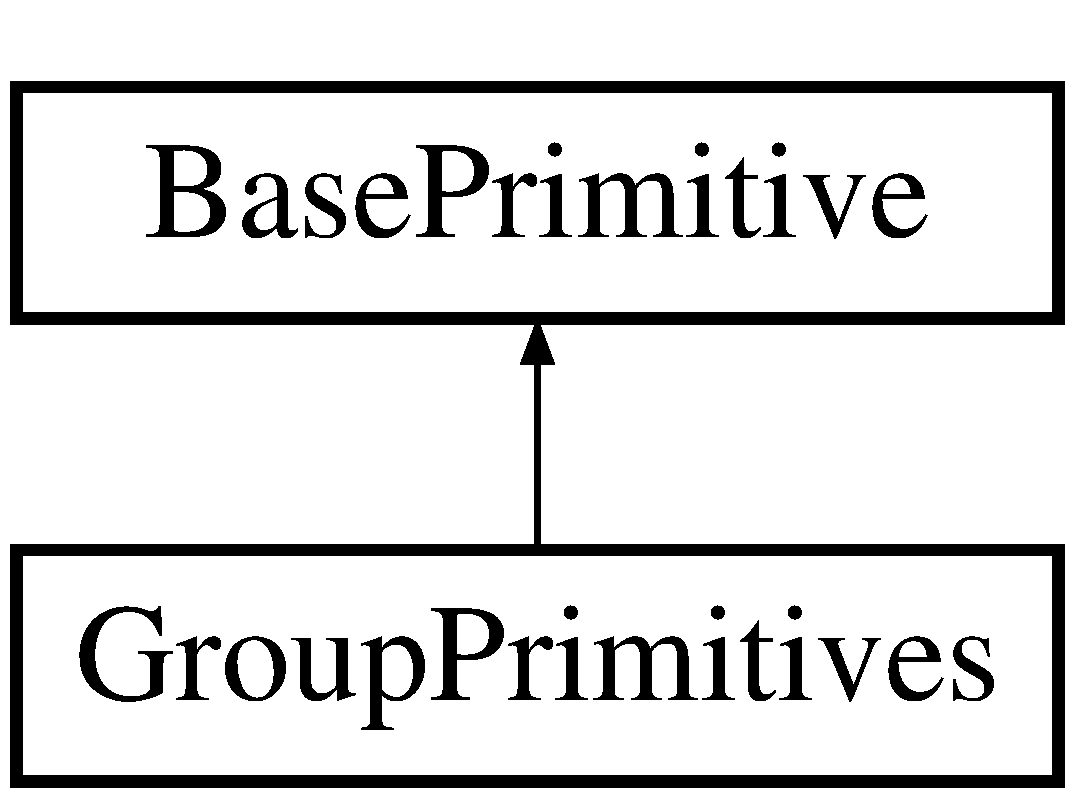
\includegraphics[height=2.000000cm]{class_group_primitives}
\end{center}
\end{figure}
\subsection*{Public Member Functions}
\begin{DoxyCompactItemize}
\item 
\mbox{\hyperlink{class_group_primitives_ad09cb3eb5220543a5edf1f85a38e7244}{Group\+Primitives}} (std\+::vector$<$ \mbox{\hyperlink{class_primitive}{Primitive}} $\ast$$>$ primitives\+List)
\item 
\mbox{\hyperlink{class_group_primitives_a821c2b3b8a794ad486e518e313403e8f}{Group\+Primitives}} (std\+::vector$<$ \mbox{\hyperlink{class_primitive}{Primitive}} $\ast$$>$ primitives\+List, const \mbox{\hyperlink{struct_vector}{Vector}} \&light\+Dir)
\item 
void \mbox{\hyperlink{class_group_primitives_ace5b8c68e4a9f26416ccc4ab9ced8525}{set\+Primitives}} (std\+::vector$<$ \mbox{\hyperlink{class_primitive}{Primitive}} $\ast$$>$ primitives\+List, const \mbox{\hyperlink{struct_vector}{Vector}} \&light\+Dir)
\item 
virtual bool \mbox{\hyperlink{class_group_primitives_a17bca38224e782eb6660774b34947397}{intersect}} (\mbox{\hyperlink{class_ray}{Ray}} \&ray, bool cull\+Back)
\item 
virtual bool \mbox{\hyperlink{class_group_primitives_ac958af04e2e275f28cb74751ad87575a}{intersect}} (\mbox{\hyperlink{class_ray}{Ray}} \&ray, \mbox{\hyperlink{class_intersection}{Intersection}} \&intersection, bool cull\+Back)
\end{DoxyCompactItemize}
\subsection*{Public Attributes}
\begin{DoxyCompactItemize}
\item 
\mbox{\Hypertarget{class_group_primitives_a694241c5449d75ea29669e4cc7d93d32}\label{class_group_primitives_a694241c5449d75ea29669e4cc7d93d32}} 
std\+::vector$<$ \mbox{\hyperlink{class_primitive}{Primitive}} $\ast$ $>$ \mbox{\hyperlink{class_group_primitives_a694241c5449d75ea29669e4cc7d93d32}{primitives}}
\begin{DoxyCompactList}\small\item\em The collection of primitive. \end{DoxyCompactList}\end{DoxyCompactItemize}


\subsection{Detailed Description}
\mbox{\hyperlink{class_group_primitives}{Group\+Primitives}}

Methods\+:

\mbox{\hyperlink{class_group_primitives}{Group\+Primitives(vector$<$\+Primitive$\ast$$>$ list)}};

bool intersect(\+Ray\& ray, float$\ast$ thit, Intersection$\ast$ in)

bool intersect\+P(\+Ray\& ray)

void get\+B\+R\+D\+F(\+Local\+Geo\& local, B\+R\+D\+F$\ast$ brdf) \{ exit(1); // This should never get called, because in-\/$>$primitive will // never be an aggregate primitive \}

Notes\+:

Constructor store the S\+TL vector of pointers to primitives. Intersect just loops through all the primitives in the list and call the intersect routine. Compare thit and return that of the nearest one (because we want the first hit).

Also, the in-\/$>$primitive should be set to the pointer to that primitive. When you implement acceleration structure, it will replace this class. 

\subsection{Constructor \& Destructor Documentation}
\mbox{\Hypertarget{class_group_primitives_ad09cb3eb5220543a5edf1f85a38e7244}\label{class_group_primitives_ad09cb3eb5220543a5edf1f85a38e7244}} 
\index{Group\+Primitives@{Group\+Primitives}!Group\+Primitives@{Group\+Primitives}}
\index{Group\+Primitives@{Group\+Primitives}!Group\+Primitives@{Group\+Primitives}}
\subsubsection{\texorpdfstring{Group\+Primitives()}{GroupPrimitives()}\hspace{0.1cm}{\footnotesize\ttfamily [1/2]}}
{\footnotesize\ttfamily Group\+Primitives\+::\+Group\+Primitives (\begin{DoxyParamCaption}\item[{std\+::vector$<$ \mbox{\hyperlink{class_primitive}{Primitive}} $\ast$$>$}]{primitives\+List }\end{DoxyParamCaption})\hspace{0.3cm}{\ttfamily [inline]}}

Constructor with collection of primitives 
\begin{DoxyParams}{Parameters}
{\em primitives\+List} & the collection of primitives \\
\hline
\end{DoxyParams}
\mbox{\Hypertarget{class_group_primitives_a821c2b3b8a794ad486e518e313403e8f}\label{class_group_primitives_a821c2b3b8a794ad486e518e313403e8f}} 
\index{Group\+Primitives@{Group\+Primitives}!Group\+Primitives@{Group\+Primitives}}
\index{Group\+Primitives@{Group\+Primitives}!Group\+Primitives@{Group\+Primitives}}
\subsubsection{\texorpdfstring{Group\+Primitives()}{GroupPrimitives()}\hspace{0.1cm}{\footnotesize\ttfamily [2/2]}}
{\footnotesize\ttfamily Group\+Primitives\+::\+Group\+Primitives (\begin{DoxyParamCaption}\item[{std\+::vector$<$ \mbox{\hyperlink{class_primitive}{Primitive}} $\ast$$>$}]{primitives\+List,  }\item[{const \mbox{\hyperlink{struct_vector}{Vector}} \&}]{light\+Dir }\end{DoxyParamCaption})\hspace{0.3cm}{\ttfamily [inline]}}

Constructor this with collection of primitives. The method will use only faces oriented to the given dirrection 
\begin{DoxyParams}{Parameters}
{\em primitives\+List} & the collection of primitives \\
\hline
{\em light\+Dir} & direction of light \\
\hline
\end{DoxyParams}


\subsection{Member Function Documentation}
\mbox{\Hypertarget{class_group_primitives_a17bca38224e782eb6660774b34947397}\label{class_group_primitives_a17bca38224e782eb6660774b34947397}} 
\index{Group\+Primitives@{Group\+Primitives}!intersect@{intersect}}
\index{intersect@{intersect}!Group\+Primitives@{Group\+Primitives}}
\subsubsection{\texorpdfstring{intersect()}{intersect()}\hspace{0.1cm}{\footnotesize\ttfamily [1/2]}}
{\footnotesize\ttfamily virtual bool Group\+Primitives\+::intersect (\begin{DoxyParamCaption}\item[{\mbox{\hyperlink{class_ray}{Ray}} \&}]{ray,  }\item[{bool}]{cull\+Back }\end{DoxyParamCaption})\hspace{0.3cm}{\ttfamily [inline]}, {\ttfamily [virtual]}}

Test intersection between ray and this primitive 
\begin{DoxyParams}{Parameters}
{\em ray} & \\
\hline
{\em cull} & back face culling \\
\hline
\end{DoxyParams}
\begin{DoxyReturn}{Returns}
true for sucessfull intersection 
\end{DoxyReturn}


Implements \mbox{\hyperlink{class_base_primitive_a608aa970836909d21c0413d894612eca}{Base\+Primitive}}.

\mbox{\Hypertarget{class_group_primitives_ac958af04e2e275f28cb74751ad87575a}\label{class_group_primitives_ac958af04e2e275f28cb74751ad87575a}} 
\index{Group\+Primitives@{Group\+Primitives}!intersect@{intersect}}
\index{intersect@{intersect}!Group\+Primitives@{Group\+Primitives}}
\subsubsection{\texorpdfstring{intersect()}{intersect()}\hspace{0.1cm}{\footnotesize\ttfamily [2/2]}}
{\footnotesize\ttfamily virtual bool Group\+Primitives\+::intersect (\begin{DoxyParamCaption}\item[{\mbox{\hyperlink{class_ray}{Ray}} \&}]{ray,  }\item[{\mbox{\hyperlink{class_intersection}{Intersection}} \&}]{intersection,  }\item[{bool}]{cull\+Back }\end{DoxyParamCaption})\hspace{0.3cm}{\ttfamily [inline]}, {\ttfamily [virtual]}}

Test intersection between ray and this primitive 
\begin{DoxyParams}[1]{Parameters}
 & {\em ray} & \\
\hline
\mbox{\tt in,out}  & {\em intersection} & will contain result of intersection \\
\hline
 & {\em cull} & back face culling \\
\hline
\end{DoxyParams}
\begin{DoxyReturn}{Returns}
true for sucessfull intersection 
\end{DoxyReturn}


Implements \mbox{\hyperlink{class_base_primitive_a1f9cb5f2c71f2e1f985513a154f22712}{Base\+Primitive}}.

\mbox{\Hypertarget{class_group_primitives_ace5b8c68e4a9f26416ccc4ab9ced8525}\label{class_group_primitives_ace5b8c68e4a9f26416ccc4ab9ced8525}} 
\index{Group\+Primitives@{Group\+Primitives}!set\+Primitives@{set\+Primitives}}
\index{set\+Primitives@{set\+Primitives}!Group\+Primitives@{Group\+Primitives}}
\subsubsection{\texorpdfstring{set\+Primitives()}{setPrimitives()}}
{\footnotesize\ttfamily void Group\+Primitives\+::set\+Primitives (\begin{DoxyParamCaption}\item[{std\+::vector$<$ \mbox{\hyperlink{class_primitive}{Primitive}} $\ast$$>$}]{primitives\+List,  }\item[{const \mbox{\hyperlink{struct_vector}{Vector}} \&}]{light\+Dir }\end{DoxyParamCaption})\hspace{0.3cm}{\ttfamily [inline]}}

Set primitives. The method will use only faces oriented to the given dirrection 
\begin{DoxyParams}{Parameters}
{\em primitives\+List} & the collection of primitives \\
\hline
{\em light\+Dir} & direction of light \\
\hline
\end{DoxyParams}


The documentation for this class was generated from the following file\+:\begin{DoxyCompactItemize}
\item 
\mbox{\hyperlink{group__primitives_8h}{group\+\_\+primitives.\+h}}\end{DoxyCompactItemize}

\hypertarget{class_intersection}{}\section{Intersection Class Reference}
\label{class_intersection}\index{Intersection@{Intersection}}


{\ttfamily \#include $<$intersection.\+h$>$}

\subsection*{Public Member Functions}
\begin{DoxyCompactItemize}
\item 
\mbox{\Hypertarget{class_intersection_a67497e3efe2793b23909052eeb82c4f3}\label{class_intersection_a67497e3efe2793b23909052eeb82c4f3}} 
\mbox{\hyperlink{class_intersection_a67497e3efe2793b23909052eeb82c4f3}{Intersection}} ()
\begin{DoxyCompactList}\small\item\em Construct intersection. \end{DoxyCompactList}\end{DoxyCompactItemize}
\subsection*{Public Attributes}
\begin{DoxyCompactItemize}
\item 
\mbox{\Hypertarget{class_intersection_a80de47d40c5d3a8a7079cc13412be5e7}\label{class_intersection_a80de47d40c5d3a8a7079cc13412be5e7}} 
\mbox{\hyperlink{class_primitive}{Primitive}} $\ast$ \mbox{\hyperlink{class_intersection_a80de47d40c5d3a8a7079cc13412be5e7}{primitive}}
\begin{DoxyCompactList}\small\item\em Pinter to primitive. \end{DoxyCompactList}\item 
\mbox{\Hypertarget{class_intersection_a2f432340bee6925251ec4e7895ac3a39}\label{class_intersection_a2f432340bee6925251ec4e7895ac3a39}} 
\mbox{\hyperlink{class_surface_point}{Surface\+Point}} \mbox{\hyperlink{class_intersection_a2f432340bee6925251ec4e7895ac3a39}{surface\+Point}}
\begin{DoxyCompactList}\small\item\em Collision point. \end{DoxyCompactList}\item 
\mbox{\Hypertarget{class_intersection_a65da854f067b6f08175a97d262a17f1e}\label{class_intersection_a65da854f067b6f08175a97d262a17f1e}} 
double \mbox{\hyperlink{class_intersection_a65da854f067b6f08175a97d262a17f1e}{distance}}
\begin{DoxyCompactList}\small\item\em Distance to intersection. \end{DoxyCompactList}\end{DoxyCompactItemize}


\subsection{Detailed Description}
\mbox{\hyperlink{class_intersection}{Intersection}}

Members\+: Collision\+Point local\+Geo Primitive$\ast$ primitive 

The documentation for this class was generated from the following file\+:\begin{DoxyCompactItemize}
\item 
\mbox{\hyperlink{intersection_8h}{intersection.\+h}}\end{DoxyCompactItemize}

\hypertarget{class_light}{}\section{Light Class Reference}
\label{class_light}\index{Light@{Light}}


{\ttfamily \#include $<$light.\+h$>$}

\subsection*{Public Member Functions}
\begin{DoxyCompactItemize}
\item 
\mbox{\hyperlink{class_light_a69ca971ea95f41b226e12e02094ba1f2}{Light}} (float x, float y, float z, float r, float g, float b, bool is\+\_\+point)
\item 
\mbox{\Hypertarget{class_light_acfc5fe7c64a270977b3a5a2e53a0fb9c}\label{class_light_acfc5fe7c64a270977b3a5a2e53a0fb9c}} 
\mbox{\hyperlink{class_ray}{Ray}} {\bfseries get\+Ray} (const \mbox{\hyperlink{class_surface_point}{Surface\+Point}} \&surf\+Point)
\item 
\mbox{\hyperlink{class_color}{Color}} \mbox{\hyperlink{class_light_a0fb5b95b28c59924030681c0d2646e87}{get\+Color}} (const \mbox{\hyperlink{class_ray}{Ray}} \&ray)
\end{DoxyCompactItemize}
\subsection*{Public Attributes}
\begin{DoxyCompactItemize}
\item 
\mbox{\Hypertarget{class_light_a88ff3e89ced966a6a882ac57483b500b}\label{class_light_a88ff3e89ced966a6a882ac57483b500b}} 
bool {\bfseries is\+Point}
\item 
\mbox{\Hypertarget{class_light_a48927a23d97db2c956d0b206fbe06be2}\label{class_light_a48927a23d97db2c956d0b206fbe06be2}} 
\mbox{\hyperlink{struct_vector}{Vector}} {\bfseries pos}
\item 
\mbox{\Hypertarget{class_light_ad7a168d26aed1bf7cca1a8d8e6f8ada4}\label{class_light_ad7a168d26aed1bf7cca1a8d8e6f8ada4}} 
\mbox{\hyperlink{class_color}{Color}} {\bfseries color}
\item 
float \mbox{\hyperlink{class_light_a27af00db907fd279ba3e342d6c5ec8c2}{attenuation\+Const}}
\item 
\mbox{\Hypertarget{class_light_a6fe2e610682fa03bdb3d5a3036c0ec4a}\label{class_light_a6fe2e610682fa03bdb3d5a3036c0ec4a}} 
float {\bfseries attenuation\+Linear}
\item 
\mbox{\Hypertarget{class_light_a1208ffdf5fd52614c5fd2b6ea787921c}\label{class_light_a1208ffdf5fd52614c5fd2b6ea787921c}} 
float {\bfseries attenuation\+Quadratic}
\end{DoxyCompactItemize}


\subsection{Detailed Description}
\mbox{\hyperlink{class_light}{Light}}

Methods\+:

void generate\+Light\+Ray(\+Local\+Geo\& local, Ray$\ast$ lray, Color$\ast$ lcolor);

Notes\+:

This is an abstract class that will generate a ray starting from the position stored in local to the position of the light source.

You might want to consider creating 2 derived classes for point light source and directional light source. For directional light, the origin of the ray is the same, and the ray points to the light direction, however, t\+\_\+max is infinity. 

\subsection{Constructor \& Destructor Documentation}
\mbox{\Hypertarget{class_light_a69ca971ea95f41b226e12e02094ba1f2}\label{class_light_a69ca971ea95f41b226e12e02094ba1f2}} 
\index{Light@{Light}!Light@{Light}}
\index{Light@{Light}!Light@{Light}}
\subsubsection{\texorpdfstring{Light()}{Light()}}
{\footnotesize\ttfamily Light\+::\+Light (\begin{DoxyParamCaption}\item[{float}]{x,  }\item[{float}]{y,  }\item[{float}]{z,  }\item[{float}]{r,  }\item[{float}]{g,  }\item[{float}]{b,  }\item[{bool}]{is\+\_\+point }\end{DoxyParamCaption})\hspace{0.3cm}{\ttfamily [inline]}}

Create light source 
\begin{DoxyParams}{Parameters}
{\em x} & position \\
\hline
{\em y} & position \\
\hline
{\em z} & position \\
\hline
{\em r} & color \\
\hline
{\em g} & color \\
\hline
{\em b} & color \\
\hline
{\em is\+\_\+point} & is point light? Other case directional \\
\hline
\end{DoxyParams}


\subsection{Member Function Documentation}
\mbox{\Hypertarget{class_light_a0fb5b95b28c59924030681c0d2646e87}\label{class_light_a0fb5b95b28c59924030681c0d2646e87}} 
\index{Light@{Light}!get\+Color@{get\+Color}}
\index{get\+Color@{get\+Color}!Light@{Light}}
\subsubsection{\texorpdfstring{get\+Color()}{getColor()}}
{\footnotesize\ttfamily \mbox{\hyperlink{class_color}{Color}} Light\+::get\+Color (\begin{DoxyParamCaption}\item[{const \mbox{\hyperlink{class_ray}{Ray}} \&}]{ray }\end{DoxyParamCaption})\hspace{0.3cm}{\ttfamily [inline]}}

get color of light for given ray 
\begin{DoxyParams}{Parameters}
{\em ray} & to the light \\
\hline
\end{DoxyParams}


\subsection{Member Data Documentation}
\mbox{\Hypertarget{class_light_a27af00db907fd279ba3e342d6c5ec8c2}\label{class_light_a27af00db907fd279ba3e342d6c5ec8c2}} 
\index{Light@{Light}!attenuation\+Const@{attenuation\+Const}}
\index{attenuation\+Const@{attenuation\+Const}!Light@{Light}}
\subsubsection{\texorpdfstring{attenuation\+Const}{attenuationConst}}
{\footnotesize\ttfamily float Light\+::attenuation\+Const}

attenuation const linear quadratic Sets the constant, linear and quadratic attenuations (default 1,0,0) as in Open\+GL. By default there is no attenuation (the constant term is 1, linear and quadratic are 0; that\textquotesingle{}s what we mean by 1,0,0). 

The documentation for this class was generated from the following file\+:\begin{DoxyCompactItemize}
\item 
\mbox{\hyperlink{light_8h}{light.\+h}}\end{DoxyCompactItemize}

\hypertarget{class_material}{}\section{Material Class Reference}
\label{class_material}\index{Material@{Material}}


{\ttfamily \#include $<$material.\+h$>$}

\subsection*{Public Member Functions}
\begin{DoxyCompactItemize}
\item 
\mbox{\Hypertarget{class_material_a137e987401b63eb7c6c27c3e38bc74b5}\label{class_material_a137e987401b63eb7c6c27c3e38bc74b5}} 
\mbox{\hyperlink{class_material_a137e987401b63eb7c6c27c3e38bc74b5}{Material}} ()
\begin{DoxyCompactList}\small\item\em Constuct default B\+R\+DF data. \end{DoxyCompactList}\end{DoxyCompactItemize}
\subsection*{Public Attributes}
\begin{DoxyCompactItemize}
\item 
\mbox{\Hypertarget{class_material_aa7b50861655dd42ca5336f5eac2211b9}\label{class_material_aa7b50861655dd42ca5336f5eac2211b9}} 
\mbox{\hyperlink{class_color}{Color}} {\bfseries diffuse}
\item 
\mbox{\Hypertarget{class_material_ae8fe63cefbd055a095c914ca50f925aa}\label{class_material_ae8fe63cefbd055a095c914ca50f925aa}} 
\mbox{\hyperlink{class_color}{Color}} {\bfseries specular}
\item 
\mbox{\Hypertarget{class_material_a5925c60fcc13940f3a04d168c7c89bc3}\label{class_material_a5925c60fcc13940f3a04d168c7c89bc3}} 
\mbox{\hyperlink{class_color}{Color}} {\bfseries ambient}
\item 
\mbox{\Hypertarget{class_material_a2e9069415c0c068c438aa9316e6a8301}\label{class_material_a2e9069415c0c068c438aa9316e6a8301}} 
\mbox{\hyperlink{class_color}{Color}} {\bfseries reflection}
\item 
\mbox{\Hypertarget{class_material_a65ace9c668a71f20b7f5ba4649a3ec82}\label{class_material_a65ace9c668a71f20b7f5ba4649a3ec82}} 
\mbox{\hyperlink{class_color}{Color}} {\bfseries emission}
\item 
\mbox{\Hypertarget{class_material_a9dc184c883ec135ace28c1917af3fe84}\label{class_material_a9dc184c883ec135ace28c1917af3fe84}} 
float {\bfseries shininess}
\item 
\mbox{\Hypertarget{class_material_a1110edc78893dc31204bfc50ef9b5704}\label{class_material_a1110edc78893dc31204bfc50ef9b5704}} 
float {\bfseries transparency}
\item 
\mbox{\Hypertarget{class_material_aaebf2300e8593a5b62c65f392313542c}\label{class_material_aaebf2300e8593a5b62c65f392313542c}} 
float {\bfseries refraction}
\end{DoxyCompactItemize}


\subsection{Detailed Description}
B\+R\+DF Storing information enough for shading (it is not the actual B\+R\+DF function in the rendering equation that will be covered later in the semester)

Members\+: kd, ks, ka -\/ are diffuse, specular and ambient component respectively kr -\/ is the mirror reflection coefficient \mbox{\hyperlink{class_color}{Color}} kd, ks, ka, kr 

The documentation for this class was generated from the following file\+:\begin{DoxyCompactItemize}
\item 
material.\+h\end{DoxyCompactItemize}

\hypertarget{class_picture}{}\section{Picture Class Reference}
\label{class_picture}\index{Picture@{Picture}}


Film class is represent target piicture.  




{\ttfamily \#include $<$picture.\+h$>$}

\subsection*{Public Member Functions}
\begin{DoxyCompactItemize}
\item 
\mbox{\hyperlink{class_picture_aa2edc676eb9b96172d226e0629687ee6}{Picture}} (int w, int h)
\item 
\mbox{\Hypertarget{class_picture_a277f070f83063fa0922d2c1de8889a58}\label{class_picture_a277f070f83063fa0922d2c1de8889a58}} 
\mbox{\hyperlink{class_picture_a277f070f83063fa0922d2c1de8889a58}{$\sim$\+Picture}} ()
\begin{DoxyCompactList}\small\item\em Destructor. \end{DoxyCompactList}\item 
void \mbox{\hyperlink{class_picture_ad79245b9b70902f0031e14f344e5a644}{write\+Image}} (const char $\ast$file\+Name, float antialias)
\item 
\mbox{\Hypertarget{class_picture_a5cd236f2100c7425b70af120710ad845}\label{class_picture_a5cd236f2100c7425b70af120710ad845}} 
void \mbox{\hyperlink{class_picture_a5cd236f2100c7425b70af120710ad845}{commit}} (int x, int y, const \mbox{\hyperlink{class_color}{Color}} \&c)
\begin{DoxyCompactList}\small\item\em Set color of given pixel. \end{DoxyCompactList}\item 
\mbox{\Hypertarget{class_picture_a6bb2ae998df39993d4b56ae106aaa3cb}\label{class_picture_a6bb2ae998df39993d4b56ae106aaa3cb}} 
\mbox{\hyperlink{class_color}{Color}} $\ast$ \mbox{\hyperlink{class_picture_a6bb2ae998df39993d4b56ae106aaa3cb}{get\+Pixef}} (int x, int y)
\begin{DoxyCompactList}\small\item\em Get pixel in coordinates. \end{DoxyCompactList}\end{DoxyCompactItemize}


\subsection{Detailed Description}
Film class is represent target piicture. 

\+:

Write the color to (sample.\+x, sample.\+y) on the image void commit(\+Sample\& sample, Color\& color)

Output image to a file void \mbox{\hyperlink{class_picture_ad79245b9b70902f0031e14f344e5a644}{write\+Image()}};

\+:

Can be implemented just by a 2D array of \mbox{\hyperlink{class_color}{Color}} (Later on, we can implement more complicated things such as multi-\/sample per pixel, or post processing, eg. tone mapping in this class) 

\subsection{Constructor \& Destructor Documentation}
\mbox{\Hypertarget{class_picture_aa2edc676eb9b96172d226e0629687ee6}\label{class_picture_aa2edc676eb9b96172d226e0629687ee6}} 
\index{Picture@{Picture}!Picture@{Picture}}
\index{Picture@{Picture}!Picture@{Picture}}
\subsubsection{\texorpdfstring{Picture()}{Picture()}}
{\footnotesize\ttfamily Picture\+::\+Picture (\begin{DoxyParamCaption}\item[{int}]{w,  }\item[{int}]{h }\end{DoxyParamCaption})\hspace{0.3cm}{\ttfamily [inline]}}

Construct the image with given size and antialysing mode 
\begin{DoxyParams}{Parameters}
{\em w} & The width of picture \\
\hline
{\em h} & The height of picture \\
\hline
{\em antialias} & value (aka how many raytraces per single pixel) \\
\hline
\end{DoxyParams}


\subsection{Member Function Documentation}
\mbox{\Hypertarget{class_picture_ad79245b9b70902f0031e14f344e5a644}\label{class_picture_ad79245b9b70902f0031e14f344e5a644}} 
\index{Picture@{Picture}!write\+Image@{write\+Image}}
\index{write\+Image@{write\+Image}!Picture@{Picture}}
\subsubsection{\texorpdfstring{write\+Image()}{writeImage()}}
{\footnotesize\ttfamily void Picture\+::write\+Image (\begin{DoxyParamCaption}\item[{const char $\ast$}]{file\+Name,  }\item[{float}]{antialias }\end{DoxyParamCaption})\hspace{0.3cm}{\ttfamily [inline]}}

Write image to the file 
\begin{DoxyParams}{Parameters}
{\em file\+Name} & the path to the target file \\
\hline
{\em antialias} & quantity of rays per single pixel \\
\hline
\end{DoxyParams}


The documentation for this class was generated from the following file\+:\begin{DoxyCompactItemize}
\item 
\mbox{\hyperlink{picture_8h}{picture.\+h}}\end{DoxyCompactItemize}

\hypertarget{class_primitive}{}\section{Primitive Class Reference}
\label{class_primitive}\index{Primitive@{Primitive}}


{\ttfamily \#include $<$primitive.\+h$>$}

\subsection*{Public Member Functions}
\begin{DoxyCompactItemize}
\item 
\mbox{\hyperlink{class_primitive_aa469be6577bcf2c249a47c6e44608155}{Primitive}} (\mbox{\hyperlink{class_shape}{Shape}} $\ast$obj)
\item 
\mbox{\Hypertarget{class_primitive_a1e75da88b15d7b662cc00214770af06b}\label{class_primitive_a1e75da88b15d7b662cc00214770af06b}} 
void {\bfseries set\+Transform} (\mbox{\hyperlink{class_transform}{Transform}} transform)
\item 
\mbox{\Hypertarget{class_primitive_a47dd397f6cc26ef6bf797446ab50e302}\label{class_primitive_a47dd397f6cc26ef6bf797446ab50e302}} 
void {\bfseries set\+Transform} (\mbox{\hyperlink{class_transform}{Transform}} transform, bool pretransform)
\item 
bool \mbox{\hyperlink{class_primitive_adfe14a385e39f9e86ff31e659e3ed958}{intersect}} (const \mbox{\hyperlink{class_ray}{Ray}} ray, \mbox{\hyperlink{class_intersection}{Intersection}} \&intersection, bool cull\+Back)
\item 
bool \mbox{\hyperlink{class_primitive_ad92af2f561d08da5c74d539ce88b9ce4}{intersect}} (\mbox{\hyperlink{class_ray}{Ray}} ray, bool cull\+Back)
\item 
\mbox{\hyperlink{class_material}{Material}} $\ast$ \mbox{\hyperlink{class_primitive_acf807003abb52d3224dda7a476f71d96}{get\+Material}} (const \mbox{\hyperlink{class_surface_point}{Surface\+Point}} \&surf\+Point)
\item 
\mbox{\Hypertarget{class_primitive_a63fa989ab99215b487782d4085021a75}\label{class_primitive_a63fa989ab99215b487782d4085021a75}} 
bool \mbox{\hyperlink{class_primitive_a63fa989ab99215b487782d4085021a75}{is\+Front}} (const \mbox{\hyperlink{struct_vector}{Vector}} \&dir)
\begin{DoxyCompactList}\small\item\em Test if this ray hit front surface of primitive. \end{DoxyCompactList}\end{DoxyCompactItemize}
\subsection*{Public Attributes}
\begin{DoxyCompactItemize}
\item 
\mbox{\Hypertarget{class_primitive_a90ade4496ac999b20934f40acf44116c}\label{class_primitive_a90ade4496ac999b20934f40acf44116c}} 
\mbox{\hyperlink{class_transform}{Transform}} \mbox{\hyperlink{class_primitive_a90ade4496ac999b20934f40acf44116c}{obj\+To\+World}}
\begin{DoxyCompactList}\small\item\em Object to world transform. \end{DoxyCompactList}\item 
\mbox{\Hypertarget{class_primitive_a99d734d04ac19afb5c086f90abe4f476}\label{class_primitive_a99d734d04ac19afb5c086f90abe4f476}} 
\mbox{\hyperlink{class_transform}{Transform}} \mbox{\hyperlink{class_primitive_a99d734d04ac19afb5c086f90abe4f476}{world\+To\+Obj}}
\begin{DoxyCompactList}\small\item\em World to object transform. \end{DoxyCompactList}\item 
\mbox{\Hypertarget{class_primitive_a4c6d102affb9b8569a0000c728b07bfb}\label{class_primitive_a4c6d102affb9b8569a0000c728b07bfb}} 
\mbox{\hyperlink{class_material}{Material}} $\ast$ \mbox{\hyperlink{class_primitive_a4c6d102affb9b8569a0000c728b07bfb}{material}}
\begin{DoxyCompactList}\small\item\em The material of surface. \end{DoxyCompactList}\item 
\mbox{\Hypertarget{class_primitive_a1934284f80b0b26f216ad551118e65cc}\label{class_primitive_a1934284f80b0b26f216ad551118e65cc}} 
bool \mbox{\hyperlink{class_primitive_a1934284f80b0b26f216ad551118e65cc}{is\+Transformed}}
\begin{DoxyCompactList}\small\item\em Is this primive already transformed (perf. optimization) \end{DoxyCompactList}\item 
\mbox{\Hypertarget{class_primitive_a668eec3b66b4aa4d995c8b47c85d253a}\label{class_primitive_a668eec3b66b4aa4d995c8b47c85d253a}} 
\mbox{\hyperlink{class_shape}{Shape}} $\ast$ \mbox{\hyperlink{class_primitive_a668eec3b66b4aa4d995c8b47c85d253a}{shape}}
\begin{DoxyCompactList}\small\item\em Pointer to the shape. \end{DoxyCompactList}\item 
\mbox{\Hypertarget{class_primitive_ad0f80173b7625a9f2855088adbae6b0e}\label{class_primitive_ad0f80173b7625a9f2855088adbae6b0e}} 
int \mbox{\hyperlink{class_primitive_ad0f80173b7625a9f2855088adbae6b0e}{source\+Line}}
\begin{DoxyCompactList}\small\item\em Line in the souurce code. \end{DoxyCompactList}\end{DoxyCompactItemize}


\subsection{Detailed Description}
\mbox{\hyperlink{class_primitive}{Primitive}}

Methods\+: bool intersect(\+Ray\& ray, float$\ast$ thit, Intersection$\ast$ in) bool intersect\+P(\+Ray\& ray) void get\+B\+R\+D\+F(\+Local\+Geo\& local, B\+R\+D\+F$\ast$ brdf);

Notes\+: Abstract class for primitives in the scene 

\subsection{Constructor \& Destructor Documentation}
\mbox{\Hypertarget{class_primitive_aa469be6577bcf2c249a47c6e44608155}\label{class_primitive_aa469be6577bcf2c249a47c6e44608155}} 
\index{Primitive@{Primitive}!Primitive@{Primitive}}
\index{Primitive@{Primitive}!Primitive@{Primitive}}
\subsubsection{\texorpdfstring{Primitive()}{Primitive()}}
{\footnotesize\ttfamily Primitive\+::\+Primitive (\begin{DoxyParamCaption}\item[{\mbox{\hyperlink{class_shape}{Shape}} $\ast$}]{obj }\end{DoxyParamCaption})\hspace{0.3cm}{\ttfamily [inline]}}

Construct primitive with given shape 
\begin{DoxyParams}{Parameters}
{\em shape} & will be used as shape of this primitive \\
\hline
\end{DoxyParams}


\subsection{Member Function Documentation}
\mbox{\Hypertarget{class_primitive_acf807003abb52d3224dda7a476f71d96}\label{class_primitive_acf807003abb52d3224dda7a476f71d96}} 
\index{Primitive@{Primitive}!get\+Material@{get\+Material}}
\index{get\+Material@{get\+Material}!Primitive@{Primitive}}
\subsubsection{\texorpdfstring{get\+Material()}{getMaterial()}}
{\footnotesize\ttfamily \mbox{\hyperlink{class_material}{Material}}$\ast$ Primitive\+::get\+Material (\begin{DoxyParamCaption}\item[{const \mbox{\hyperlink{class_surface_point}{Surface\+Point}} \&}]{surf\+Point }\end{DoxyParamCaption})\hspace{0.3cm}{\ttfamily [inline]}}

Get material of this primitive 
\begin{DoxyParams}{Parameters}
{\em local} & can be used for procedural materals \\
\hline
\end{DoxyParams}
\begin{DoxyReturn}{Returns}
B\+R\+DF of this material 
\end{DoxyReturn}
\mbox{\Hypertarget{class_primitive_adfe14a385e39f9e86ff31e659e3ed958}\label{class_primitive_adfe14a385e39f9e86ff31e659e3ed958}} 
\index{Primitive@{Primitive}!intersect@{intersect}}
\index{intersect@{intersect}!Primitive@{Primitive}}
\subsubsection{\texorpdfstring{intersect()}{intersect()}\hspace{0.1cm}{\footnotesize\ttfamily [1/2]}}
{\footnotesize\ttfamily bool Primitive\+::intersect (\begin{DoxyParamCaption}\item[{const \mbox{\hyperlink{class_ray}{Ray}}}]{ray,  }\item[{\mbox{\hyperlink{class_intersection}{Intersection}} \&}]{intersection,  }\item[{bool}]{cull\+Back }\end{DoxyParamCaption})\hspace{0.3cm}{\ttfamily [inline]}}

Test intersection between shape and ray 
\begin{DoxyParams}[1]{Parameters}
 & {\em ray} & \\
\hline
\mbox{\tt in,out}  & {\em in} & intersection \\
\hline
 & {\em cull\+Back} & back face culling \\
\hline
\end{DoxyParams}
\begin{DoxyReturn}{Returns}
true for sucessfull intersection 
\end{DoxyReturn}
\mbox{\Hypertarget{class_primitive_ad92af2f561d08da5c74d539ce88b9ce4}\label{class_primitive_ad92af2f561d08da5c74d539ce88b9ce4}} 
\index{Primitive@{Primitive}!intersect@{intersect}}
\index{intersect@{intersect}!Primitive@{Primitive}}
\subsubsection{\texorpdfstring{intersect()}{intersect()}\hspace{0.1cm}{\footnotesize\ttfamily [2/2]}}
{\footnotesize\ttfamily bool Primitive\+::intersect (\begin{DoxyParamCaption}\item[{\mbox{\hyperlink{class_ray}{Ray}}}]{ray,  }\item[{bool}]{cull\+Back }\end{DoxyParamCaption})\hspace{0.3cm}{\ttfamily [inline]}}

Test intersection between shape and ray 
\begin{DoxyParams}{Parameters}
{\em ray} & \\
\hline
{\em cull\+Back} & back face culling \\
\hline
\end{DoxyParams}
\begin{DoxyReturn}{Returns}
true for sucessfull intersection 
\end{DoxyReturn}


The documentation for this class was generated from the following file\+:\begin{DoxyCompactItemize}
\item 
\mbox{\hyperlink{primitive_8h}{primitive.\+h}}\end{DoxyCompactItemize}

\hypertarget{class_ray}{}\section{Ray Class Reference}
\label{class_ray}\index{Ray@{Ray}}


{\ttfamily \#include $<$ray.\+h$>$}

\subsection*{Public Member Functions}
\begin{DoxyCompactItemize}
\item 
\mbox{\Hypertarget{class_ray_a2e3d2c29f2df4ab3da10da79d4acb852}\label{class_ray_a2e3d2c29f2df4ab3da10da79d4acb852}} 
\mbox{\hyperlink{class_ray_a2e3d2c29f2df4ab3da10da79d4acb852}{Ray}} ()
\begin{DoxyCompactList}\small\item\em Create new ray. \end{DoxyCompactList}\item 
\mbox{\Hypertarget{class_ray_a297d6394114e02235276e3805e0b4e2d}\label{class_ray_a297d6394114e02235276e3805e0b4e2d}} 
\mbox{\hyperlink{class_ray_a297d6394114e02235276e3805e0b4e2d}{Ray}} (const \mbox{\hyperlink{struct_vector}{Vector}} \&\mbox{\hyperlink{class_ray_a7efe0dcd9166fc825c09359460c8f99a}{pos}}, const \mbox{\hyperlink{struct_vector}{Vector}} \&\mbox{\hyperlink{class_ray_acfb8b7801f774b160fa51404dd65f2a5}{dir}})
\begin{DoxyCompactList}\small\item\em Create new ray in possition with direction. \end{DoxyCompactList}\item 
\mbox{\Hypertarget{class_ray_a33ec01131777eb8f403fdf96a90c6baf}\label{class_ray_a33ec01131777eb8f403fdf96a90c6baf}} 
std\+::string \mbox{\hyperlink{class_ray_a33ec01131777eb8f403fdf96a90c6baf}{to\+String}} ()
\begin{DoxyCompactList}\small\item\em Convert ray to the string. \end{DoxyCompactList}\item 
\mbox{\Hypertarget{class_ray_a85585483de6a2fee24c6ca4aadf8980c}\label{class_ray_a85585483de6a2fee24c6ca4aadf8980c}} 
\mbox{\hyperlink{struct_vector}{Vector}} \mbox{\hyperlink{class_ray_a85585483de6a2fee24c6ca4aadf8980c}{get\+Point}} (float dist)
\begin{DoxyCompactList}\small\item\em Get ray\textquotesingle{}s end point. \end{DoxyCompactList}\item 
\mbox{\hyperlink{class_ray}{Ray}} \mbox{\hyperlink{class_ray_ad3c0dfd18653aeb61735b3f720498dc8}{reflect}} (const \mbox{\hyperlink{class_surface_point}{Surface\+Point}} \&surf\+Point)
\item 
\mbox{\hyperlink{class_ray}{Ray}} \mbox{\hyperlink{class_ray_ab4723a206318cb11e98b487c324912df}{refract}} (const \mbox{\hyperlink{class_surface_point}{Surface\+Point}} \&surf\+Point, float eta)
\item 
\mbox{\hyperlink{struct_vector}{Vector}} \mbox{\hyperlink{class_ray_a411c500da66cd92a3a24807aba2015ae}{reflect}} (const \mbox{\hyperlink{struct_vector}{Vector}} \&\mbox{\hyperlink{class_ray_acfb8b7801f774b160fa51404dd65f2a5}{dir}}, const \mbox{\hyperlink{struct_vector}{Vector}} \&normal)
\item 
\mbox{\hyperlink{struct_vector}{Vector}} \mbox{\hyperlink{class_ray_a0f59bf2236d721bc337892989e9a6e4e}{refract}} (const \mbox{\hyperlink{struct_vector}{Vector}} \&\mbox{\hyperlink{class_ray_acfb8b7801f774b160fa51404dd65f2a5}{dir}}, const \mbox{\hyperlink{struct_vector}{Vector}} \&normal, float eta)
\item 
\mbox{\hyperlink{class_ray}{Ray}} \mbox{\hyperlink{class_ray_a6198c0a3ef332817bec5e8421a04cb31}{random}} (const \mbox{\hyperlink{class_surface_point}{Surface\+Point}} \&surf\+Point, float inacuracy)
\end{DoxyCompactItemize}
\subsection*{Public Attributes}
\begin{DoxyCompactItemize}
\item 
\mbox{\Hypertarget{class_ray_a7efe0dcd9166fc825c09359460c8f99a}\label{class_ray_a7efe0dcd9166fc825c09359460c8f99a}} 
\mbox{\hyperlink{struct_vector}{Vector}} \mbox{\hyperlink{class_ray_a7efe0dcd9166fc825c09359460c8f99a}{pos}}
\begin{DoxyCompactList}\small\item\em \mbox{\hyperlink{class_ray}{Ray}} position. \end{DoxyCompactList}\item 
\mbox{\Hypertarget{class_ray_acfb8b7801f774b160fa51404dd65f2a5}\label{class_ray_acfb8b7801f774b160fa51404dd65f2a5}} 
\mbox{\hyperlink{struct_vector}{Vector}} \mbox{\hyperlink{class_ray_acfb8b7801f774b160fa51404dd65f2a5}{dir}}
\begin{DoxyCompactList}\small\item\em \mbox{\hyperlink{class_ray}{Ray}} direction. \end{DoxyCompactList}\item 
\mbox{\Hypertarget{class_ray_a6a0a2346b82854fa203552c200bc654f}\label{class_ray_a6a0a2346b82854fa203552c200bc654f}} 
float \mbox{\hyperlink{class_ray_a6a0a2346b82854fa203552c200bc654f}{tmin}}
\begin{DoxyCompactList}\small\item\em \mbox{\hyperlink{class_ray}{Ray}} minimum distance. \end{DoxyCompactList}\item 
\mbox{\Hypertarget{class_ray_a603b9ffee3760225c80b13eaf30c5441}\label{class_ray_a603b9ffee3760225c80b13eaf30c5441}} 
float \mbox{\hyperlink{class_ray_a603b9ffee3760225c80b13eaf30c5441}{tmax}}
\begin{DoxyCompactList}\small\item\em \mbox{\hyperlink{class_ray}{Ray}} maximum distance. \end{DoxyCompactList}\item 
\mbox{\Hypertarget{class_ray_ae75991746cc64ed2e7613e0e99988ec1}\label{class_ray_ae75991746cc64ed2e7613e0e99988ec1}} 
\mbox{\hyperlink{struct_vector}{Vector}} \mbox{\hyperlink{class_ray_ae75991746cc64ed2e7613e0e99988ec1}{target}}
\begin{DoxyCompactList}\small\item\em debugging purposes \end{DoxyCompactList}\end{DoxyCompactItemize}


\subsection{Detailed Description}
Members\+: Point pos \mbox{\hyperlink{struct_vector}{Vector}} dir float t\+\_\+min, t\+\_\+max

Notes\+: It represent the ray ray(t) = pos + t$\ast$dir, where t\+\_\+min $<$= t $<$= t\+\_\+max 

\subsection{Member Function Documentation}
\mbox{\Hypertarget{class_ray_a6198c0a3ef332817bec5e8421a04cb31}\label{class_ray_a6198c0a3ef332817bec5e8421a04cb31}} 
\index{Ray@{Ray}!random@{random}}
\index{random@{random}!Ray@{Ray}}
\subsubsection{\texorpdfstring{random()}{random()}}
{\footnotesize\ttfamily \mbox{\hyperlink{class_ray}{Ray}} Ray\+::random (\begin{DoxyParamCaption}\item[{const \mbox{\hyperlink{class_surface_point}{Surface\+Point}} \&}]{surf\+Point,  }\item[{float}]{inacuracy }\end{DoxyParamCaption})\hspace{0.3cm}{\ttfamily [inline]}}

Generate random ray from collision point 
\begin{DoxyParams}{Parameters}
{\em collision} & \\
\hline
{\em collision} & \\
\hline
\end{DoxyParams}
\mbox{\Hypertarget{class_ray_ad3c0dfd18653aeb61735b3f720498dc8}\label{class_ray_ad3c0dfd18653aeb61735b3f720498dc8}} 
\index{Ray@{Ray}!reflect@{reflect}}
\index{reflect@{reflect}!Ray@{Ray}}
\subsubsection{\texorpdfstring{reflect()}{reflect()}\hspace{0.1cm}{\footnotesize\ttfamily [1/2]}}
{\footnotesize\ttfamily \mbox{\hyperlink{class_ray}{Ray}} Ray\+::reflect (\begin{DoxyParamCaption}\item[{const \mbox{\hyperlink{class_surface_point}{Surface\+Point}} \&}]{surf\+Point }\end{DoxyParamCaption})\hspace{0.3cm}{\ttfamily [inline]}}

Reflect vector from surface with normal 
\begin{DoxyParams}{Parameters}
{\em collision} & vector\textquotesingle{}s collision point \\
\hline
\end{DoxyParams}
\begin{DoxyReturn}{Returns}
vector after reflection 
\end{DoxyReturn}
\mbox{\Hypertarget{class_ray_a411c500da66cd92a3a24807aba2015ae}\label{class_ray_a411c500da66cd92a3a24807aba2015ae}} 
\index{Ray@{Ray}!reflect@{reflect}}
\index{reflect@{reflect}!Ray@{Ray}}
\subsubsection{\texorpdfstring{reflect()}{reflect()}\hspace{0.1cm}{\footnotesize\ttfamily [2/2]}}
{\footnotesize\ttfamily \mbox{\hyperlink{struct_vector}{Vector}} Ray\+::reflect (\begin{DoxyParamCaption}\item[{const \mbox{\hyperlink{struct_vector}{Vector}} \&}]{dir,  }\item[{const \mbox{\hyperlink{struct_vector}{Vector}} \&}]{normal }\end{DoxyParamCaption})\hspace{0.3cm}{\ttfamily [inline]}}

Reflect vector from surface with normal 
\begin{DoxyParams}{Parameters}
{\em dir} & vector direction \\
\hline
{\em normal} & surface normal \\
\hline
\end{DoxyParams}
\begin{DoxyReturn}{Returns}
vector after reflection 
\end{DoxyReturn}
\mbox{\Hypertarget{class_ray_ab4723a206318cb11e98b487c324912df}\label{class_ray_ab4723a206318cb11e98b487c324912df}} 
\index{Ray@{Ray}!refract@{refract}}
\index{refract@{refract}!Ray@{Ray}}
\subsubsection{\texorpdfstring{refract()}{refract()}\hspace{0.1cm}{\footnotesize\ttfamily [1/2]}}
{\footnotesize\ttfamily \mbox{\hyperlink{class_ray}{Ray}} Ray\+::refract (\begin{DoxyParamCaption}\item[{const \mbox{\hyperlink{class_surface_point}{Surface\+Point}} \&}]{surf\+Point,  }\item[{float}]{eta }\end{DoxyParamCaption})\hspace{0.3cm}{\ttfamily [inline]}}

Refract vector by surface with normal 
\begin{DoxyParams}{Parameters}
{\em collision} & collision point \\
\hline
{\em eta} & refraction value \\
\hline
\end{DoxyParams}
\begin{DoxyReturn}{Returns}
vector after refraction 
\end{DoxyReturn}
\mbox{\Hypertarget{class_ray_a0f59bf2236d721bc337892989e9a6e4e}\label{class_ray_a0f59bf2236d721bc337892989e9a6e4e}} 
\index{Ray@{Ray}!refract@{refract}}
\index{refract@{refract}!Ray@{Ray}}
\subsubsection{\texorpdfstring{refract()}{refract()}\hspace{0.1cm}{\footnotesize\ttfamily [2/2]}}
{\footnotesize\ttfamily \mbox{\hyperlink{struct_vector}{Vector}} Ray\+::refract (\begin{DoxyParamCaption}\item[{const \mbox{\hyperlink{struct_vector}{Vector}} \&}]{dir,  }\item[{const \mbox{\hyperlink{struct_vector}{Vector}} \&}]{normal,  }\item[{float}]{eta }\end{DoxyParamCaption})\hspace{0.3cm}{\ttfamily [inline]}}

Refract vector by surface with normal 
\begin{DoxyParams}{Parameters}
{\em dir} & vector direction \\
\hline
{\em eta} & refraction value \\
\hline
\end{DoxyParams}
\begin{DoxyReturn}{Returns}
vector after refraction 
\end{DoxyReturn}


The documentation for this class was generated from the following file\+:\begin{DoxyCompactItemize}
\item 
\mbox{\hyperlink{ray_8h}{ray.\+h}}\end{DoxyCompactItemize}

\hypertarget{class_ray_tracer}{}\section{Ray\+Tracer Class Reference}
\label{class_ray_tracer}\index{Ray\+Tracer@{Ray\+Tracer}}


{\ttfamily \#include $<$raytracer.\+h$>$}

\subsection*{Public Member Functions}
\begin{DoxyCompactItemize}
\item 
\mbox{\Hypertarget{class_ray_tracer_a1981c0e5a621ea11dc37f8b072562ca8}\label{class_ray_tracer_a1981c0e5a621ea11dc37f8b072562ca8}} 
\mbox{\hyperlink{class_ray_tracer_a1981c0e5a621ea11dc37f8b072562ca8}{Ray\+Tracer}} (const \mbox{\hyperlink{class_camera}{Camera}} \&camera, std\+::vector$<$ \mbox{\hyperlink{class_primitive}{Primitive}} $\ast$$>$ primitives, std\+::vector$<$ \mbox{\hyperlink{class_light}{Light}} $\ast$$>$ lights, int maxdepth, int illumination)
\begin{DoxyCompactList}\small\item\em Constructor. \end{DoxyCompactList}\item 
\mbox{\Hypertarget{class_ray_tracer_a6ff3cb8f226127037366ade6aeff95e5}\label{class_ray_tracer_a6ff3cb8f226127037366ade6aeff95e5}} 
void \mbox{\hyperlink{class_ray_tracer_a6ff3cb8f226127037366ade6aeff95e5}{trace}} (\mbox{\hyperlink{class_ray}{Ray}} \&ray, int depth, \mbox{\hyperlink{class_color}{Color}} $\ast$color)
\begin{DoxyCompactList}\small\item\em Trace ray. \end{DoxyCompactList}\end{DoxyCompactItemize}
\subsection*{Public Attributes}
\begin{DoxyCompactItemize}
\item 
\mbox{\Hypertarget{class_ray_tracer_ac62edf1f171bf05ef134b2358736422e}\label{class_ray_tracer_ac62edf1f171bf05ef134b2358736422e}} 
int {\bfseries maxdepth}
\item 
\mbox{\Hypertarget{class_ray_tracer_af6369232f63621266929b4c3a9d62167}\label{class_ray_tracer_af6369232f63621266929b4c3a9d62167}} 
int {\bfseries global\+Illumination}
\item 
\mbox{\Hypertarget{class_ray_tracer_ae9c76596c32ae88fa768e998d10bdae7}\label{class_ray_tracer_ae9c76596c32ae88fa768e998d10bdae7}} 
\mbox{\hyperlink{class_group_primitives}{Group\+Primitives}} {\bfseries all\+Primitives}
\item 
\mbox{\Hypertarget{class_ray_tracer_a0ee8a7856ff835d6d30f3dbd8ab0aeb9}\label{class_ray_tracer_a0ee8a7856ff835d6d30f3dbd8ab0aeb9}} 
\mbox{\hyperlink{class_group_primitives}{Group\+Primitives}} {\bfseries cam\+Primitives}
\item 
\mbox{\Hypertarget{class_ray_tracer_a511758fa4a2091c0951614753a4dd958}\label{class_ray_tracer_a511758fa4a2091c0951614753a4dd958}} 
std\+::vector$<$ \mbox{\hyperlink{class_light}{Light}} $\ast$ $>$ {\bfseries lights}
\end{DoxyCompactItemize}


\subsection{Detailed Description}
\mbox{\hyperlink{class_ray_tracer}{Ray\+Tracer}}

Methods\+: void trace(\+Ray\& ray, int depth)

Notes\+:

Shading is similar to hw2 Beware when you generate reflection ray, make sure the ray don’t start exactly on the surface, or the intersection routine may return intersection point at the starting point of the ray. (This apply to light ray generation as well) 

The documentation for this class was generated from the following file\+:\begin{DoxyCompactItemize}
\item 
raytracer.\+h\end{DoxyCompactItemize}

\hypertarget{struct_sample}{}\section{Sample Struct Reference}
\label{struct_sample}\index{Sample@{Sample}}


{\ttfamily \#include $<$sample.\+h$>$}

\subsection*{Public Attributes}
\begin{DoxyCompactItemize}
\item 
\mbox{\Hypertarget{struct_sample_ab1a2036e1dfe0e5e72b50d57e0c0881a}\label{struct_sample_ab1a2036e1dfe0e5e72b50d57e0c0881a}} 
float {\bfseries x}
\item 
\mbox{\Hypertarget{struct_sample_aa187ba2938ab0105050bc859dcc03a1f}\label{struct_sample_aa187ba2938ab0105050bc859dcc03a1f}} 
float {\bfseries y}
\end{DoxyCompactItemize}


\subsection{Detailed Description}
\mbox{\hyperlink{struct_sample}{Sample}} is the point on virtual screen. Contains only x,y coordinates of this point 

The documentation for this struct was generated from the following file\+:\begin{DoxyCompactItemize}
\item 
\mbox{\hyperlink{sample_8h}{sample.\+h}}\end{DoxyCompactItemize}

\hypertarget{class_sampler}{}\section{Sampler Class Reference}
\label{class_sampler}\index{Sampler@{Sampler}}


{\ttfamily \#include $<$sampler.\+h$>$}

\subsection*{Public Member Functions}
\begin{DoxyCompactItemize}
\item 
\mbox{\hyperlink{class_sampler_a5a0ac9c4fee9777b28caad6befad9d79}{Sampler}} (float w, float h, int antialysing)
\item 
\mbox{\hyperlink{struct_vector}{Vector}} \mbox{\hyperlink{class_sampler_a0e3e399b62cf61f33d476a770b6ff2ef}{get\+Random\+Sample}} (int index, float px, float py)
\item 
\mbox{\hyperlink{struct_vector}{Vector}} \mbox{\hyperlink{class_sampler_a23190051e449961267baed73eb53d90b}{get\+Grid\+Sample}} (int index, float px, float py)
\end{DoxyCompactItemize}


\subsection{Detailed Description}
Info\+: \mbox{\hyperlink{class_sampler}{Sampler}} is similar to iterator. It will generate (x,y) of a screen sample and return true.

Next time it gets called, it will generate another sample for the next pixel. It will return false when all the samples from all the pixels

are generated. (In our case, we generate 1 sample per pixel, at the pixel sample. Later on, if we want to do multi-\/sample per pixel, we need to modify this class.

Methods\+: bool get\+Sample(\+Sample$\ast$ sample); 

\subsection{Constructor \& Destructor Documentation}
\mbox{\Hypertarget{class_sampler_a5a0ac9c4fee9777b28caad6befad9d79}\label{class_sampler_a5a0ac9c4fee9777b28caad6befad9d79}} 
\index{Sampler@{Sampler}!Sampler@{Sampler}}
\index{Sampler@{Sampler}!Sampler@{Sampler}}
\subsubsection{\texorpdfstring{Sampler()}{Sampler()}}
{\footnotesize\ttfamily Sampler\+::\+Sampler (\begin{DoxyParamCaption}\item[{float}]{w,  }\item[{float}]{h,  }\item[{int}]{antialysing }\end{DoxyParamCaption})\hspace{0.3cm}{\ttfamily [inline]}}

Construct new sampler 
\begin{DoxyParams}{Parameters}
{\em w} & The width of picture \\
\hline
{\em h} & The height of picture \\
\hline
{\em aalias} & Mount of rays/samples per each pixel \\
\hline
\end{DoxyParams}


\subsection{Member Function Documentation}
\mbox{\Hypertarget{class_sampler_a23190051e449961267baed73eb53d90b}\label{class_sampler_a23190051e449961267baed73eb53d90b}} 
\index{Sampler@{Sampler}!get\+Grid\+Sample@{get\+Grid\+Sample}}
\index{get\+Grid\+Sample@{get\+Grid\+Sample}!Sampler@{Sampler}}
\subsubsection{\texorpdfstring{get\+Grid\+Sample()}{getGridSample()}}
{\footnotesize\ttfamily \mbox{\hyperlink{struct_vector}{Vector}} Sampler\+::get\+Grid\+Sample (\begin{DoxyParamCaption}\item[{int}]{index,  }\item[{float}]{px,  }\item[{float}]{py }\end{DoxyParamCaption})\hspace{0.3cm}{\ttfamily [inline]}}

Get random screen position in given pixel coordinates 
\begin{DoxyParams}{Parameters}
{\em index} & is the sample\textquotesingle{}s index. For antialysing 1 will be all the time 0. Also for index 0 sampler return exact coordinate of pixel \\
\hline
{\em px} & pixel\textquotesingle{}s x coordinate \\
\hline
{\em py} & pixel\textquotesingle{}s y coordinate \\
\hline
{\em sample\+Weight} & \\
\hline
\end{DoxyParams}
\begin{DoxyReturn}{Returns}
random position inside pixel 
\end{DoxyReturn}
\mbox{\Hypertarget{class_sampler_a0e3e399b62cf61f33d476a770b6ff2ef}\label{class_sampler_a0e3e399b62cf61f33d476a770b6ff2ef}} 
\index{Sampler@{Sampler}!get\+Random\+Sample@{get\+Random\+Sample}}
\index{get\+Random\+Sample@{get\+Random\+Sample}!Sampler@{Sampler}}
\subsubsection{\texorpdfstring{get\+Random\+Sample()}{getRandomSample()}}
{\footnotesize\ttfamily \mbox{\hyperlink{struct_vector}{Vector}} Sampler\+::get\+Random\+Sample (\begin{DoxyParamCaption}\item[{int}]{index,  }\item[{float}]{px,  }\item[{float}]{py }\end{DoxyParamCaption})\hspace{0.3cm}{\ttfamily [inline]}}

Get random screen position in given pixel coordinates 
\begin{DoxyParams}{Parameters}
{\em index} & is the sample\textquotesingle{}s index. For antialysing 1 will be all the time 0. Also for index 0 sampler return exact coordinate of pixel \\
\hline
{\em px} & pixel\textquotesingle{}s x coordinate \\
\hline
{\em py} & pixel\textquotesingle{}s y coordinate \\
\hline
\end{DoxyParams}
\begin{DoxyReturn}{Returns}
random position inside pixel 
\end{DoxyReturn}


The documentation for this class was generated from the following file\+:\begin{DoxyCompactItemize}
\item 
\mbox{\hyperlink{sampler_8h}{sampler.\+h}}\end{DoxyCompactItemize}

\hypertarget{class_scene}{}\section{Scene Class Reference}
\label{class_scene}\index{Scene@{Scene}}


{\ttfamily \#include $<$scene.\+h$>$}

\subsection*{Public Member Functions}
\begin{DoxyCompactItemize}
\item 
\mbox{\Hypertarget{class_scene_ad10176d75a9cc0da56626f682d083507}\label{class_scene_ad10176d75a9cc0da56626f682d083507}} 
\mbox{\hyperlink{class_scene_ad10176d75a9cc0da56626f682d083507}{Scene}} ()
\begin{DoxyCompactList}\small\item\em Construct new scene with default parameters. \end{DoxyCompactList}\item 
\mbox{\Hypertarget{class_scene_a4ddf2d16f371ee9533b3faf1dd5ddfb1}\label{class_scene_a4ddf2d16f371ee9533b3faf1dd5ddfb1}} 
void \mbox{\hyperlink{class_scene_a4ddf2d16f371ee9533b3faf1dd5ddfb1}{render}} ()
\begin{DoxyCompactList}\small\item\em Render scene to file. \end{DoxyCompactList}\item 
\mbox{\Hypertarget{class_scene_a4eda4f1e276891972df0227caeba28d8}\label{class_scene_a4eda4f1e276891972df0227caeba28d8}} 
void \mbox{\hyperlink{class_scene_a4eda4f1e276891972df0227caeba28d8}{matransform}} (std\+::stack$<$ mat4 $>$ \&transfstack, G\+Lfloat $\ast$values)
\begin{DoxyCompactList}\small\item\em The function below applies the appropriate transform to a 4-\/vector. \end{DoxyCompactList}\item 
\mbox{\Hypertarget{class_scene_a51f2ec69429e96de84ec36ae929dd1e6}\label{class_scene_a51f2ec69429e96de84ec36ae929dd1e6}} 
void \mbox{\hyperlink{class_scene_a51f2ec69429e96de84ec36ae929dd1e6}{rightmultiply}} (const mat4 \&M, std\+::stack$<$ mat4 $>$ \&transfstack)
\begin{DoxyCompactList}\small\item\em Right matrix multiplication. \end{DoxyCompactList}\item 
bool \mbox{\hyperlink{class_scene_aa3778cb6ad047c2625e30d054260feb2}{readvals}} (stringstream \&s, const int numvals, G\+Lfloat $\ast$values)
\item 
\mbox{\Hypertarget{class_scene_a08f9176af0dc288404db6b789a949c0a}\label{class_scene_a08f9176af0dc288404db6b789a949c0a}} 
\mbox{\hyperlink{class_material}{Material}} $\ast$ \mbox{\hyperlink{class_scene_a08f9176af0dc288404db6b789a949c0a}{Get\+Primitive\+Material}} ()
\begin{DoxyCompactList}\small\item\em Check if primitive material is null then make it. \end{DoxyCompactList}\item 
\mbox{\Hypertarget{class_scene_a1ecf3236a1ec2895c6f5b0a3ffe948ae}\label{class_scene_a1ecf3236a1ec2895c6f5b0a3ffe948ae}} 
void \mbox{\hyperlink{class_scene_a1ecf3236a1ec2895c6f5b0a3ffe948ae}{readfile}} (string filename)
\begin{DoxyCompactList}\small\item\em Read source file. \end{DoxyCompactList}\end{DoxyCompactItemize}
\subsection*{Public Attributes}
\begin{DoxyCompactItemize}
\item 
std\+::string \mbox{\hyperlink{class_scene_a13a1664c71ce40b237e0a5de3a127357}{output}}
\item 
\mbox{\Hypertarget{class_scene_a6191b1f812e96786a71c53d0c8145fd3}\label{class_scene_a6191b1f812e96786a71c53d0c8145fd3}} 
int \mbox{\hyperlink{class_scene_a6191b1f812e96786a71c53d0c8145fd3}{maxdepth}}
\begin{DoxyCompactList}\small\item\em The maximum depth (number of bounces) for a ray (default should be 5). \end{DoxyCompactList}\item 
\mbox{\Hypertarget{class_scene_ae842faf7b4068677255c57522c8b2494}\label{class_scene_ae842faf7b4068677255c57522c8b2494}} 
int \mbox{\hyperlink{class_scene_ae842faf7b4068677255c57522c8b2494}{glob\+Illumination}}
\begin{DoxyCompactList}\small\item\em how many global illumination rays \end{DoxyCompactList}\item 
\mbox{\Hypertarget{class_scene_a9596e2a8193b3e1c13f3f427876496f5}\label{class_scene_a9596e2a8193b3e1c13f3f427876496f5}} 
int \mbox{\hyperlink{class_scene_a9596e2a8193b3e1c13f3f427876496f5}{antialias}}
\begin{DoxyCompactList}\small\item\em Antialis level. \end{DoxyCompactList}\item 
\mbox{\Hypertarget{class_scene_a5dbdc611abc51e326dd81d4210f946c3}\label{class_scene_a5dbdc611abc51e326dd81d4210f946c3}} 
std\+::vector$<$ \mbox{\hyperlink{class_primitive}{Primitive}} $\ast$ $>$ \mbox{\hyperlink{class_scene_a5dbdc611abc51e326dd81d4210f946c3}{primitive\+List}}
\begin{DoxyCompactList}\small\item\em Primitives. \end{DoxyCompactList}\item 
\mbox{\Hypertarget{class_scene_a23ad3b6aee4fac7a3acb9a5de0f3f8bb}\label{class_scene_a23ad3b6aee4fac7a3acb9a5de0f3f8bb}} 
std\+::vector$<$ \mbox{\hyperlink{class_light}{Light}} $\ast$ $>$ {\bfseries light\+List}
\item 
float \mbox{\hyperlink{class_scene_a0bb543364c97ad089c167f95e5b06881}{attenuation\+Const}}
\item 
\mbox{\Hypertarget{class_scene_a3fc3a2641dadd0e6dfc020a4513a5c57}\label{class_scene_a3fc3a2641dadd0e6dfc020a4513a5c57}} 
float {\bfseries attenuation\+Linear}
\item 
\mbox{\Hypertarget{class_scene_afdd9715f1cab3d5560e5cb16a3aabcec}\label{class_scene_afdd9715f1cab3d5560e5cb16a3aabcec}} 
float {\bfseries attenuation\+Quadratic}
\item 
int \mbox{\hyperlink{class_scene_abf5e39ffd2c12b92cb54ce87fb2958cf}{maxverts}}
\item 
int \mbox{\hyperlink{class_scene_ab00585f7f65f5a3c49e4a59432b2083c}{maxvertnorms}}
\item 
\mbox{\Hypertarget{class_scene_a20f00fc7ba5bce3077f280002fa5626a}\label{class_scene_a20f00fc7ba5bce3077f280002fa5626a}} 
std\+::vector$<$ \mbox{\hyperlink{struct_vector}{Vector}} $>$ \mbox{\hyperlink{class_scene_a20f00fc7ba5bce3077f280002fa5626a}{vertices}}
\begin{DoxyCompactList}\small\item\em Array of vertices. \end{DoxyCompactList}\item 
\mbox{\Hypertarget{class_scene_aaeaa49b74e1f09cb91186e3f8bcf3af8}\label{class_scene_aaeaa49b74e1f09cb91186e3f8bcf3af8}} 
std\+::vector$<$ \mbox{\hyperlink{struct_vector}{Vector}} $>$ \mbox{\hyperlink{class_scene_aaeaa49b74e1f09cb91186e3f8bcf3af8}{normals}}
\begin{DoxyCompactList}\small\item\em Array of normals. \end{DoxyCompactList}\end{DoxyCompactItemize}
\textbf{ }\par
\begin{DoxyCompactItemize}
\item 
\mbox{\Hypertarget{class_scene_a99ea310cee6775f4f5bef1940e647cf1}\label{class_scene_a99ea310cee6775f4f5bef1940e647cf1}} 
int \mbox{\hyperlink{class_scene_a99ea310cee6775f4f5bef1940e647cf1}{width}}
\begin{DoxyCompactList}\small\item\em The size command must be the first command of the file, which controls the image size. \end{DoxyCompactList}\item 
\mbox{\Hypertarget{class_scene_a03e1d101ff6c2dbbe8da3ba812cde0f7}\label{class_scene_a03e1d101ff6c2dbbe8da3ba812cde0f7}} 
int \mbox{\hyperlink{class_scene_a03e1d101ff6c2dbbe8da3ba812cde0f7}{height}}
\begin{DoxyCompactList}\small\item\em The size command must be the first command of the file, which controls the image size. \end{DoxyCompactList}\end{DoxyCompactItemize}

\textbf{ }\par
\begin{DoxyCompactItemize}
\item 
\mbox{\hyperlink{class_material}{Material}} \mbox{\hyperlink{class_scene_a0a38f5f1255de8f6f5826e7dacb8cbd7}{material\+State}}
\begin{DoxyCompactList}\small\item\em Materials (read from file) \end{DoxyCompactList}\item 
\mbox{\Hypertarget{class_scene_ab86c6bccfbab77ca61fd40459b973cd5}\label{class_scene_ab86c6bccfbab77ca61fd40459b973cd5}} 
\mbox{\hyperlink{class_material}{Material}} $\ast$ \mbox{\hyperlink{class_scene_ab86c6bccfbab77ca61fd40459b973cd5}{prim\+Material}}
\begin{DoxyCompactList}\small\item\em This is material. \end{DoxyCompactList}\end{DoxyCompactItemize}

\textbf{ }\par
\begin{DoxyCompactItemize}
\item 
\mbox{\Hypertarget{class_scene_af9f98b854a542727409a27fd51982fc0}\label{class_scene_af9f98b854a542727409a27fd51982fc0}} 
\mbox{\hyperlink{struct_vector}{Vector}} {\bfseries eyeinit}
\item 
\mbox{\Hypertarget{class_scene_acc674e1ead5cd3178883db9253cd1b5d}\label{class_scene_acc674e1ead5cd3178883db9253cd1b5d}} 
\mbox{\hyperlink{struct_vector}{Vector}} {\bfseries upinit}
\item 
\mbox{\Hypertarget{class_scene_ad9b3cf8cdb69fb9e6eac7462f3e3ec5b}\label{class_scene_ad9b3cf8cdb69fb9e6eac7462f3e3ec5b}} 
\mbox{\hyperlink{struct_vector}{Vector}} {\bfseries center}
\item 
\mbox{\Hypertarget{class_scene_a27ca6faa0756d653d84661e0b29096fe}\label{class_scene_a27ca6faa0756d653d84661e0b29096fe}} 
float {\bfseries fovy}
\end{DoxyCompactItemize}



\subsection{Detailed Description}
\mbox{\hyperlink{class_scene}{Scene}} can be defined by text based matalaguage. After completition defining scene the scene can be rendered.

Methods\+:

The main rendering loop

void \mbox{\hyperlink{class_scene_a4ddf2d16f371ee9533b3faf1dd5ddfb1}{render()}} \{ while (!sampler.generate\+Sample(\&sample) \{ camera.\+generate\+Ray(sample, \&ray); raytracer.\+trace(ray, \&color); film.\+commit(sample, color); \} film.\+write\+Image(); \} 

\subsection{Member Function Documentation}
\mbox{\Hypertarget{class_scene_aa3778cb6ad047c2625e30d054260feb2}\label{class_scene_aa3778cb6ad047c2625e30d054260feb2}} 
\index{Scene@{Scene}!readvals@{readvals}}
\index{readvals@{readvals}!Scene@{Scene}}
\subsubsection{\texorpdfstring{readvals()}{readvals()}}
{\footnotesize\ttfamily bool Scene\+::readvals (\begin{DoxyParamCaption}\item[{stringstream \&}]{s,  }\item[{const int}]{numvals,  }\item[{G\+Lfloat $\ast$}]{values }\end{DoxyParamCaption})\hspace{0.3cm}{\ttfamily [inline]}}

Function to read the input data values Use is optional, but should be very helpful in parsing. 

\subsection{Member Data Documentation}
\mbox{\Hypertarget{class_scene_a0bb543364c97ad089c167f95e5b06881}\label{class_scene_a0bb543364c97ad089c167f95e5b06881}} 
\index{Scene@{Scene}!attenuation\+Const@{attenuation\+Const}}
\index{attenuation\+Const@{attenuation\+Const}!Scene@{Scene}}
\subsubsection{\texorpdfstring{attenuation\+Const}{attenuationConst}}
{\footnotesize\ttfamily float Scene\+::attenuation\+Const}

attenuation const linear quadratic Sets the constant, linear and quadratic attenuations (default 1,0,0) as in Open\+GL. By default there is no attenuation (the constant term is 1, linear and quadratic are 0; that\textquotesingle{}s what we mean by 1,0,0). \mbox{\Hypertarget{class_scene_a0a38f5f1255de8f6f5826e7dacb8cbd7}\label{class_scene_a0a38f5f1255de8f6f5826e7dacb8cbd7}} 
\index{Scene@{Scene}!material\+State@{material\+State}}
\index{material\+State@{material\+State}!Scene@{Scene}}
\subsubsection{\texorpdfstring{material\+State}{materialState}}
{\footnotesize\ttfamily \mbox{\hyperlink{class_material}{Material}} Scene\+::material\+State}



Materials (read from file) 

With multiple objects, these are colors for each. \mbox{\Hypertarget{class_scene_ab00585f7f65f5a3c49e4a59432b2083c}\label{class_scene_ab00585f7f65f5a3c49e4a59432b2083c}} 
\index{Scene@{Scene}!maxvertnorms@{maxvertnorms}}
\index{maxvertnorms@{maxvertnorms}!Scene@{Scene}}
\subsubsection{\texorpdfstring{maxvertnorms}{maxvertnorms}}
{\footnotesize\ttfamily int Scene\+::maxvertnorms}

Defines a maximum number of vertices with normals for later specifications. It must be set before vertices with normals are defined. (same discussion as above) \mbox{\Hypertarget{class_scene_abf5e39ffd2c12b92cb54ce87fb2958cf}\label{class_scene_abf5e39ffd2c12b92cb54ce87fb2958cf}} 
\index{Scene@{Scene}!maxverts@{maxverts}}
\index{maxverts@{maxverts}!Scene@{Scene}}
\subsubsection{\texorpdfstring{maxverts}{maxverts}}
{\footnotesize\ttfamily int Scene\+::maxverts}

Defines a maximum number of vertices for later triangle specifications. It must be set before vertices are defined. (Your program may not need this; it is simply a convenience to allocate arrays accordingly. You can ignore this command \mbox{[}but still parse it\mbox{]} if you don\textquotesingle{}t need it). \mbox{\Hypertarget{class_scene_a13a1664c71ce40b237e0a5de3a127357}\label{class_scene_a13a1664c71ce40b237e0a5de3a127357}} 
\index{Scene@{Scene}!output@{output}}
\index{output@{output}!Scene@{Scene}}
\subsubsection{\texorpdfstring{output}{output}}
{\footnotesize\ttfamily std\+::string Scene\+::output}

The output file to which the image should be written. You can either require this to be specified in the input, or you can use a suitable default like stdout or raytrace.\+png (The final files should be .png, with the specific names the autograder requests). 

The documentation for this class was generated from the following file\+:\begin{DoxyCompactItemize}
\item 
\mbox{\hyperlink{scene_8h}{scene.\+h}}\end{DoxyCompactItemize}

\hypertarget{class_shape}{}\section{Shape Class Reference}
\label{class_shape}\index{Shape@{Shape}}


{\ttfamily \#include $<$shape.\+h$>$}

Inheritance diagram for Shape\+:\begin{figure}[H]
\begin{center}
\leavevmode
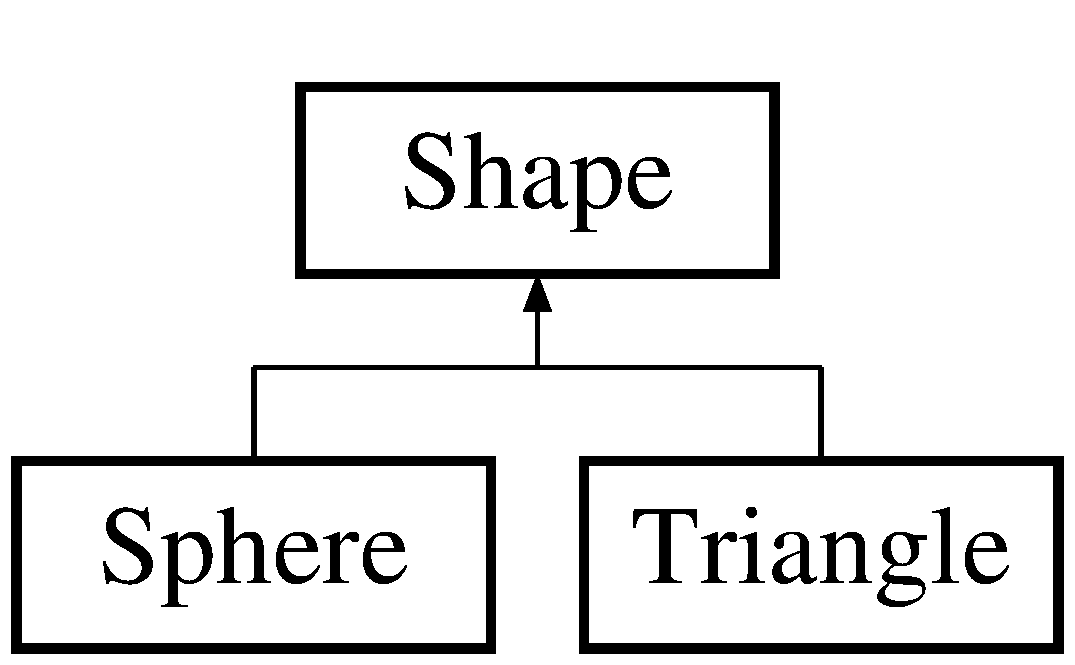
\includegraphics[height=2.000000cm]{class_shape}
\end{center}
\end{figure}
\subsection*{Public Member Functions}
\begin{DoxyCompactItemize}
\item 
virtual bool \mbox{\hyperlink{class_shape_a06081ad5df190daf858f295bd8e8a0e1}{intersect}} (\mbox{\hyperlink{class_ray}{Ray}} \&ray, \mbox{\hyperlink{class_intersection}{Intersection}} \&intersection, bool cull\+Back)
\item 
virtual bool \mbox{\hyperlink{class_shape_a41cb78dcc1b919cdba2b7fbc0a1a0bc8}{intersect}} (\mbox{\hyperlink{class_ray}{Ray}} \&ray, bool cull\+Back)
\item 
\mbox{\Hypertarget{class_shape_ad4f344dbda0fb8446805631c0c408a16}\label{class_shape_ad4f344dbda0fb8446805631c0c408a16}} 
virtual bool \mbox{\hyperlink{class_shape_ad4f344dbda0fb8446805631c0c408a16}{pretransform}} (\mbox{\hyperlink{class_transform}{Transform}} \&obj2world)
\begin{DoxyCompactList}\small\item\em Test intersection between shape and ray. \end{DoxyCompactList}\item 
\mbox{\Hypertarget{class_shape_ac988eb692cfbfcaa1907491938a55b7a}\label{class_shape_ac988eb692cfbfcaa1907491938a55b7a}} 
virtual bool \mbox{\hyperlink{class_shape_ac988eb692cfbfcaa1907491938a55b7a}{is\+Front}} (const \mbox{\hyperlink{struct_vector}{Vector}} \&dir)
\begin{DoxyCompactList}\small\item\em Test if ray hit front side of shape. \end{DoxyCompactList}\end{DoxyCompactItemize}


\subsection{Detailed Description}
\mbox{\hyperlink{class_shape}{Shape}}

Methods\+:

Test if ray intersects with the shape or not (in object space), if so, return intersection point and normal

bool intersect(\+Ray\& ray, float$\ast$ thit, Local\+Geo$\ast$ local)

Same as intersect, but just return whether there is any intersection or not

bool intersect\+P(\+Ray\& ray)

Notes\+: \mbox{\hyperlink{class_triangle}{Triangle}} and \mbox{\hyperlink{class_sphere}{Sphere}} are probably best implemented here The intersection with the ray at t outside the range \mbox{[}t\+\_\+min, t\+\_\+max\mbox{]} should return false. 

\subsection{Member Function Documentation}
\mbox{\Hypertarget{class_shape_a06081ad5df190daf858f295bd8e8a0e1}\label{class_shape_a06081ad5df190daf858f295bd8e8a0e1}} 
\index{Shape@{Shape}!intersect@{intersect}}
\index{intersect@{intersect}!Shape@{Shape}}
\subsubsection{\texorpdfstring{intersect()}{intersect()}\hspace{0.1cm}{\footnotesize\ttfamily [1/2]}}
{\footnotesize\ttfamily virtual bool Shape\+::intersect (\begin{DoxyParamCaption}\item[{\mbox{\hyperlink{class_ray}{Ray}} \&}]{ray,  }\item[{\mbox{\hyperlink{class_intersection}{Intersection}} \&}]{intersection,  }\item[{bool}]{cull\+Back }\end{DoxyParamCaption})\hspace{0.3cm}{\ttfamily [inline]}, {\ttfamily [virtual]}}

Test intersection between shape and ray 
\begin{DoxyParams}[1]{Parameters}
 & {\em ray} & \\
\hline
\mbox{\tt in,out}  & {\em in} & intersection \\
\hline
 & {\em cull} & back face culling \\
\hline
\end{DoxyParams}
\begin{DoxyReturn}{Returns}
true for sucessfull intersection 
\end{DoxyReturn}


Reimplemented in \mbox{\hyperlink{class_triangle_ad78a148da18386f99f23731ce7de431f}{Triangle}}, and \mbox{\hyperlink{class_sphere_ab4700cd65d2bba22863d0bee673e8bf3}{Sphere}}.

\mbox{\Hypertarget{class_shape_a41cb78dcc1b919cdba2b7fbc0a1a0bc8}\label{class_shape_a41cb78dcc1b919cdba2b7fbc0a1a0bc8}} 
\index{Shape@{Shape}!intersect@{intersect}}
\index{intersect@{intersect}!Shape@{Shape}}
\subsubsection{\texorpdfstring{intersect()}{intersect()}\hspace{0.1cm}{\footnotesize\ttfamily [2/2]}}
{\footnotesize\ttfamily virtual bool Shape\+::intersect (\begin{DoxyParamCaption}\item[{\mbox{\hyperlink{class_ray}{Ray}} \&}]{ray,  }\item[{bool}]{cull\+Back }\end{DoxyParamCaption})\hspace{0.3cm}{\ttfamily [inline]}, {\ttfamily [virtual]}}

Test intersection between shape and ray 
\begin{DoxyParams}{Parameters}
{\em ray} & \\
\hline
{\em cull} & back face culling \\
\hline
\end{DoxyParams}
\begin{DoxyReturn}{Returns}
true for sucessfull intersection 
\end{DoxyReturn}


Reimplemented in \mbox{\hyperlink{class_triangle_abf8edc617d32e7c651a01efc0cb4647e}{Triangle}}, and \mbox{\hyperlink{class_sphere_a0ca2b62d692108272b9b64857965838b}{Sphere}}.



The documentation for this class was generated from the following file\+:\begin{DoxyCompactItemize}
\item 
\mbox{\hyperlink{shape_8h}{shape.\+h}}\end{DoxyCompactItemize}

\hypertarget{class_sphere}{}\section{Sphere Class Reference}
\label{class_sphere}\index{Sphere@{Sphere}}


{\ttfamily \#include $<$sphere.\+h$>$}

Inheritance diagram for Sphere\+:\begin{figure}[H]
\begin{center}
\leavevmode
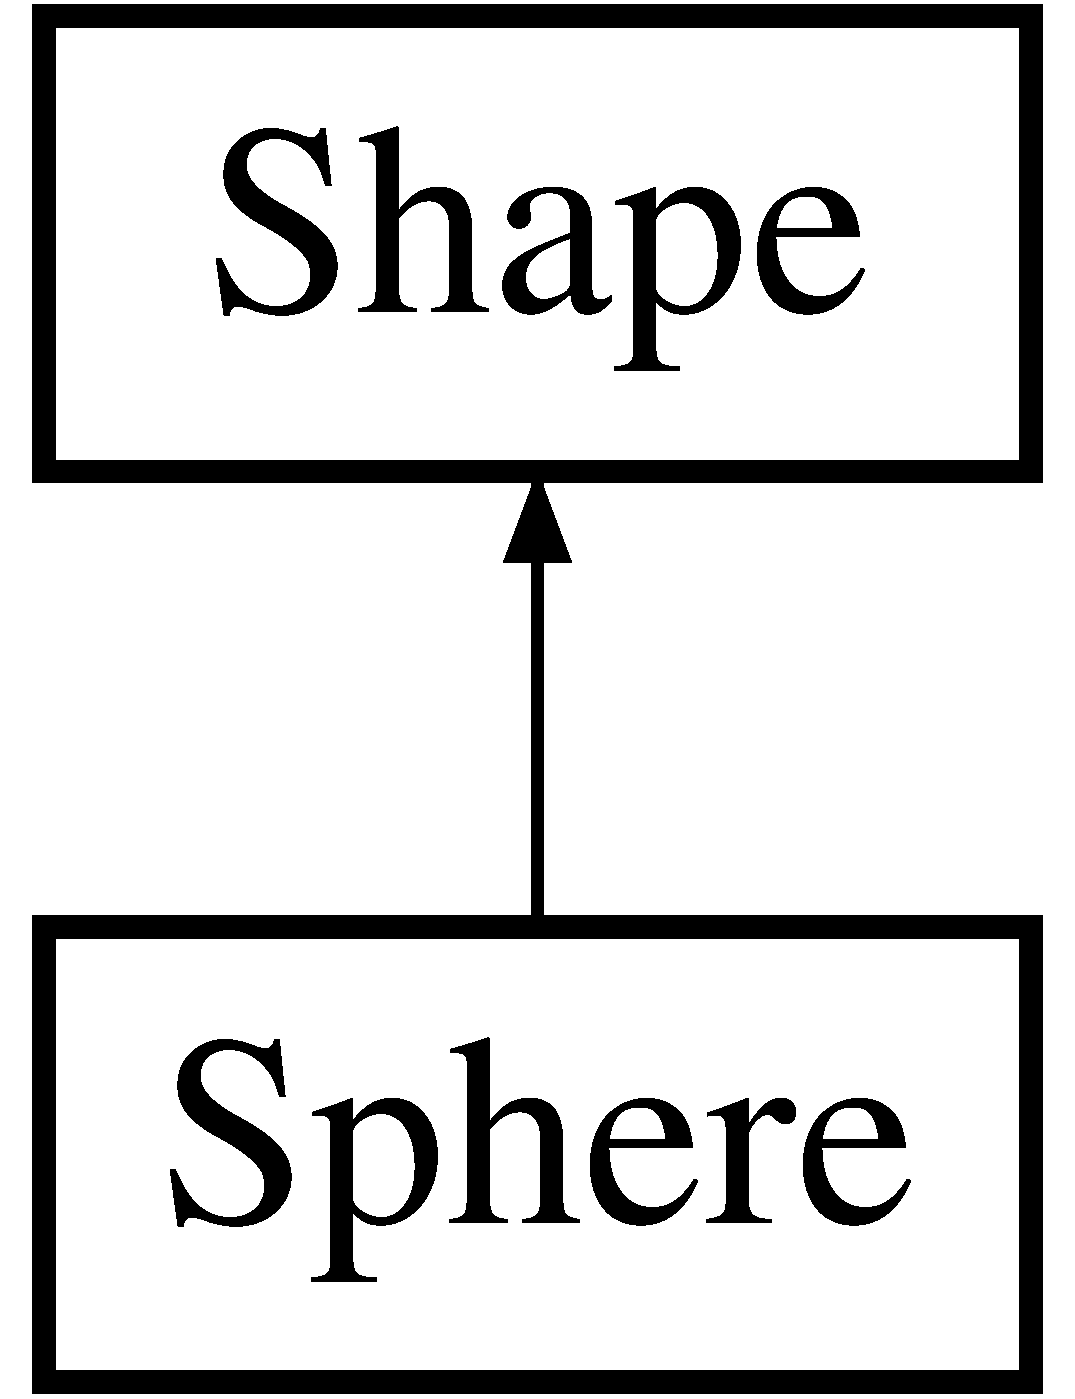
\includegraphics[height=2.000000cm]{class_sphere}
\end{center}
\end{figure}
\subsection*{Public Member Functions}
\begin{DoxyCompactItemize}
\item 
\mbox{\hyperlink{class_sphere_acdc6a785051367320ea2fbbb66769b1a}{Sphere}} (const \mbox{\hyperlink{struct_vector}{Vector}} \&pos, float rad)
\item 
bool \mbox{\hyperlink{class_sphere_ab4700cd65d2bba22863d0bee673e8bf3}{intersect}} (\mbox{\hyperlink{class_ray}{Ray}} \&ray, \mbox{\hyperlink{class_intersection}{Intersection}} \&intersection, bool cull\+Back)
\item 
bool \mbox{\hyperlink{class_sphere_a0ca2b62d692108272b9b64857965838b}{intersect}} (\mbox{\hyperlink{class_ray}{Ray}} \&ray, bool cull\+Back)
\end{DoxyCompactItemize}
\subsection*{Public Attributes}
\begin{DoxyCompactItemize}
\item 
\mbox{\Hypertarget{class_sphere_ad8604838ba9a34188843f422afdc7a8e}\label{class_sphere_ad8604838ba9a34188843f422afdc7a8e}} 
\mbox{\hyperlink{struct_vector}{Vector}} \mbox{\hyperlink{class_sphere_ad8604838ba9a34188843f422afdc7a8e}{center}}
\begin{DoxyCompactList}\small\item\em \mbox{\hyperlink{class_sphere}{Sphere}} center position. \end{DoxyCompactList}\item 
\mbox{\Hypertarget{class_sphere_ae6f42f0da6679a2f0b4a22681ccccf38}\label{class_sphere_ae6f42f0da6679a2f0b4a22681ccccf38}} 
float \mbox{\hyperlink{class_sphere_ae6f42f0da6679a2f0b4a22681ccccf38}{radius}}
\begin{DoxyCompactList}\small\item\em \mbox{\hyperlink{class_sphere}{Sphere}}\textquotesingle{}s radius. \end{DoxyCompactList}\end{DoxyCompactItemize}


\subsection{Detailed Description}
\mbox{\hyperlink{class_sphere}{Sphere}} primitive

Fields\+: center position radius 

\subsection{Constructor \& Destructor Documentation}
\mbox{\Hypertarget{class_sphere_acdc6a785051367320ea2fbbb66769b1a}\label{class_sphere_acdc6a785051367320ea2fbbb66769b1a}} 
\index{Sphere@{Sphere}!Sphere@{Sphere}}
\index{Sphere@{Sphere}!Sphere@{Sphere}}
\subsubsection{\texorpdfstring{Sphere()}{Sphere()}}
{\footnotesize\ttfamily Sphere\+::\+Sphere (\begin{DoxyParamCaption}\item[{const \mbox{\hyperlink{struct_vector}{Vector}} \&}]{pos,  }\item[{float}]{rad }\end{DoxyParamCaption})\hspace{0.3cm}{\ttfamily [inline]}}

Construct sphere 
\begin{DoxyParams}{Parameters}
{\em pos} & position of center \\
\hline
{\em rad} & sphere radius \\
\hline
\end{DoxyParams}


\subsection{Member Function Documentation}
\mbox{\Hypertarget{class_sphere_ab4700cd65d2bba22863d0bee673e8bf3}\label{class_sphere_ab4700cd65d2bba22863d0bee673e8bf3}} 
\index{Sphere@{Sphere}!intersect@{intersect}}
\index{intersect@{intersect}!Sphere@{Sphere}}
\subsubsection{\texorpdfstring{intersect()}{intersect()}\hspace{0.1cm}{\footnotesize\ttfamily [1/2]}}
{\footnotesize\ttfamily bool Sphere\+::intersect (\begin{DoxyParamCaption}\item[{\mbox{\hyperlink{class_ray}{Ray}} \&}]{ray,  }\item[{\mbox{\hyperlink{class_intersection}{Intersection}} \&}]{intersection,  }\item[{bool}]{cull\+Back }\end{DoxyParamCaption})\hspace{0.3cm}{\ttfamily [inline]}, {\ttfamily [virtual]}}

Test intersection between sphere and ray 
\begin{DoxyParams}[1]{Parameters}
 & {\em ray} & \\
\hline
\mbox{\tt in,out}  & {\em o\+Intersect} & intersection \\
\hline
 & {\em cull\+Back} & to cull back face culling (not used) \\
\hline
\end{DoxyParams}
\begin{DoxyReturn}{Returns}
true for sucessful intersections 
\end{DoxyReturn}


Reimplemented from \mbox{\hyperlink{class_shape_a06081ad5df190daf858f295bd8e8a0e1}{Shape}}.

\mbox{\Hypertarget{class_sphere_a0ca2b62d692108272b9b64857965838b}\label{class_sphere_a0ca2b62d692108272b9b64857965838b}} 
\index{Sphere@{Sphere}!intersect@{intersect}}
\index{intersect@{intersect}!Sphere@{Sphere}}
\subsubsection{\texorpdfstring{intersect()}{intersect()}\hspace{0.1cm}{\footnotesize\ttfamily [2/2]}}
{\footnotesize\ttfamily bool Sphere\+::intersect (\begin{DoxyParamCaption}\item[{\mbox{\hyperlink{class_ray}{Ray}} \&}]{ray,  }\item[{bool}]{cull\+Back }\end{DoxyParamCaption})\hspace{0.3cm}{\ttfamily [inline]}, {\ttfamily [virtual]}}

Test intersection between sphere and ray 
\begin{DoxyParams}{Parameters}
{\em ray} & \\
\hline
{\em cull\+Back} & to cull back face culling (not used) \\
\hline
\end{DoxyParams}
\begin{DoxyReturn}{Returns}
true for sucessful intersections 
\end{DoxyReturn}


Reimplemented from \mbox{\hyperlink{class_shape_a41cb78dcc1b919cdba2b7fbc0a1a0bc8}{Shape}}.



The documentation for this class was generated from the following file\+:\begin{DoxyCompactItemize}
\item 
\mbox{\hyperlink{sphere_8h}{sphere.\+h}}\end{DoxyCompactItemize}

\hypertarget{class_surface_point}{}\section{Surface\+Point Class Reference}
\label{class_surface_point}\index{Surface\+Point@{Surface\+Point}}


{\ttfamily \#include $<$surface\+\_\+point.\+h$>$}

\subsection*{Public Attributes}
\begin{DoxyCompactItemize}
\item 
\mbox{\Hypertarget{class_surface_point_a08f317429035a1cc8b52646d472451a3}\label{class_surface_point_a08f317429035a1cc8b52646d472451a3}} 
\mbox{\hyperlink{struct_vector}{Vector}} {\bfseries position}
\item 
\mbox{\Hypertarget{class_surface_point_ac7064733be92b5cc4b8d68ce63d65bf1}\label{class_surface_point_ac7064733be92b5cc4b8d68ce63d65bf1}} 
\mbox{\hyperlink{struct_vector}{Vector}} {\bfseries normal}
\end{DoxyCompactItemize}


\subsection{Detailed Description}
\mbox{\hyperlink{class_surface_point}{Surface\+Point}} Contains the collision information between ray and geometry or primitive

Members\+: Point pos Normal normal

Notes\+: Store the local geometry at the intersection point. To\+Do\+: May need to store other quantities (eg. texture coordinate) in a more complicated raytracer. 

The documentation for this class was generated from the following file\+:\begin{DoxyCompactItemize}
\item 
surface\+\_\+point.\+h\end{DoxyCompactItemize}

\hypertarget{class_transform}{}\section{Transform Class Reference}
\label{class_transform}\index{Transform@{Transform}}


{\ttfamily \#include $<$transform.\+h$>$}

\subsection*{Public Member Functions}
\begin{DoxyCompactItemize}
\item 
\mbox{\Hypertarget{class_transform_aa08ca4266efabc768973cdeea51945ab}\label{class_transform_aa08ca4266efabc768973cdeea51945ab}} 
\mbox{\hyperlink{class_transform_aa08ca4266efabc768973cdeea51945ab}{Transform}} ()
\begin{DoxyCompactList}\small\item\em Construct default transform matrix. \end{DoxyCompactList}\item 
\mbox{\hyperlink{class_transform_a9e66877ba4b108deb475d91b3e484b19}{Transform}} (mat4 m)
\item 
void \mbox{\hyperlink{class_transform_a527516549fad2a69271d82935e42e409}{set\+Transformation}} (mat4 m\+\_\+)
\item 
\mbox{\hyperlink{struct_vector}{Vector}} \mbox{\hyperlink{class_transform_a0326d611d8d74b4a43f0b6aaf1b87d67}{transform}} (\mbox{\hyperlink{struct_vector}{Vector}} v)
\item 
void \mbox{\hyperlink{class_transform_a9e08226abcc24477177fe1eeafaa43df}{transform}} (\mbox{\hyperlink{class_ray}{Ray}} \&ray)
\item 
void \mbox{\hyperlink{class_transform_afd54e58d092b30f7613f86c68a43ea9a}{transform}} (\mbox{\hyperlink{class_surface_point}{Surface\+Point}} \&surf\+Point)
\end{DoxyCompactItemize}
\subsection*{Static Public Member Functions}
\begin{DoxyCompactItemize}
\item 
static mat4 \mbox{\hyperlink{class_transform_a846e6b2bec58a1110d4e5296b1caa1f4}{look\+At}} (const vec3 \&cam\+Position, const vec3 \&targ\+Position, const vec3 \&up)
\item 
static mat4 \mbox{\hyperlink{class_transform_a2045e6a0d6071568fa8a2d3819a52dc7}{perspective}} (float fovy, float aspect, float near, float far)
\item 
static mat3 \mbox{\hyperlink{class_transform_a41cee512b56644e2bf87d82a26adbe01}{rotate}} (const vec3 \&axis, const float angle)
\item 
static mat4 \mbox{\hyperlink{class_transform_a8c96f4dcc6aee87b1a2b66b9fbdbfc7c}{scale}} (const float \&sx, const float \&sy, const float \&sz)
\item 
static mat4 \mbox{\hyperlink{class_transform_aee43231752c8d0f5133b0374007252a2}{translate}} (const float \&tx, const float \&ty, const float \&tz)
\end{DoxyCompactItemize}
\subsection*{Public Attributes}
\begin{DoxyCompactItemize}
\item 
\mbox{\Hypertarget{class_transform_ac7c371bdd14ff1c6434cac58082eff10}\label{class_transform_ac7c371bdd14ff1c6434cac58082eff10}} 
mat4 {\bfseries m}
\item 
\mbox{\Hypertarget{class_transform_a57f1d2c66d7715757bbd79c61774dd87}\label{class_transform_a57f1d2c66d7715757bbd79c61774dd87}} 
mat4 {\bfseries minvt}
\end{DoxyCompactItemize}


\subsection{Detailed Description}
Contains matrix \textquotesingle{}m\textquotesingle{} and its inverse vversion \textquotesingle{}minvt\textquotesingle{} (for transforming normals) 

\subsection{Constructor \& Destructor Documentation}
\mbox{\Hypertarget{class_transform_a9e66877ba4b108deb475d91b3e484b19}\label{class_transform_a9e66877ba4b108deb475d91b3e484b19}} 
\index{Transform@{Transform}!Transform@{Transform}}
\index{Transform@{Transform}!Transform@{Transform}}
\subsubsection{\texorpdfstring{Transform()}{Transform()}}
{\footnotesize\ttfamily Transform\+::\+Transform (\begin{DoxyParamCaption}\item[{mat4}]{m }\end{DoxyParamCaption})\hspace{0.3cm}{\ttfamily [inline]}}

Construct transform from given matrix 
\begin{DoxyParams}{Parameters}
{\em m} & the transformation matrix \\
\hline
\end{DoxyParams}


\subsection{Member Function Documentation}
\mbox{\Hypertarget{class_transform_a846e6b2bec58a1110d4e5296b1caa1f4}\label{class_transform_a846e6b2bec58a1110d4e5296b1caa1f4}} 
\index{Transform@{Transform}!look\+At@{look\+At}}
\index{look\+At@{look\+At}!Transform@{Transform}}
\subsubsection{\texorpdfstring{look\+At()}{lookAt()}}
{\footnotesize\ttfamily mat4 Transform\+::look\+At (\begin{DoxyParamCaption}\item[{const vec3 \&}]{cam\+Position,  }\item[{const vec3 \&}]{targ\+Position,  }\item[{const vec3 \&}]{up }\end{DoxyParamCaption})\hspace{0.3cm}{\ttfamily [static]}}

Create look at matrix 
\begin{DoxyParams}{Parameters}
{\em cam\+Position} & camera position \\
\hline
{\em targ\+Position} & target point position \\
\hline
{\em up} & desired up vector \\
\hline
\end{DoxyParams}
\mbox{\Hypertarget{class_transform_a2045e6a0d6071568fa8a2d3819a52dc7}\label{class_transform_a2045e6a0d6071568fa8a2d3819a52dc7}} 
\index{Transform@{Transform}!perspective@{perspective}}
\index{perspective@{perspective}!Transform@{Transform}}
\subsubsection{\texorpdfstring{perspective()}{perspective()}}
{\footnotesize\ttfamily mat4 Transform\+::perspective (\begin{DoxyParamCaption}\item[{float}]{fovy,  }\item[{float}]{aspect,  }\item[{float}]{near,  }\item[{float}]{far }\end{DoxyParamCaption})\hspace{0.3cm}{\ttfamily [static]}}

Create perspective matrix 
\begin{DoxyParams}{Parameters}
{\em fovy} & vertical field of view \\
\hline
{\em aspect} & the aspect ratio \\
\hline
{\em near} & plane \\
\hline
{\em far} & plane \\
\hline
\end{DoxyParams}
\mbox{\Hypertarget{class_transform_a41cee512b56644e2bf87d82a26adbe01}\label{class_transform_a41cee512b56644e2bf87d82a26adbe01}} 
\index{Transform@{Transform}!rotate@{rotate}}
\index{rotate@{rotate}!Transform@{Transform}}
\subsubsection{\texorpdfstring{rotate()}{rotate()}}
{\footnotesize\ttfamily mat3 Transform\+::rotate (\begin{DoxyParamCaption}\item[{const vec3 \&}]{axis,  }\item[{const float}]{angle }\end{DoxyParamCaption})\hspace{0.3cm}{\ttfamily [static]}}

Create rotation matrix 
\begin{DoxyParams}{Parameters}
{\em angle} & the rotation angle \\
\hline
{\em axis} & trotate aroutd this axis \\
\hline
\end{DoxyParams}
\mbox{\Hypertarget{class_transform_a8c96f4dcc6aee87b1a2b66b9fbdbfc7c}\label{class_transform_a8c96f4dcc6aee87b1a2b66b9fbdbfc7c}} 
\index{Transform@{Transform}!scale@{scale}}
\index{scale@{scale}!Transform@{Transform}}
\subsubsection{\texorpdfstring{scale()}{scale()}}
{\footnotesize\ttfamily mat4 Transform\+::scale (\begin{DoxyParamCaption}\item[{const float \&}]{sx,  }\item[{const float \&}]{sy,  }\item[{const float \&}]{sz }\end{DoxyParamCaption})\hspace{0.3cm}{\ttfamily [static]}}

Create scale matrix 
\begin{DoxyParams}{Parameters}
{\em sx} & scale \\
\hline
{\em sy} & scale \\
\hline
{\em sz} & scale \\
\hline
\end{DoxyParams}
\mbox{\Hypertarget{class_transform_a527516549fad2a69271d82935e42e409}\label{class_transform_a527516549fad2a69271d82935e42e409}} 
\index{Transform@{Transform}!set\+Transformation@{set\+Transformation}}
\index{set\+Transformation@{set\+Transformation}!Transform@{Transform}}
\subsubsection{\texorpdfstring{set\+Transformation()}{setTransformation()}}
{\footnotesize\ttfamily void Transform\+::set\+Transformation (\begin{DoxyParamCaption}\item[{mat4}]{m\+\_\+ }\end{DoxyParamCaption})\hspace{0.3cm}{\ttfamily [inline]}}

Set transform to given matrix  m\+\_\+ new transformation matrix \mbox{\Hypertarget{class_transform_a0326d611d8d74b4a43f0b6aaf1b87d67}\label{class_transform_a0326d611d8d74b4a43f0b6aaf1b87d67}} 
\index{Transform@{Transform}!transform@{transform}}
\index{transform@{transform}!Transform@{Transform}}
\subsubsection{\texorpdfstring{transform()}{transform()}\hspace{0.1cm}{\footnotesize\ttfamily [1/3]}}
{\footnotesize\ttfamily \mbox{\hyperlink{struct_vector}{Vector}} Transform\+::transform (\begin{DoxyParamCaption}\item[{\mbox{\hyperlink{struct_vector}{Vector}}}]{v }\end{DoxyParamCaption})}

\mbox{\hyperlink{class_transform}{Transform}} vector  v input vector \begin{DoxyReturn}{Returns}
is transformed vector 
\end{DoxyReturn}
\mbox{\Hypertarget{class_transform_a9e08226abcc24477177fe1eeafaa43df}\label{class_transform_a9e08226abcc24477177fe1eeafaa43df}} 
\index{Transform@{Transform}!transform@{transform}}
\index{transform@{transform}!Transform@{Transform}}
\subsubsection{\texorpdfstring{transform()}{transform()}\hspace{0.1cm}{\footnotesize\ttfamily [2/3]}}
{\footnotesize\ttfamily void Transform\+::transform (\begin{DoxyParamCaption}\item[{\mbox{\hyperlink{class_ray}{Ray}} \&}]{ray }\end{DoxyParamCaption})}

\mbox{\hyperlink{class_transform}{Transform}} ray 
\begin{DoxyParams}[1]{Parameters}
\mbox{\tt in,out}  & {\em ray} & will be updated \\
\hline
\end{DoxyParams}
\mbox{\Hypertarget{class_transform_afd54e58d092b30f7613f86c68a43ea9a}\label{class_transform_afd54e58d092b30f7613f86c68a43ea9a}} 
\index{Transform@{Transform}!transform@{transform}}
\index{transform@{transform}!Transform@{Transform}}
\subsubsection{\texorpdfstring{transform()}{transform()}\hspace{0.1cm}{\footnotesize\ttfamily [3/3]}}
{\footnotesize\ttfamily void Transform\+::transform (\begin{DoxyParamCaption}\item[{\mbox{\hyperlink{class_surface_point}{Surface\+Point}} \&}]{surf\+Point }\end{DoxyParamCaption})}

\mbox{\hyperlink{class_transform}{Transform}} geometry 
\begin{DoxyParams}[1]{Parameters}
\mbox{\tt in,out}  & {\em ray} & will be updated \\
\hline
\end{DoxyParams}
\mbox{\Hypertarget{class_transform_aee43231752c8d0f5133b0374007252a2}\label{class_transform_aee43231752c8d0f5133b0374007252a2}} 
\index{Transform@{Transform}!translate@{translate}}
\index{translate@{translate}!Transform@{Transform}}
\subsubsection{\texorpdfstring{translate()}{translate()}}
{\footnotesize\ttfamily mat4 Transform\+::translate (\begin{DoxyParamCaption}\item[{const float \&}]{tx,  }\item[{const float \&}]{ty,  }\item[{const float \&}]{tz }\end{DoxyParamCaption})\hspace{0.3cm}{\ttfamily [static]}}

Create translation matrix 
\begin{DoxyParams}{Parameters}
{\em tx} & translate position \\
\hline
{\em ty} & translate position \\
\hline
{\em tz} & translate position \\
\hline
\end{DoxyParams}


The documentation for this class was generated from the following files\+:\begin{DoxyCompactItemize}
\item 
\mbox{\hyperlink{transform_8h}{transform.\+h}}\item 
\mbox{\hyperlink{transform_8cpp}{transform.\+cpp}}\end{DoxyCompactItemize}

\hypertarget{class_triangle}{}\section{Triangle Class Reference}
\label{class_triangle}\index{Triangle@{Triangle}}


Cointans three world position and thre bormals normal. Additionaly contans normal for triangle.  




{\ttfamily \#include $<$triangle.\+h$>$}

Inheritance diagram for Triangle\+:\begin{figure}[H]
\begin{center}
\leavevmode
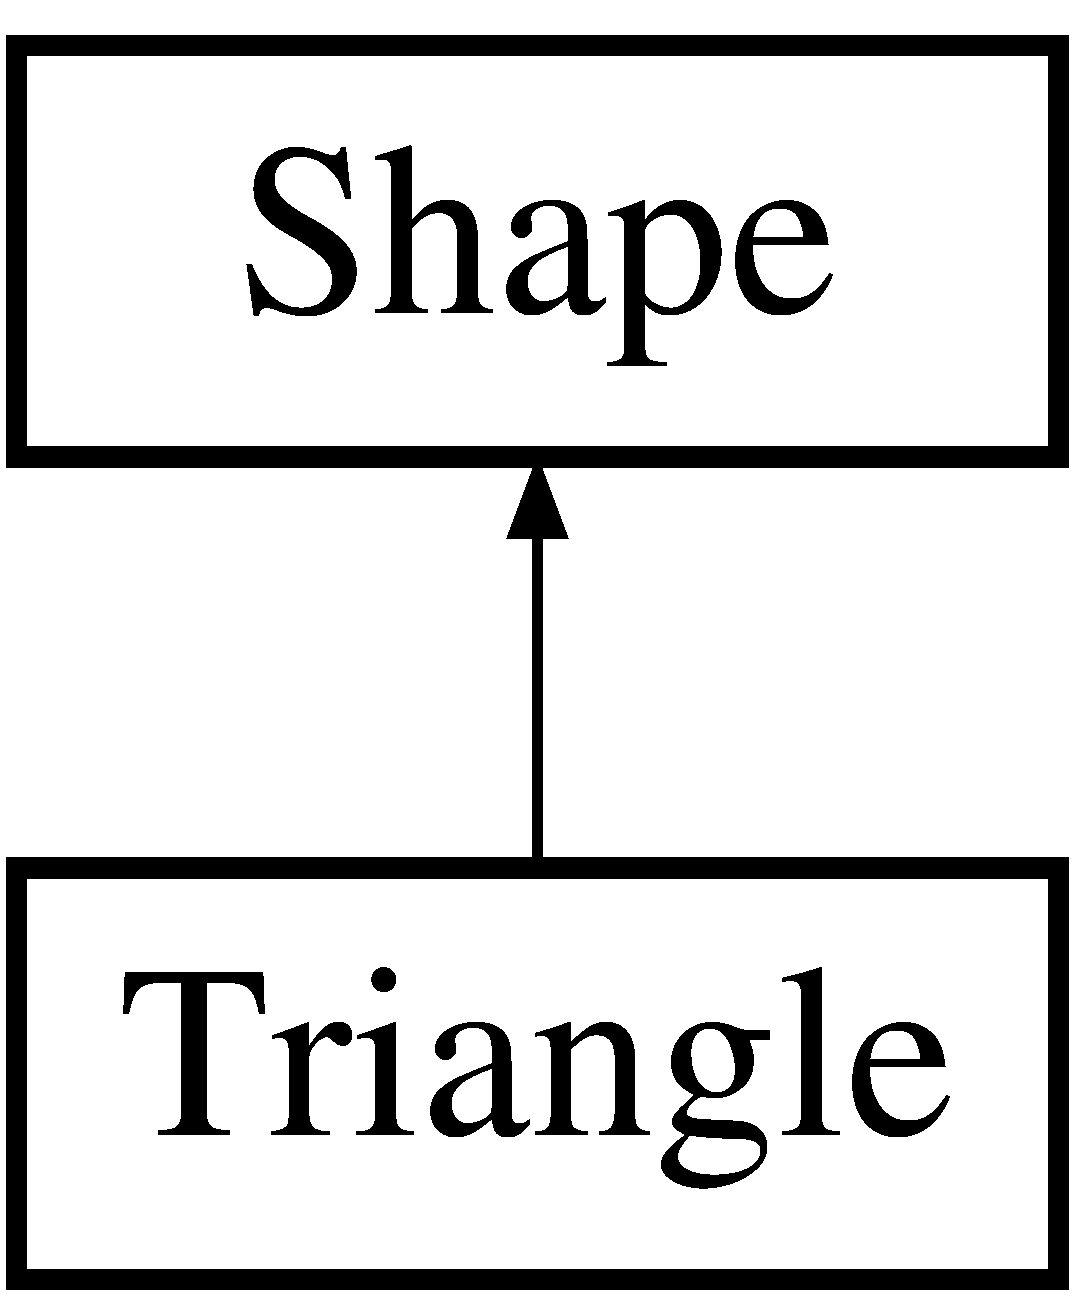
\includegraphics[height=2.000000cm]{class_triangle}
\end{center}
\end{figure}
\subsection*{Public Member Functions}
\begin{DoxyCompactItemize}
\item 
\mbox{\hyperlink{class_triangle_a903d25822fb5103ea3dcb03efa0cea2a}{Triangle}} (\mbox{\hyperlink{struct_vector}{Vector}} v1, \mbox{\hyperlink{struct_vector}{Vector}} v2, \mbox{\hyperlink{struct_vector}{Vector}} v3)
\item 
\mbox{\hyperlink{class_triangle_a54140a599b11aa207d2dd46369ff94b4}{Triangle}} (\mbox{\hyperlink{struct_vector}{Vector}} v1, \mbox{\hyperlink{struct_vector}{Vector}} v2, \mbox{\hyperlink{struct_vector}{Vector}} v3, \mbox{\hyperlink{struct_vector}{Vector}} n1, \mbox{\hyperlink{struct_vector}{Vector}} n2, \mbox{\hyperlink{struct_vector}{Vector}} n3)
\item 
bool \mbox{\hyperlink{class_triangle_ad78a148da18386f99f23731ce7de431f}{intersect}} (\mbox{\hyperlink{class_ray}{Ray}} \&ray, \mbox{\hyperlink{class_intersection}{Intersection}} \&intersection, bool cull\+Back)
\item 
bool \mbox{\hyperlink{class_triangle_abf8edc617d32e7c651a01efc0cb4647e}{intersect}} (\mbox{\hyperlink{class_ray}{Ray}} \&ray, bool cull\+Back)
\item 
virtual bool \mbox{\hyperlink{class_triangle_a8fef25a36bfe124a5e632e4f9fe2726f}{pretransform}} (\mbox{\hyperlink{class_transform}{Transform}} \&obj2world)
\item 
virtual bool \mbox{\hyperlink{class_triangle_a3c33c1eb1d04b85a40426d3a14819d74}{is\+Front}} (const \mbox{\hyperlink{struct_vector}{Vector}} \&dir)
\end{DoxyCompactItemize}


\subsection{Detailed Description}
Cointans three world position and thre bormals normal. Additionaly contans normal for triangle. 

\subsection{Constructor \& Destructor Documentation}
\mbox{\Hypertarget{class_triangle_a903d25822fb5103ea3dcb03efa0cea2a}\label{class_triangle_a903d25822fb5103ea3dcb03efa0cea2a}} 
\index{Triangle@{Triangle}!Triangle@{Triangle}}
\index{Triangle@{Triangle}!Triangle@{Triangle}}
\subsubsection{\texorpdfstring{Triangle()}{Triangle()}\hspace{0.1cm}{\footnotesize\ttfamily [1/2]}}
{\footnotesize\ttfamily Triangle\+::\+Triangle (\begin{DoxyParamCaption}\item[{\mbox{\hyperlink{struct_vector}{Vector}}}]{v1,  }\item[{\mbox{\hyperlink{struct_vector}{Vector}}}]{v2,  }\item[{\mbox{\hyperlink{struct_vector}{Vector}}}]{v3 }\end{DoxyParamCaption})\hspace{0.3cm}{\ttfamily [inline]}}

Construct planar triangle 
\begin{DoxyParams}{Parameters}
{\em v1} & point one \\
\hline
{\em v2} & point two \\
\hline
{\em v3} & point three \\
\hline
\end{DoxyParams}
\mbox{\Hypertarget{class_triangle_a54140a599b11aa207d2dd46369ff94b4}\label{class_triangle_a54140a599b11aa207d2dd46369ff94b4}} 
\index{Triangle@{Triangle}!Triangle@{Triangle}}
\index{Triangle@{Triangle}!Triangle@{Triangle}}
\subsubsection{\texorpdfstring{Triangle()}{Triangle()}\hspace{0.1cm}{\footnotesize\ttfamily [2/2]}}
{\footnotesize\ttfamily Triangle\+::\+Triangle (\begin{DoxyParamCaption}\item[{\mbox{\hyperlink{struct_vector}{Vector}}}]{v1,  }\item[{\mbox{\hyperlink{struct_vector}{Vector}}}]{v2,  }\item[{\mbox{\hyperlink{struct_vector}{Vector}}}]{v3,  }\item[{\mbox{\hyperlink{struct_vector}{Vector}}}]{n1,  }\item[{\mbox{\hyperlink{struct_vector}{Vector}}}]{n2,  }\item[{\mbox{\hyperlink{struct_vector}{Vector}}}]{n3 }\end{DoxyParamCaption})\hspace{0.3cm}{\ttfamily [inline]}}

Construct non planar triangle 
\begin{DoxyParams}{Parameters}
{\em v1} & point one \\
\hline
{\em v2} & point two \\
\hline
{\em v3} & point three \\
\hline
{\em n1} & normal one \\
\hline
{\em n2} & normal two \\
\hline
{\em n3} & normal three \\
\hline
\end{DoxyParams}


\subsection{Member Function Documentation}
\mbox{\Hypertarget{class_triangle_ad78a148da18386f99f23731ce7de431f}\label{class_triangle_ad78a148da18386f99f23731ce7de431f}} 
\index{Triangle@{Triangle}!intersect@{intersect}}
\index{intersect@{intersect}!Triangle@{Triangle}}
\subsubsection{\texorpdfstring{intersect()}{intersect()}\hspace{0.1cm}{\footnotesize\ttfamily [1/2]}}
{\footnotesize\ttfamily bool Triangle\+::intersect (\begin{DoxyParamCaption}\item[{\mbox{\hyperlink{class_ray}{Ray}} \&}]{ray,  }\item[{\mbox{\hyperlink{class_intersection}{Intersection}} \&}]{intersection,  }\item[{bool}]{cull\+Back }\end{DoxyParamCaption})\hspace{0.3cm}{\ttfamily [inline]}, {\ttfamily [virtual]}}

Test intersection between this triangle and ray. 
\begin{DoxyParams}[1]{Parameters}
 & {\em ray} & \\
\hline
\mbox{\tt out}  & {\em intersection} & \mbox{\hyperlink{class_intersection}{Intersection}} \\
\hline
 & {\em cull\+Back} & In case if it is true then ignore back side of triangle \\
\hline
\end{DoxyParams}
\begin{DoxyReturn}{Returns}
true for sucessful intersection 
\end{DoxyReturn}


Reimplemented from \mbox{\hyperlink{class_shape_a06081ad5df190daf858f295bd8e8a0e1}{Shape}}.

\mbox{\Hypertarget{class_triangle_abf8edc617d32e7c651a01efc0cb4647e}\label{class_triangle_abf8edc617d32e7c651a01efc0cb4647e}} 
\index{Triangle@{Triangle}!intersect@{intersect}}
\index{intersect@{intersect}!Triangle@{Triangle}}
\subsubsection{\texorpdfstring{intersect()}{intersect()}\hspace{0.1cm}{\footnotesize\ttfamily [2/2]}}
{\footnotesize\ttfamily bool Triangle\+::intersect (\begin{DoxyParamCaption}\item[{\mbox{\hyperlink{class_ray}{Ray}} \&}]{ray,  }\item[{bool}]{cull\+Back }\end{DoxyParamCaption})\hspace{0.3cm}{\ttfamily [inline]}, {\ttfamily [virtual]}}

Test intersection between this triangle and ray. 
\begin{DoxyParams}{Parameters}
{\em ray} & the ray to intersect \\
\hline
{\em cull\+Back} & In case if it is true then ignore back side of triangle \\
\hline
\end{DoxyParams}
\begin{DoxyReturn}{Returns}
true for sucessful intersection 
\end{DoxyReturn}


Reimplemented from \mbox{\hyperlink{class_shape_a41cb78dcc1b919cdba2b7fbc0a1a0bc8}{Shape}}.

\mbox{\Hypertarget{class_triangle_a3c33c1eb1d04b85a40426d3a14819d74}\label{class_triangle_a3c33c1eb1d04b85a40426d3a14819d74}} 
\index{Triangle@{Triangle}!is\+Front@{is\+Front}}
\index{is\+Front@{is\+Front}!Triangle@{Triangle}}
\subsubsection{\texorpdfstring{is\+Front()}{isFront()}}
{\footnotesize\ttfamily virtual bool Triangle\+::is\+Front (\begin{DoxyParamCaption}\item[{const \mbox{\hyperlink{struct_vector}{Vector}} \&}]{dir }\end{DoxyParamCaption})\hspace{0.3cm}{\ttfamily [inline]}, {\ttfamily [virtual]}}

Test if light ray\textquotesingle{}s direction hit fron face of this triangle 
\begin{DoxyParams}{Parameters}
{\em dir} & the light\textquotesingle{}s direction \\
\hline
\end{DoxyParams}
\begin{DoxyReturn}{Returns}
true for front face of this triangle 
\end{DoxyReturn}


Reimplemented from \mbox{\hyperlink{class_shape_ac988eb692cfbfcaa1907491938a55b7a}{Shape}}.

\mbox{\Hypertarget{class_triangle_a8fef25a36bfe124a5e632e4f9fe2726f}\label{class_triangle_a8fef25a36bfe124a5e632e4f9fe2726f}} 
\index{Triangle@{Triangle}!pretransform@{pretransform}}
\index{pretransform@{pretransform}!Triangle@{Triangle}}
\subsubsection{\texorpdfstring{pretransform()}{pretransform()}}
{\footnotesize\ttfamily virtual bool Triangle\+::pretransform (\begin{DoxyParamCaption}\item[{\mbox{\hyperlink{class_transform}{Transform}} \&}]{obj2world }\end{DoxyParamCaption})\hspace{0.3cm}{\ttfamily [inline]}, {\ttfamily [virtual]}}

Pre transform the trinagle 
\begin{DoxyParams}{Parameters}
{\em obj2word} & transform matrix \\
\hline
\end{DoxyParams}
\begin{DoxyReturn}{Returns}
always true 
\end{DoxyReturn}


Reimplemented from \mbox{\hyperlink{class_shape_ad4f344dbda0fb8446805631c0c408a16}{Shape}}.



The documentation for this class was generated from the following file\+:\begin{DoxyCompactItemize}
\item 
\mbox{\hyperlink{triangle_8h}{triangle.\+h}}\end{DoxyCompactItemize}

\hypertarget{struct_vector}{}\section{Vector Struct Reference}
\label{struct_vector}\index{Vector@{Vector}}


{\ttfamily \#include $<$vector.\+h$>$}

\subsection*{Public Member Functions}
\begin{DoxyCompactItemize}
\item 
\mbox{\Hypertarget{struct_vector_a19d705a4f487cc6bff71030d1655dbb9}\label{struct_vector_a19d705a4f487cc6bff71030d1655dbb9}} 
\mbox{\hyperlink{struct_vector_a19d705a4f487cc6bff71030d1655dbb9}{Vector}} (float x\+\_\+=0, float y\+\_\+=0, float z\+\_\+=0)
\begin{DoxyCompactList}\small\item\em Constructor. \end{DoxyCompactList}\item 
\mbox{\Hypertarget{struct_vector_acdc4848c4a0ac5cdcc0c0b85a2e6aac8}\label{struct_vector_acdc4848c4a0ac5cdcc0c0b85a2e6aac8}} 
\mbox{\hyperlink{struct_vector_acdc4848c4a0ac5cdcc0c0b85a2e6aac8}{Vector}} (const vec3 \&r)
\begin{DoxyCompactList}\small\item\em Constructor. \end{DoxyCompactList}\item 
\mbox{\Hypertarget{struct_vector_aebe4c3f60c23167ee70063b2f8c08abc}\label{struct_vector_aebe4c3f60c23167ee70063b2f8c08abc}} 
\mbox{\hyperlink{struct_vector_aebe4c3f60c23167ee70063b2f8c08abc}{Vector}} (const vec4 \&r)
\begin{DoxyCompactList}\small\item\em Constructor. \end{DoxyCompactList}\item 
\mbox{\Hypertarget{struct_vector_a292963338c3d59c00ea9f89b0d7d999e}\label{struct_vector_a292963338c3d59c00ea9f89b0d7d999e}} 
\mbox{\hyperlink{struct_vector}{Vector}} \mbox{\hyperlink{struct_vector_a292963338c3d59c00ea9f89b0d7d999e}{operator+}} (const \mbox{\hyperlink{struct_vector}{Vector}} \&b) const
\begin{DoxyCompactList}\small\item\em Summ of vectors and return result. \end{DoxyCompactList}\item 
\mbox{\Hypertarget{struct_vector_aa01edc71eb1c937b8e86db4a638f9b8b}\label{struct_vector_aa01edc71eb1c937b8e86db4a638f9b8b}} 
\mbox{\hyperlink{struct_vector}{Vector}} \mbox{\hyperlink{struct_vector_aa01edc71eb1c937b8e86db4a638f9b8b}{operator-\/}} (const \mbox{\hyperlink{struct_vector}{Vector}} \&b) const
\begin{DoxyCompactList}\small\item\em Difference betweeb vectors. \end{DoxyCompactList}\item 
\mbox{\Hypertarget{struct_vector_abf5f2cdae535d5f0166f528dfcd49d99}\label{struct_vector_abf5f2cdae535d5f0166f528dfcd49d99}} 
\mbox{\hyperlink{struct_vector}{Vector}} \mbox{\hyperlink{struct_vector_abf5f2cdae535d5f0166f528dfcd49d99}{operator$\ast$}} (float b) const
\begin{DoxyCompactList}\small\item\em Multiply vector by scalar value. \end{DoxyCompactList}\item 
\mbox{\Hypertarget{struct_vector_a9f3aff4a5623fce9355c12bdd6351189}\label{struct_vector_a9f3aff4a5623fce9355c12bdd6351189}} 
\mbox{\hyperlink{struct_vector}{Vector}} \& \mbox{\hyperlink{struct_vector_a9f3aff4a5623fce9355c12bdd6351189}{operator/=}} (float b)
\begin{DoxyCompactList}\small\item\em Divide vector by scalar value. \end{DoxyCompactList}\item 
\mbox{\Hypertarget{struct_vector_a79b51f38cd05649cf37172727c6ea1da}\label{struct_vector_a79b51f38cd05649cf37172727c6ea1da}} 
\mbox{\hyperlink{struct_vector}{Vector}} \& \mbox{\hyperlink{struct_vector_a79b51f38cd05649cf37172727c6ea1da}{operator/=}} (const \mbox{\hyperlink{struct_vector}{Vector}} \&b)
\begin{DoxyCompactList}\small\item\em Divide vector\textquotesingle{}s components by components of other vector. \end{DoxyCompactList}\item 
\mbox{\Hypertarget{struct_vector_adbfa16fc78fee8b5bb502a06edc8872d}\label{struct_vector_adbfa16fc78fee8b5bb502a06edc8872d}} 
\mbox{\hyperlink{struct_vector}{Vector}} \& \mbox{\hyperlink{struct_vector_adbfa16fc78fee8b5bb502a06edc8872d}{operator$\ast$=}} (const \mbox{\hyperlink{struct_vector}{Vector}} \&b)
\begin{DoxyCompactList}\small\item\em Multiply vector\textquotesingle{}s components by components of other vector. \end{DoxyCompactList}\item 
\mbox{\Hypertarget{struct_vector_aadf7a93a672aa0b778c0bcdd119e1f15}\label{struct_vector_aadf7a93a672aa0b778c0bcdd119e1f15}} 
\mbox{\hyperlink{struct_vector}{Vector}} \& \mbox{\hyperlink{struct_vector_aadf7a93a672aa0b778c0bcdd119e1f15}{operator+=}} (const \mbox{\hyperlink{struct_vector}{Vector}} \&b)
\begin{DoxyCompactList}\small\item\em Summ of vectors. \end{DoxyCompactList}\item 
\mbox{\Hypertarget{struct_vector_aa49c80222b04ee58a31ca36d8c6d8b3d}\label{struct_vector_aa49c80222b04ee58a31ca36d8c6d8b3d}} 
\mbox{\hyperlink{struct_vector}{Vector}} \& \mbox{\hyperlink{struct_vector_aa49c80222b04ee58a31ca36d8c6d8b3d}{operator-\/=}} (const \mbox{\hyperlink{struct_vector}{Vector}} \&b)
\begin{DoxyCompactList}\small\item\em Difference betweeb vectors. \end{DoxyCompactList}\item 
\mbox{\Hypertarget{struct_vector_a04db59943d78399e41abbd5a287670b9}\label{struct_vector_a04db59943d78399e41abbd5a287670b9}} 
\mbox{\hyperlink{struct_vector}{Vector}} \& \mbox{\hyperlink{struct_vector_a04db59943d78399e41abbd5a287670b9}{norm}} ()
\begin{DoxyCompactList}\small\item\em Normilize vector. \end{DoxyCompactList}\item 
\mbox{\Hypertarget{struct_vector_aaa5f64a3756e6294c6070b3f7c9c3b33}\label{struct_vector_aaa5f64a3756e6294c6070b3f7c9c3b33}} 
\mbox{\hyperlink{struct_vector}{Vector}} \mbox{\hyperlink{struct_vector_aaa5f64a3756e6294c6070b3f7c9c3b33}{operator-\/}} ()
\begin{DoxyCompactList}\small\item\em Change vector\textquotesingle{}s direction. \end{DoxyCompactList}\item 
\mbox{\Hypertarget{struct_vector_a1d0bab9bd03f428d4d75e78a485eab8c}\label{struct_vector_a1d0bab9bd03f428d4d75e78a485eab8c}} 
\mbox{\hyperlink{struct_vector}{Vector}} \mbox{\hyperlink{struct_vector_a1d0bab9bd03f428d4d75e78a485eab8c}{mult}} (const \mbox{\hyperlink{struct_vector}{Vector}} \&b) const
\begin{DoxyCompactList}\small\item\em Multiply vector\textquotesingle{}s components by components of other vector. \end{DoxyCompactList}\item 
\mbox{\Hypertarget{struct_vector_ace8c138209e35e339b8da86e511cc090}\label{struct_vector_ace8c138209e35e339b8da86e511cc090}} 
float \mbox{\hyperlink{struct_vector_ace8c138209e35e339b8da86e511cc090}{magnitude}} () const
\begin{DoxyCompactList}\small\item\em Return magnitude of vector. \end{DoxyCompactList}\item 
\mbox{\Hypertarget{struct_vector_a3c97a1b944cd23e15859865a6c322cee}\label{struct_vector_a3c97a1b944cd23e15859865a6c322cee}} 
float \mbox{\hyperlink{struct_vector_a3c97a1b944cd23e15859865a6c322cee}{magnitude\+Sqrt}} () const
\begin{DoxyCompactList}\small\item\em Return magnitude of vector without square root. \end{DoxyCompactList}\item 
\mbox{\Hypertarget{struct_vector_ae279192766f976662d5cef1b2a2ddbca}\label{struct_vector_ae279192766f976662d5cef1b2a2ddbca}} 
bool \mbox{\hyperlink{struct_vector_ae279192766f976662d5cef1b2a2ddbca}{is\+Zero}} ()
\begin{DoxyCompactList}\small\item\em Return true if vector is zero. \end{DoxyCompactList}\item 
\mbox{\Hypertarget{struct_vector_abae17376df67dea199493dcea7842627}\label{struct_vector_abae17376df67dea199493dcea7842627}} 
\mbox{\hyperlink{struct_vector}{Vector}} \mbox{\hyperlink{struct_vector_abae17376df67dea199493dcea7842627}{dehomogenize}} (vec4 v)
\begin{DoxyCompactList}\small\item\em Dehomohenize vec4. \end{DoxyCompactList}\item 
\mbox{\Hypertarget{struct_vector_a1144ae14028f8ebc82319ccb35e64c73}\label{struct_vector_a1144ae14028f8ebc82319ccb35e64c73}} 
\mbox{\hyperlink{struct_vector_a1144ae14028f8ebc82319ccb35e64c73}{operator vec3}} () const
\begin{DoxyCompactList}\small\item\em Convert to vec3 type. \end{DoxyCompactList}\item 
\mbox{\Hypertarget{struct_vector_a12a38eaac9443aa88be4d809f7503bbb}\label{struct_vector_a12a38eaac9443aa88be4d809f7503bbb}} 
vec4 \mbox{\hyperlink{struct_vector_a12a38eaac9443aa88be4d809f7503bbb}{to\+Vec4}} (double w)
\begin{DoxyCompactList}\small\item\em Convert to vec4 type. \end{DoxyCompactList}\item 
\mbox{\Hypertarget{struct_vector_a64c59aad18d8a3f95ac3b6500f92bdd3}\label{struct_vector_a64c59aad18d8a3f95ac3b6500f92bdd3}} 
std\+::string \mbox{\hyperlink{struct_vector_a64c59aad18d8a3f95ac3b6500f92bdd3}{to\+String}} ()
\begin{DoxyCompactList}\small\item\em Convert vector to string form. \end{DoxyCompactList}\end{DoxyCompactItemize}
\subsection*{Static Public Member Functions}
\begin{DoxyCompactItemize}
\item 
\mbox{\Hypertarget{struct_vector_ab877406424d9ff3f74026220ea0c63e7}\label{struct_vector_ab877406424d9ff3f74026220ea0c63e7}} 
static float \mbox{\hyperlink{struct_vector_ab877406424d9ff3f74026220ea0c63e7}{dot}} (const \mbox{\hyperlink{struct_vector}{Vector}} \&a, const \mbox{\hyperlink{struct_vector}{Vector}} \&b)
\begin{DoxyCompactList}\small\item\em Dot product of thwo vectors. \end{DoxyCompactList}\item 
\mbox{\Hypertarget{struct_vector_a05c8f58e59d12e3b2fa710b54f533eff}\label{struct_vector_a05c8f58e59d12e3b2fa710b54f533eff}} 
static \mbox{\hyperlink{struct_vector}{Vector}} \& \mbox{\hyperlink{struct_vector_a05c8f58e59d12e3b2fa710b54f533eff}{norm}} (const \mbox{\hyperlink{struct_vector}{Vector}} \&v)
\begin{DoxyCompactList}\small\item\em Normalize this given vector. \end{DoxyCompactList}\item 
\mbox{\Hypertarget{struct_vector_ac7b23dd7069156a30abaa0f6bea7132f}\label{struct_vector_ac7b23dd7069156a30abaa0f6bea7132f}} 
static \mbox{\hyperlink{struct_vector}{Vector}} \mbox{\hyperlink{struct_vector_ac7b23dd7069156a30abaa0f6bea7132f}{cross}} (const \mbox{\hyperlink{struct_vector}{Vector}} \&a, const \mbox{\hyperlink{struct_vector}{Vector}} \&b)
\begin{DoxyCompactList}\small\item\em Cross product of vectors {\itshape and} {\bfseries }. \end{DoxyCompactList}\item 
\mbox{\Hypertarget{struct_vector_a7b25f40c0b16dc471ed2be59ede05225}\label{struct_vector_a7b25f40c0b16dc471ed2be59ede05225}} 
static \mbox{\hyperlink{struct_vector}{Vector}} \mbox{\hyperlink{struct_vector_a7b25f40c0b16dc471ed2be59ede05225}{random}} (double angle)
\begin{DoxyCompactList}\small\item\em Get random vector in given  cone. \end{DoxyCompactList}\end{DoxyCompactItemize}
\subsection*{Public Attributes}
\textbf{ }\par
\begin{DoxyCompactItemize}
\item 
\mbox{\Hypertarget{struct_vector_aca49165049a1e21ae47afcfc078819ed}\label{struct_vector_aca49165049a1e21ae47afcfc078819ed}} 
float \mbox{\hyperlink{struct_vector_aca49165049a1e21ae47afcfc078819ed}{x}}
\begin{DoxyCompactList}\small\item\em Component of this vector. \end{DoxyCompactList}\item 
\mbox{\Hypertarget{struct_vector_a81be9102fca6d9beea3efef522c4c09d}\label{struct_vector_a81be9102fca6d9beea3efef522c4c09d}} 
float \mbox{\hyperlink{struct_vector_a81be9102fca6d9beea3efef522c4c09d}{y}}
\begin{DoxyCompactList}\small\item\em Component of this vector. \end{DoxyCompactList}\item 
\mbox{\Hypertarget{struct_vector_a0e84237d0830d5c459bfa5676b5fbfba}\label{struct_vector_a0e84237d0830d5c459bfa5676b5fbfba}} 
float \mbox{\hyperlink{struct_vector_a0e84237d0830d5c459bfa5676b5fbfba}{z}}
\begin{DoxyCompactList}\small\item\em Component of this vector. \end{DoxyCompactList}\end{DoxyCompactItemize}



\subsection{Detailed Description}
Single point in 3D world or direction vector Members\+: float x, y, z 

The documentation for this struct was generated from the following file\+:\begin{DoxyCompactItemize}
\item 
\mbox{\hyperlink{vector_8h}{vector.\+h}}\end{DoxyCompactItemize}

\chapter{File Documentation}
\hypertarget{base__primitive_8h}{}\section{base\+\_\+primitive.\+h File Reference}
\label{base__primitive_8h}\index{base\+\_\+primitive.\+h@{base\+\_\+primitive.\+h}}


Basic material  Valery P. (github.\+com/hww)  


{\ttfamily \#include \char`\"{}ray.\+h\char`\"{}}\newline
{\ttfamily \#include \char`\"{}intersection.\+h\char`\"{}}\newline
\subsection*{Classes}
\begin{DoxyCompactItemize}
\item 
class \mbox{\hyperlink{class_base_primitive}{Base\+Primitive}}
\end{DoxyCompactItemize}


\subsection{Detailed Description}
Basic material  Valery P. (github.\+com/hww) 

\mbox{\hyperlink{class_ray_tracer}{Ray\+Tracer}} for online courses 
\hypertarget{camera_8h}{}\section{camera.\+h File Reference}
\label{camera_8h}\index{camera.\+h@{camera.\+h}}


\mbox{\hyperlink{class_camera}{Camera}} class  Valery P. (github.\+com/hww)  


{\ttfamily \#include $<$cmath$>$}\newline
{\ttfamily \#include \char`\"{}vector.\+h\char`\"{}}\newline
{\ttfamily \#include \char`\"{}ray.\+h\char`\"{}}\newline
{\ttfamily \#include \char`\"{}transform.\+h\char`\"{}}\newline
{\ttfamily \#include \char`\"{}group\+\_\+primitives.\+h\char`\"{}}\newline
\subsection*{Classes}
\begin{DoxyCompactItemize}
\item 
class \mbox{\hyperlink{class_camera}{Camera}}
\end{DoxyCompactItemize}


\subsection{Detailed Description}
\mbox{\hyperlink{class_camera}{Camera}} class  Valery P. (github.\+com/hww) 

Basic material  Valery P. (github.\+com/hww)

\mbox{\hyperlink{class_ray_tracer}{Ray\+Tracer}} for online courses 
\hypertarget{color_8h}{}\section{color.\+h File Reference}
\label{color_8h}\index{color.\+h@{color.\+h}}


The color data container  Valery P. (github.\+com/hww)  


{\ttfamily \#include \char`\"{}vector.\+h\char`\"{}}\newline
\subsection*{Classes}
\begin{DoxyCompactItemize}
\item 
class \mbox{\hyperlink{class_color}{Color}}
\end{DoxyCompactItemize}


\subsection{Detailed Description}
The color data container  Valery P. (github.\+com/hww) 

\mbox{\hyperlink{class_ray_tracer}{Ray\+Tracer}} for online courses 
\hypertarget{debug_8h}{}\section{debug.\+h File Reference}
\label{debug_8h}\index{debug.\+h@{debug.\+h}}


Debugging functons  Valery P. (github.\+com/hww)  


{\ttfamily \#include $<$stdarg.\+h$>$}\newline
\subsection*{Functions}
\begin{DoxyCompactItemize}
\item 
std\+::string \mbox{\hyperlink{debug_8h_a1921b31564b858b45e94efff9e9d54bf}{format}} (const char $\ast$fmt,...)
\end{DoxyCompactItemize}


\subsection{Detailed Description}
Debugging functons  Valery P. (github.\+com/hww) 

\mbox{\hyperlink{class_ray_tracer}{Ray\+Tracer}} for online courses 

\subsection{Function Documentation}
\mbox{\Hypertarget{debug_8h_a1921b31564b858b45e94efff9e9d54bf}\label{debug_8h_a1921b31564b858b45e94efff9e9d54bf}} 
\index{debug.\+h@{debug.\+h}!format@{format}}
\index{format@{format}!debug.\+h@{debug.\+h}}
\subsubsection{\texorpdfstring{format()}{format()}}
{\footnotesize\ttfamily std\+::string format (\begin{DoxyParamCaption}\item[{const char $\ast$}]{fmt,  }\item[{}]{... }\end{DoxyParamCaption})\hspace{0.3cm}{\ttfamily [inline]}}

this function used in case if target platform for some reason missing sprintf function. this is safe and convenient but not exactly efficient 
\hypertarget{group__primitives_8h}{}\section{group\+\_\+primitives.\+h File Reference}
\label{group__primitives_8h}\index{group\+\_\+primitives.\+h@{group\+\_\+primitives.\+h}}


Basic material  Valery P. (github.\+com/hww)  


{\ttfamily \#include $<$vector$>$}\newline
{\ttfamily \#include $<$float.\+h$>$}\newline
{\ttfamily \#include \char`\"{}primitive.\+h\char`\"{}}\newline
{\ttfamily \#include \char`\"{}intersection.\+h\char`\"{}}\newline
{\ttfamily \#include \char`\"{}matrix.\+h\char`\"{}}\newline
{\ttfamily \#include \char`\"{}camera.\+h\char`\"{}}\newline
{\ttfamily \#include \char`\"{}base\+\_\+primitive.\+h\char`\"{}}\newline
\subsection*{Classes}
\begin{DoxyCompactItemize}
\item 
class \mbox{\hyperlink{class_group_primitives}{Group\+Primitives}}
\end{DoxyCompactItemize}


\subsection{Detailed Description}
Basic material  Valery P. (github.\+com/hww) 

\mbox{\hyperlink{class_ray_tracer}{Ray\+Tracer}} for online courses 
\hypertarget{intersection_8h}{}\section{intersection.\+h File Reference}
\label{intersection_8h}\index{intersection.\+h@{intersection.\+h}}


Main renderer\textquotesingle{}s header file  Valery P. (github.\+com/hww)  


{\ttfamily \#include \char`\"{}surface\+\_\+point.\+h\char`\"{}}\newline
{\ttfamily \#include \char`\"{}types.\+h\char`\"{}}\newline
\subsection*{Classes}
\begin{DoxyCompactItemize}
\item 
class \mbox{\hyperlink{class_intersection}{Intersection}}
\end{DoxyCompactItemize}


\subsection{Detailed Description}
Main renderer\textquotesingle{}s header file  Valery P. (github.\+com/hww) 

\mbox{\hyperlink{class_ray_tracer}{Ray\+Tracer}} for online courses 
\hypertarget{light_8h}{}\section{light.\+h File Reference}
\label{light_8h}\index{light.\+h@{light.\+h}}


The light source  Valery P. (github.\+com/hww)  


{\ttfamily \#include \char`\"{}group\+\_\+primitives.\+h\char`\"{}}\newline
\subsection*{Classes}
\begin{DoxyCompactItemize}
\item 
class \mbox{\hyperlink{class_light}{Light}}
\end{DoxyCompactItemize}


\subsection{Detailed Description}
The light source  Valery P. (github.\+com/hww) 

\mbox{\hyperlink{class_ray_tracer}{Ray\+Tracer}} for online courses 
\hypertarget{main_8h}{}\section{main.\+h File Reference}
\label{main_8h}\index{main.\+h@{main.\+h}}


The light source  Valery P. (github.\+com/hww)  


{\ttfamily \#include \char`\"{}color.\+h\char`\"{}}\newline
{\ttfamily \#include \char`\"{}material.\+h\char`\"{}}\newline
{\ttfamily \#include \char`\"{}intersection.\+h\char`\"{}}\newline
{\ttfamily \#include \char`\"{}surface\+\_\+point.\+h\char`\"{}}\newline
{\ttfamily \#include \char`\"{}matrix.\+h\char`\"{}}\newline
{\ttfamily \#include \char`\"{}primitive.\+h\char`\"{}}\newline
{\ttfamily \#include \char`\"{}ray.\+h\char`\"{}}\newline
{\ttfamily \#include \char`\"{}shape.\+h\char`\"{}}\newline
{\ttfamily \#include \char`\"{}transform.\+h\char`\"{}}\newline
{\ttfamily \#include \char`\"{}vector.\+h\char`\"{}}\newline
{\ttfamily \#include \char`\"{}sample.\+h\char`\"{}}\newline
{\ttfamily \#include \char`\"{}group\+\_\+primitives.\+h\char`\"{}}\newline
{\ttfamily \#include \char`\"{}camera.\+h\char`\"{}}\newline
{\ttfamily \#include \char`\"{}picture.\+h\char`\"{}}\newline
{\ttfamily \#include \char`\"{}raytracer.\+h\char`\"{}}\newline
{\ttfamily \#include \char`\"{}light.\+h\char`\"{}}\newline
{\ttfamily \#include \char`\"{}sampler.\+h\char`\"{}}\newline
{\ttfamily \#include \char`\"{}sphere.\+h\char`\"{}}\newline
{\ttfamily \#include \char`\"{}triangle.\+h\char`\"{}}\newline
{\ttfamily \#include $<$string$>$}\newline
{\ttfamily \#include $<$cstdarg$>$}\newline


\subsection{Detailed Description}
The light source  Valery P. (github.\+com/hww) 

Main renderer\textquotesingle{}s header file  Valery P. (github.\+com/hww)

\mbox{\hyperlink{class_ray_tracer}{Ray\+Tracer}} for online courses 
\hypertarget{matrix_8h}{}\section{matrix.\+h File Reference}
\label{matrix_8h}\index{matrix.\+h@{matrix.\+h}}


The class used as Matrix  Valery P. (github.\+com/hww)  


{\ttfamily \#include \char`\"{}types.\+h\char`\"{}}\newline
\subsection*{Macros}
\begin{DoxyCompactItemize}
\item 
\#define \mbox{\hyperlink{matrix_8h_a0df714017bffa9985cca9a6ae1b4d7f6}{Matrix}}~mat4;
\end{DoxyCompactItemize}


\subsection{Detailed Description}
The class used as Matrix  Valery P. (github.\+com/hww) 

\mbox{\hyperlink{class_ray_tracer}{Ray\+Tracer}} for online courses 

\subsection{Macro Definition Documentation}
\mbox{\Hypertarget{matrix_8h_a0df714017bffa9985cca9a6ae1b4d7f6}\label{matrix_8h_a0df714017bffa9985cca9a6ae1b4d7f6}} 
\index{matrix.\+h@{matrix.\+h}!Matrix@{Matrix}}
\index{Matrix@{Matrix}!matrix.\+h@{matrix.\+h}}
\subsubsection{\texorpdfstring{Matrix}{Matrix}}
{\footnotesize\ttfamily \#define Matrix~mat4;}

Matrix

Members\+: float mat\mbox{[}4\mbox{]}\mbox{[}4\mbox{]}

Notes\+: Support creation of rotation, translation, scaling matrices May support matrix inversion if needed Also could support S\+VD, or other matrix decomposition, for future extension 
\hypertarget{picture_8h}{}\section{picture.\+h File Reference}
\label{picture_8h}\index{picture.\+h@{picture.\+h}}


The rendering frame  Valery P. (github.\+com/hww)  


{\ttfamily \#include $<$vector$>$}\newline
{\ttfamily \#include \char`\"{}Free\+Image/\+Free\+Image.\+h\char`\"{}}\newline
\subsection*{Classes}
\begin{DoxyCompactItemize}
\item 
class \mbox{\hyperlink{class_picture}{Picture}}
\begin{DoxyCompactList}\small\item\em Film class is represent target piicture. \end{DoxyCompactList}\end{DoxyCompactItemize}
\subsection*{Macros}
\begin{DoxyCompactItemize}
\item 
\mbox{\Hypertarget{picture_8h_a2d53d269183c72f67ab06e9eb8717c46}\label{picture_8h_a2d53d269183c72f67ab06e9eb8717c46}} 
\#define {\bfseries C\+L\+A\+M\+P1}(v)~(v $>$ 1.\+0 ? 1.\+0 \+: v)
\item 
\mbox{\Hypertarget{picture_8h_abaae15aec20cc70ccb92a02b949a8017}\label{picture_8h_abaae15aec20cc70ccb92a02b949a8017}} 
\#define {\bfseries C\+L\+A\+M\+P0}(v)~(v $<$ 0.\+0 ? 0.\+0 \+: v)
\item 
\mbox{\Hypertarget{picture_8h_a4c1b517eed0656bcfdb86ce98e82dd82}\label{picture_8h_a4c1b517eed0656bcfdb86ce98e82dd82}} 
\#define {\bfseries C\+L\+A\+M\+P01}(v)~(C\+L\+A\+M\+P0(C\+L\+A\+M\+P1(v)))
\end{DoxyCompactItemize}


\subsection{Detailed Description}
The rendering frame  Valery P. (github.\+com/hww) 

\mbox{\hyperlink{class_ray_tracer}{Ray\+Tracer}} for online courses 
\hypertarget{primitive_8h}{}\section{primitive.\+h File Reference}
\label{primitive_8h}\index{primitive.\+h@{primitive.\+h}}


Basic primitive  Valery P. (github.\+com/hww)  


{\ttfamily \#include \char`\"{}shape.\+h\char`\"{}}\newline
{\ttfamily \#include \char`\"{}material.\+h\char`\"{}}\newline
{\ttfamily \#include \char`\"{}ray.\+h\char`\"{}}\newline
{\ttfamily \#include \char`\"{}intersection.\+h\char`\"{}}\newline
{\ttfamily \#include \char`\"{}transform.\+h\char`\"{}}\newline
\subsection*{Classes}
\begin{DoxyCompactItemize}
\item 
class \mbox{\hyperlink{class_primitive}{Primitive}}
\end{DoxyCompactItemize}


\subsection{Detailed Description}
Basic primitive  Valery P. (github.\+com/hww) 

\mbox{\hyperlink{class_ray_tracer}{Ray\+Tracer}} for online courses 
\hypertarget{ray_8h}{}\section{ray.\+h File Reference}
\label{ray_8h}\index{ray.\+h@{ray.\+h}}


Single \mbox{\hyperlink{class_ray}{Ray}} with position and direction  Valery P. (github.\+com/hww)  


{\ttfamily \#include \char`\"{}vector.\+h\char`\"{}}\newline
{\ttfamily \#include \char`\"{}debug.\+h\char`\"{}}\newline
{\ttfamily \#include \char`\"{}transform.\+h\char`\"{}}\newline
\subsection*{Classes}
\begin{DoxyCompactItemize}
\item 
class \mbox{\hyperlink{class_ray}{Ray}}
\end{DoxyCompactItemize}


\subsection{Detailed Description}
Single \mbox{\hyperlink{class_ray}{Ray}} with position and direction  Valery P. (github.\+com/hww) 

\mbox{\hyperlink{class_ray_tracer}{Ray\+Tracer}} for online courses 
\hypertarget{sample_8h}{}\section{sample.\+h File Reference}
\label{sample_8h}\index{sample.\+h@{sample.\+h}}


\mbox{\hyperlink{struct_sample}{Sample}} is the point on virtual screen with x,y coordinates  Valery P. (github.\+com/hww)  


\subsection*{Classes}
\begin{DoxyCompactItemize}
\item 
struct \mbox{\hyperlink{struct_sample}{Sample}}
\end{DoxyCompactItemize}


\subsection{Detailed Description}
\mbox{\hyperlink{struct_sample}{Sample}} is the point on virtual screen with x,y coordinates  Valery P. (github.\+com/hww) 

\mbox{\hyperlink{class_ray_tracer}{Ray\+Tracer}} for online courses 
\hypertarget{sampler_8h}{}\section{sampler.\+h File Reference}
\label{sampler_8h}\index{sampler.\+h@{sampler.\+h}}


\mbox{\hyperlink{class_sampler}{Sampler}} is an iterator for the screen space coordinates  Valery P. (github.\+com/hww)  


{\ttfamily \#include \char`\"{}vector.\+h\char`\"{}}\newline
\subsection*{Classes}
\begin{DoxyCompactItemize}
\item 
class \mbox{\hyperlink{class_sampler}{Sampler}}
\end{DoxyCompactItemize}


\subsection{Detailed Description}
\mbox{\hyperlink{class_sampler}{Sampler}} is an iterator for the screen space coordinates  Valery P. (github.\+com/hww) 

\mbox{\hyperlink{class_ray_tracer}{Ray\+Tracer}} for online courses 
\hypertarget{scene_8h}{}\section{scene.\+h File Reference}
\label{scene_8h}\index{scene.\+h@{scene.\+h}}


The scene to render. This file implemented just for executing Berkeley tasks  Valery P. (github.\+com/hww)  


{\ttfamily \#include $<$iostream$>$}\newline
{\ttfamily \#include $<$string$>$}\newline
{\ttfamily \#include $<$fstream$>$}\newline
{\ttfamily \#include $<$sstream$>$}\newline
{\ttfamily \#include $<$deque$>$}\newline
{\ttfamily \#include $<$stack$>$}\newline
{\ttfamily \#include \char`\"{}glut/glut.\+h\char`\"{}}\newline
{\ttfamily \#include \char`\"{}math.\+h\char`\"{}}\newline
{\ttfamily \#include $<$omp.\+h$>$}\newline
\subsection*{Classes}
\begin{DoxyCompactItemize}
\item 
class \mbox{\hyperlink{class_scene}{Scene}}
\end{DoxyCompactItemize}
\subsection*{Macros}
\begin{DoxyCompactItemize}
\item 
\mbox{\Hypertarget{scene_8h_a7735206bdfad487588bba2126b806ab7}\label{scene_8h_a7735206bdfad487588bba2126b806ab7}} 
\#define {\bfseries N\+U\+M\+\_\+\+T\+H\+R\+E\+A\+DS}~4
\end{DoxyCompactItemize}


\subsection{Detailed Description}
The scene to render. This file implemented just for executing Berkeley tasks  Valery P. (github.\+com/hww) 

\mbox{\hyperlink{class_ray_tracer}{Ray\+Tracer}} for online courses 
\hypertarget{shape_8h}{}\section{shape.\+h File Reference}
\label{shape_8h}\index{shape.\+h@{shape.\+h}}


\mbox{\hyperlink{class_shape}{Shape}} primitive  Valery P. (github.\+com/hww)  


{\ttfamily \#include \char`\"{}intersection.\+h\char`\"{}}\newline
{\ttfamily \#include \char`\"{}ray.\+h\char`\"{}}\newline
{\ttfamily \#include \char`\"{}transform.\+h\char`\"{}}\newline
\subsection*{Classes}
\begin{DoxyCompactItemize}
\item 
class \mbox{\hyperlink{class_shape}{Shape}}
\end{DoxyCompactItemize}


\subsection{Detailed Description}
\mbox{\hyperlink{class_shape}{Shape}} primitive  Valery P. (github.\+com/hww) 

\mbox{\hyperlink{class_ray_tracer}{Ray\+Tracer}} for online courses 
\hypertarget{sphere_8h}{}\section{sphere.\+h File Reference}
\label{sphere_8h}\index{sphere.\+h@{sphere.\+h}}


\mbox{\hyperlink{class_sphere}{Sphere}} primitive  Valery P. (github.\+com/hww)  


{\ttfamily \#include \char`\"{}vector.\+h\char`\"{}}\newline
{\ttfamily \#include \char`\"{}ray.\+h\char`\"{}}\newline
\subsection*{Classes}
\begin{DoxyCompactItemize}
\item 
class \mbox{\hyperlink{class_sphere}{Sphere}}
\end{DoxyCompactItemize}


\subsection{Detailed Description}
\mbox{\hyperlink{class_sphere}{Sphere}} primitive  Valery P. (github.\+com/hww) 

\mbox{\hyperlink{class_ray_tracer}{Ray\+Tracer}} for online courses 
\hypertarget{transform_8cpp}{}\section{transform.\+cpp File Reference}
\label{transform_8cpp}\index{transform.\+cpp@{transform.\+cpp}}


Type casting and other functions \+: when you construct a matrix using mat4() or mat3(), it will be C\+O\+L\+U\+M\+N-\/\+M\+A\+J\+OR  Valery P. (github.\+com/hww)  


{\ttfamily \#include \char`\"{}transform.\+h\char`\"{}}\newline
{\ttfamily \#include \char`\"{}ray.\+h\char`\"{}}\newline


\subsection{Detailed Description}
Type casting and other functions \+: when you construct a matrix using mat4() or mat3(), it will be C\+O\+L\+U\+M\+N-\/\+M\+A\+J\+OR  Valery P. (github.\+com/hww) 

\mbox{\hyperlink{class_ray_tracer}{Ray\+Tracer}} for online courses 
\hypertarget{transform_8h}{}\section{transform.\+h File Reference}
\label{transform_8h}\index{transform.\+h@{transform.\+h}}


The transform matrix  Valery P. (github.\+com/hww)  


{\ttfamily \#include \char`\"{}types.\+h\char`\"{}}\newline
{\ttfamily \#include \char`\"{}matrix.\+h\char`\"{}}\newline
{\ttfamily \#include \char`\"{}surface\+\_\+point.\+h\char`\"{}}\newline
\subsection*{Classes}
\begin{DoxyCompactItemize}
\item 
class \mbox{\hyperlink{class_transform}{Transform}}
\end{DoxyCompactItemize}


\subsection{Detailed Description}
The transform matrix  Valery P. (github.\+com/hww) 

\mbox{\hyperlink{class_ray_tracer}{Ray\+Tracer}} for online courses 
\hypertarget{triangle_8h}{}\section{triangle.\+h File Reference}
\label{triangle_8h}\index{triangle.\+h@{triangle.\+h}}


Single triangle  Valery P. (github.\+com/hww)  


{\ttfamily \#include \char`\"{}vector.\+h\char`\"{}}\newline
{\ttfamily \#include \char`\"{}ray.\+h\char`\"{}}\newline
{\ttfamily \#include \char`\"{}matrix.\+h\char`\"{}}\newline
\subsection*{Classes}
\begin{DoxyCompactItemize}
\item 
class \mbox{\hyperlink{class_triangle}{Triangle}}
\begin{DoxyCompactList}\small\item\em Cointans three world position and thre bormals normal. Additionaly contans normal for triangle. \end{DoxyCompactList}\end{DoxyCompactItemize}


\subsection{Detailed Description}
Single triangle  Valery P. (github.\+com/hww) 

\mbox{\hyperlink{class_ray_tracer}{Ray\+Tracer}} for online courses 
\hypertarget{types_8cpp}{}\section{types.\+cpp File Reference}
\label{types_8cpp}\index{types.\+cpp@{types.\+cpp}}


Type casting and other functions  Valery P. (github.\+com/hww)  


{\ttfamily \#include \char`\"{}types.\+h\char`\"{}}\newline
\subsection*{Functions}
\begin{DoxyCompactItemize}
\item 
float \mbox{\hyperlink{types_8cpp_a1d32b7c45d893cd4fdb7e482e43facc4}{random\+In\+Range}} (float min, float max)
\begin{DoxyCompactList}\small\item\em Generate random value in given range between. \end{DoxyCompactList}\end{DoxyCompactItemize}


\subsection{Detailed Description}
Type casting and other functions  Valery P. (github.\+com/hww) 

\mbox{\hyperlink{class_ray_tracer}{Ray\+Tracer}} for online courses 

\subsection{Function Documentation}
\mbox{\Hypertarget{types_8cpp_a1d32b7c45d893cd4fdb7e482e43facc4}\label{types_8cpp_a1d32b7c45d893cd4fdb7e482e43facc4}} 
\index{types.\+cpp@{types.\+cpp}!random\+In\+Range@{random\+In\+Range}}
\index{random\+In\+Range@{random\+In\+Range}!types.\+cpp@{types.\+cpp}}
\subsubsection{\texorpdfstring{random\+In\+Range()}{randomInRange()}}
{\footnotesize\ttfamily float random\+In\+Range (\begin{DoxyParamCaption}\item[{float}]{min,  }\item[{float}]{max }\end{DoxyParamCaption})\hspace{0.3cm}{\ttfamily [inline]}}



Generate random value in given range between. 

Generate random value in given range. 
\hypertarget{types_8h}{}\section{types.\+h File Reference}
\label{types_8h}\index{types.\+h@{types.\+h}}


Commonly used data types and macro definitions  Valery P. (github.\+com/hww)  


{\ttfamily \#include $<$cmath$>$}\newline
{\ttfamily \#include $<$float.\+h$>$}\newline
{\ttfamily \#include \char`\"{}glm/glm.\+hpp\char`\"{}}\newline
{\ttfamily \#include \char`\"{}glm/gtc/matrix\+\_\+transform.\+hpp\char`\"{}}\newline
{\ttfamily \#include \char`\"{}glm/gtx/random.\+hpp\char`\"{}}\newline
\subsection*{Macros}
\begin{DoxyCompactItemize}
\item 
\mbox{\Hypertarget{types_8h_a74abb94d2f9bf1da890236d0b92141a2}\label{types_8h_a74abb94d2f9bf1da890236d0b92141a2}} 
\#define {\bfseries D\+E\+G2\+R\+AD}(degrees)~(degrees $\ast$ (PI/180))
\item 
\mbox{\Hypertarget{types_8h_a800a97230d72e5a216c2460f4f11db90}\label{types_8h_a800a97230d72e5a216c2460f4f11db90}} 
\#define {\bfseries R\+A\+D2\+D\+EG}(radians)~(radians $\ast$ (180/PI))
\item 
\mbox{\Hypertarget{types_8h_a322f37caec9453b56b9b0acc453ebebe}\label{types_8h_a322f37caec9453b56b9b0acc453ebebe}} 
\#define {\bfseries max}(left,  right)~(left $>$ right ? left \+: right)
\item 
\mbox{\Hypertarget{types_8h_a15055950a93fb9f7a83df0c2c98a7d12}\label{types_8h_a15055950a93fb9f7a83df0c2c98a7d12}} 
\#define {\bfseries min}(left,  right)~(left $<$ right ? left \+: right)
\end{DoxyCompactItemize}
\subsection*{Typedefs}
\begin{DoxyCompactItemize}
\item 
\mbox{\Hypertarget{types_8h_a3d0ce73e3199de81565fb01632415288}\label{types_8h_a3d0ce73e3199de81565fb01632415288}} 
typedef glm\+::vec3 {\bfseries vec3}
\item 
\mbox{\Hypertarget{types_8h_ac54e849f8b2339f592307eaf6cdbba77}\label{types_8h_ac54e849f8b2339f592307eaf6cdbba77}} 
typedef glm\+::vec4 {\bfseries vec4}
\item 
\mbox{\Hypertarget{types_8h_a456be013bdf687ab454bdf8bb211474e}\label{types_8h_a456be013bdf687ab454bdf8bb211474e}} 
typedef glm\+::mat3 {\bfseries mat3}
\item 
\mbox{\Hypertarget{types_8h_a2db59f395fe82a7394c6324956c265d8}\label{types_8h_a2db59f395fe82a7394c6324956c265d8}} 
typedef glm\+::mat4 {\bfseries mat4}
\end{DoxyCompactItemize}
\subsection*{Functions}
\begin{DoxyCompactItemize}
\item 
float \mbox{\hyperlink{types_8h_aae54090eff2947cff1b8a99f4d72fad2}{random\+In\+Range}} (float a, float b)
\begin{DoxyCompactList}\small\item\em Generate random value in given range. \end{DoxyCompactList}\end{DoxyCompactItemize}
\subsection*{Variables}
\begin{DoxyCompactItemize}
\item 
\mbox{\Hypertarget{types_8h_aa08a577393243b86dfd2a97e61443673}\label{types_8h_aa08a577393243b86dfd2a97e61443673}} 
const float {\bfseries PI} = 3.\+14159265f
\end{DoxyCompactItemize}


\subsection{Detailed Description}
Commonly used data types and macro definitions  Valery P. (github.\+com/hww) 

\mbox{\hyperlink{class_ray_tracer}{Ray\+Tracer}} for online courses 

\subsection{Function Documentation}
\mbox{\Hypertarget{types_8h_aae54090eff2947cff1b8a99f4d72fad2}\label{types_8h_aae54090eff2947cff1b8a99f4d72fad2}} 
\index{types.\+h@{types.\+h}!random\+In\+Range@{random\+In\+Range}}
\index{random\+In\+Range@{random\+In\+Range}!types.\+h@{types.\+h}}
\subsubsection{\texorpdfstring{random\+In\+Range()}{randomInRange()}}
{\footnotesize\ttfamily float random\+In\+Range (\begin{DoxyParamCaption}\item[{float}]{min,  }\item[{float}]{max }\end{DoxyParamCaption})\hspace{0.3cm}{\ttfamily [inline]}}



Generate random value in given range. 

Generate random value in given range. 
\hypertarget{vector_8h}{}\section{vector.\+h File Reference}
\label{vector_8h}\index{vector.\+h@{vector.\+h}}


The vector class represent single point in the 3D world or direction vector  Valery P. (github.\+com/hww)  


{\ttfamily \#include $<$string$>$}\newline
{\ttfamily \#include \char`\"{}types.\+h\char`\"{}}\newline
{\ttfamily \#include \char`\"{}debug.\+h\char`\"{}}\newline
\subsection*{Classes}
\begin{DoxyCompactItemize}
\item 
struct \mbox{\hyperlink{struct_vector}{Vector}}
\end{DoxyCompactItemize}


\subsection{Detailed Description}
The vector class represent single point in the 3D world or direction vector  Valery P. (github.\+com/hww) 

\mbox{\hyperlink{class_ray_tracer}{Ray\+Tracer}} for online courses 
%--- End generated contents ---

% Index
\backmatter
\newpage
\phantomsection
\clearemptydoublepage
\addcontentsline{toc}{chapter}{Index}
\printindex

\end{document}
